\documentclass[11pt,a4paper,oneside]{book}

\usepackage[a4paper,top=22mm,bottom=22mm,left=21mm,right=19mm,headheight=22pt]{geometry}
\usepackage{fontspec}
\setmainfont{XCharter}
\setsansfont{Noto Sans}
\setmonofont{DejaVu Sans Mono}[Scale=0.88]
\usepackage[protrusion=false]{microtype}
\usepackage{setspace}
\setstretch{1.08}
\usepackage{parskip}
\setlength{\parindent}{0pt}
\setlength{\parskip}{4.5pt plus 1pt minus 1pt}
\setlength{\emergencystretch}{2.5em}
\raggedbottom
\renewcommand{\contentsname}{Mundarija}
\renewcommand{\partname}{Qism}
\renewcommand{\chaptername}{Bob}
\renewcommand{\appendixname}{Ilova}
\makeatletter
\renewcommand*\l@section{\@dottedtocline{1}{1.5em}{2.7em}}
\makeatother

\usepackage{xcolor}
\definecolor{Navy}{HTML}{12304A}
\definecolor{Teal}{HTML}{087E8B}
\definecolor{Aqua}{HTML}{DFF4F3}
\definecolor{Gold}{HTML}{F2B544}
\definecolor{GoldLight}{HTML}{FFF4D6}
\definecolor{Coral}{HTML}{E85D4A}
\definecolor{CoralLight}{HTML}{FDEBE8}
\definecolor{Ink}{HTML}{23303A}
\definecolor{Muted}{HTML}{657785}
\definecolor{Paper}{HTML}{F7F9FA}
\definecolor{Green}{HTML}{2E7D5B}
\definecolor{GreenLight}{HTML}{E8F5EE}
\definecolor{Purple}{HTML}{7354A3}
\definecolor{PurpleLight}{HTML}{F0EBF8}
\color{Ink}

% Rang nomlari bo‘yicha moslik: uch TEX fayldagi eski nomlar ZIP palitrasiga bog‘landi.
\colorlet{booknavy}{Navy}\colorlet{bookblue}{Teal}\colorlet{bookgold}{Gold}
\colorlet{bookochre}{GoldLight}\colorlet{bookburgundy}{Coral}\colorlet{bookrose}{CoralLight}
\colorlet{bookcream}{GoldLight}\colorlet{bookgreen}{Green}\colorlet{bookmint}{GreenLight}
\colorlet{bookpale}{Aqua}\colorlet{bookmuted}{Muted}\colorlet{bookline}{Muted!35}
\colorlet{navy}{Navy}\colorlet{teal}{Teal}\colorlet{gold}{Gold}\colorlet{orange}{Gold}
\colorlet{palegold}{GoldLight}\colorlet{redx}{Coral}\colorlet{palered}{CoralLight}
\colorlet{greenx}{Green}\colorlet{palegreen}{GreenLight}\colorlet{purple}{Purple}
\colorlet{palepurple}{PurpleLight}\colorlet{paleteal}{Aqua}\colorlet{ink}{Ink}
\colorlet{muted}{Muted}\colorlet{paper}{Paper}\colorlet{line}{Muted!35}
\colorlet{Deep}{Navy}\colorlet{Blue}{Teal}\colorlet{Plum}{Purple}\colorlet{Brick}{Coral}
\colorlet{Mist}{Paper}\colorlet{Warm}{GoldLight}\colorlet{Rose}{CoralLight}
\colorlet{Line}{Muted!35}\colorlet{PaleBlue}{Aqua}\colorlet{PaleTeal}{Aqua}

\usepackage{amsmath,amssymb,mathtools}
\usepackage{booktabs,tabularx,longtable,array,multirow}
\usepackage{enumitem}
\setlist[itemize]{leftmargin=5.5mm,itemsep=1.8pt,topsep=3pt}
\setlist[enumerate]{leftmargin=6.5mm,itemsep=1.8pt,topsep=3pt}
\usepackage{multicol}
\usepackage{graphicx}
\usepackage{tikz}
\usetikzlibrary{arrows.meta,positioning,shapes.geometric,calc,decorations.pathreplacing,fit,backgrounds,patterns,decorations.pathmorphing}
\usepackage[most]{tcolorbox}
\usepackage{titlesec}
\usepackage{fancyhdr}
\usepackage{needspace}
\usepackage{imakeidx}
\makeindex[title=Kalit so‘zlar ko‘rsatkichi,columns=2,intoc]
\usepackage{hyperref}
\usepackage{bookmark}
\usepackage{pifont}
\usepackage{ragged2e}
\usepackage{siunitx}
\usepackage{lettrine}
\usepackage{marginnote}
\usepackage{afterpage}
\usepackage{xparse}
\sisetup{group-separator={\,},output-decimal-marker={,}}
\hypersetup{
  colorlinks=true,
  linkcolor=Teal,
  urlcolor=Purple,
  citecolor=Teal,
  pdftitle={I qism. Axborot va raqamli savodxonlik asoslari - yagona sintez},
  pdfauthor={Attestatsiya loyihasi},
  pdfsubject={Uch LaTeX fayl va ZIP loyihasining takrorsiz sintezi},
  pdfkeywords={axborot, raqamli savodxonlik, kodlash, axborot hajmi, media, attestatsiya}
}

\newcommand{\cmark}{\textcolor{Green}{\ding{51}}}
\newcommand{\xmark}{\textcolor{Coral}{\ding{55}}}
\newcommand{\yes}{\cmark}\newcommand{\no}{\xmark}
\newcommand{\B}{\mathrm{B}}
\newcommand{\bit}{\mathrm{bit}}
\newcommand{\keyterm}[1]{\textbf{\textcolor{Teal}{#1}}\index{#1}}
\newcommand{\term}[1]{\textbf{\textcolor{Teal}{#1}}\index{#1}}
\newcommand{\eng}[1]{\textit{\textcolor{Muted}{#1}}}
\newcommand{\code}[1]{\texttt{#1}}
\newcommand{\step}[1]{\textbf{#1.}}
\NewDocumentCommand{\src}{m g}{\leavevmode\penalty100\hspace{.25em}{\scriptsize\color{Muted}[#1\IfNoValueF{#2}{, PDF #2}]}}
\newcommand{\examtag}{\textsf{\bfseries ATTESTATSIYA}}
\newcommand{\difficulty}[1]{\hfill\textcolor{Muted}{\scriptsize\sffamily #1}}
\newcommand{\bigidea}[1]{\begin{center}\color{Navy}\sffamily\bfseries\large #1\end{center}}
\newcommand{\chapterquote}[1]{\begin{flushright}\begin{minipage}{0.75\textwidth}\itshape\color{Muted}#1\end{minipage}\end{flushright}}
\newcommand{\marginword}[1]{\marginnote{\raggedright\scriptsize\sffamily\color{Muted}#1}}
\newcommand{\keyline}[1]{\par\medskip\noindent{\sffamily\bfseries\color{Navy}#1}\par\smallskip}
\newcommand{\formula}[1]{\begin{center}\tcboxmath[colback=GoldLight,colframe=Gold,boxrule=.7pt,arc=2mm]{#1}\end{center}}

\newcolumntype{Y}{>{\RaggedRight\arraybackslash}X}
\newcolumntype{C}[1]{>{\centering\arraybackslash}p{#1}}
\newcolumntype{L}[1]{>{\RaggedRight\arraybackslash}p{#1}}

\tcbset{enhanced,boxrule=0pt,arc=2mm,left=3.2mm,right=3.2mm,top=2.5mm,bottom=2.5mm,before skip=7pt,after skip=7pt,fonttitle=\sffamily\bfseries,breakable}
\newtcolorbox{definition}[1][]{colback=Aqua,colframe=Teal,borderline west={2.4mm}{0pt}{Teal},title={Ta’rif},#1}
\newtcolorbox{keywordbox}[1][]{colback=Paper,colframe=Navy,boxrule=.45pt,title={Tayanch atamalar},#1}
\newtcolorbox{attest}[1][]{colback=GoldLight,colframe=Gold,borderline west={2.4mm}{0pt}{Gold},title={\examtag\ uchun muhim},#1}
\newtcolorbox{exam}[1][]{colback=GoldLight,colframe=Gold,borderline west={2.4mm}{0pt}{Gold},title={\examtag\ uchun muhim},#1}
\newtcolorbox{warningbox}[1][]{colback=CoralLight,colframe=Coral,borderline west={2.4mm}{0pt}{Coral},title={Ko‘p uchraydigan xato},#1}
\newtcolorbox{trap}[1][]{colback=CoralLight,colframe=Coral,borderline west={2.4mm}{0pt}{Coral},title={Ko‘p uchraydigan xato},#1}
\newtcolorbox{clarify}[1][]{colback=PurpleLight,colframe=Purple,borderline west={2.4mm}{0pt}{Purple},title={Darslikdan tashqari aniqlashtirish},#1}
\newtcolorbox{extra}[1][]{colback=PurpleLight,colframe=Purple,borderline west={2.4mm}{0pt}{Purple},title={Darslikdan tashqari aniqlashtirish},#1}
\newtcolorbox{examplebox}[1][]{colback=GreenLight,colframe=Green,borderline west={2.4mm}{0pt}{Green},title={Tushuntiruvchi misol},#1}
\newtcolorbox{taskbox}[1][]{colback=white,colframe=Gold,boxrule=.7pt,title={Ishlanadigan misollar: oddiydan murakkabga},#1}
\newtcolorbox{solutionbox}[1][]{colback=GreenLight,colframe=Green,borderline west={2.4mm}{0pt}{Green},title={Bosqichma-bosqich yechimlar},#1}
\newtcolorbox{sourcebox}[1][]{colback=white,colframe=Muted,boxrule=.4pt,fontupper=\small,title={Manba izi},#1}
\newtcolorbox{summarybox}[1][]{colback=Paper,colframe=Navy,borderline north={.8pt}{0pt}{Navy},borderline south={.8pt}{0pt}{Navy},title={Bob yakuni},#1}
\newtcolorbox{learningbox}[1][]{colback=Navy,coltext=white,arc=2mm,title={Bob maqsadi va o‘rganish natijalari},#1}
\newtcolorbox{scopebox}[1][]{colback=PurpleLight,colframe=Purple,boxrule=.5pt,title={Mavzu chegarasi},#1}
% Qayta ishlangan TEX fayli muhitlari ham ZIP uslubiga moslashtirildi.
\newtcolorbox{goalbox}{colback=Navy,coltext=white,title={Bob yo‘nalishi}}
\newtcolorbox{definitionbox}[1]{colback=Aqua,colframe=Teal,borderline west={2.4mm}{0pt}{Teal},title={#1}}
\newtcolorbox{simplebox}[1]{colback=Aqua,colframe=Teal,borderline west={2.4mm}{0pt}{Teal},title={#1}}
\newtcolorbox{differencebox}[1]{colback=PurpleLight,colframe=Purple,borderline west={2.4mm}{0pt}{Purple},title={#1}}
\newtcolorbox{formulabox}[1]{colback=GoldLight,colframe=Gold,borderline west={2.4mm}{0pt}{Gold},title={#1}}
\newtcolorbox{attestbox}[1]{colback=GoldLight,colframe=Gold,borderline west={2.4mm}{0pt}{Gold},title={#1}}
\newtcolorbox{recapbox}{colback=Navy,coltext=white,title={Bob yakuni}}
\newtcolorbox{casebox}[1]{colback=Paper,colframe=Gold,boxrule=.6pt,title={#1}}
\newcommand{\sourcecite}[1]{\begin{sourcebox}\small #1\end{sourcebox}}
\newcommand{\chapterintro}[1]{\begin{tcolorbox}[colback=Navy,coltext=white,arc=2mm,boxrule=0pt]\sffamily #1\end{tcolorbox}}
\newcommand{\bookdrop}[2]{\lettrine[lines=3,lhang=.08,nindent=0em]{\color{Gold}#1}{#2}}
\newcommand{\quickcheck}[1]{\begin{tcolorbox}[colback=white,colframe=Teal,boxrule=.55pt,title={Tezkor tekshiruv}]#1\end{tcolorbox}}
\newcommand{\answers}[1]{\begin{tcolorbox}[colback=Paper,colframe=Muted,boxrule=.4pt,title={Javob va izoh}]\small #1\end{tcolorbox}}

\titleformat{\chapter}[display]
  {\sffamily\bfseries\color{Navy}}
  {\filleft\fontsize{46}{48}\selectfont\textcolor{Gold}{\thechapter}}
  {-9pt}
  {\titlerule[1.2pt]\vspace{5pt}\filright\Huge}
  [\vspace{3pt}\titlerule]
\titlespacing*{\chapter}{0pt}{-8pt}{22pt}
\titleformat{\section}{\Large\sffamily\bfseries\color{Navy}}{\thesection}{8pt}{}
\titleformat{\subsection}{\large\sffamily\bfseries\color{Teal}}{\thesubsection}{7pt}{}
\titleformat{\subsubsection}{\normalsize\sffamily\bfseries\color{Purple}}{\thesubsubsection}{6pt}{}

\pagestyle{fancy}
\fancyhf{}
\fancyhead[L]{\small\sffamily\color{Muted}\leftmark}
\fancyhead[R]{\small\sffamily\color{Muted}I qism — yagona sintez}
\fancyfoot[C]{\sffamily\bfseries\color{Navy}\thepage}
\renewcommand{\headrulewidth}{0.35pt}
\renewcommand{\headrule}{\hbox to\headwidth{\color{Aqua}\leaders\hrule height \headrulewidth\hfill}}
\begin{document}
\frontmatter
\begin{titlepage}
\begin{tikzpicture}[remember picture,overlay]
  \fill[Navy] (current page.south west) rectangle (current page.north east);
  \fill[Teal] (current page.south west) rectangle ([xshift=22mm]current page.north west);
  \fill[Gold] ([xshift=22mm,yshift=-44mm]current page.north west)
      rectangle ([xshift=28mm,yshift=-122mm]current page.north west);
  \draw[Aqua,opacity=.20,line width=.7pt]
    ([xshift=40mm,yshift=-32mm]current page.north west)
    grid[xstep=9mm,ystep=9mm]
    ([xshift=-15mm,yshift=18mm]current page.south east);
  \foreach \x/\y/\r in {48/-46/2.4,58/-46/2.4,68/-46/2.4,78/-46/2.4,
                         48/-56/2.4,68/-56/2.4,58/-66/2.4,78/-66/2.4} {
    \fill[Gold,opacity=.95] ([xshift=\x mm,yshift=\y mm]current page.north west) circle (\r mm);
  }
\end{tikzpicture}
\vspace*{24mm}\hspace*{24mm}
\begin{minipage}{0.83\textwidth}
  {\sffamily\bfseries\color{Gold}\Large INFORMATIKA ATTESTATSIYASI}\\[9mm]
  {\sffamily\bfseries\color{white}\fontsize{27}{32}\selectfont
   I QISM. AXBOROT VA\\[2mm]RAQAMLI SAVODXONLIK ASOSLARI}\\[8mm]
  {\sffamily\color{Aqua}\Large Uch TEX fayl va ZIP loyihasining yagona, takrorsiz sintezi}\\[15mm]
  \begin{tcolorbox}[colback=white!6!Navy,colframe=white!18!Navy,coltext=white,boxrule=.5pt,arc=2mm,left=5mm,right=5mm]
  \large Tushuncha $\rightarrow$ farqlash $\rightarrow$ ishlanadigan misol $\rightarrow$ attestatsiya tahlili
  \end{tcolorbox}
  \vfill
  {\sffamily\color{white}\large ZIP loyihasidagi nashriyot dizayni asosida}\\[2mm]
  {\sffamily\color{Aqua}Yagona sintez nashri \(\,\boldsymbol{\cdot}\,\) 2026}
\end{minipage}
\end{titlepage}

\clearpage
\thispagestyle{empty}
\vspace*{12mm}
{\sffamily\bfseries\color{Navy}\Huge Nashr vazifasi}\par
\vspace{6mm}
Ushbu nashr uchta mustaqil LaTeX qo‘llanma va \path{Axborot_va_axborot_jarayonlari_LaTeX.zip} loyihasidagi I qismga tegishli barcha foydali ma’lumotlarni bitta mantiqiy tuzilmaga birlashtiradi. Bir xil ta’riflar takrorlanmadi; noyob izoh, formula, farqlash, algoritm va ishlangan misollar tegishli bobga joylashtirildi.

\begin{exam}
Uchta misol talabi faqat formula, kodlash/dekodlash, qidirish, validatsiya, saralash yoki boshqa bosqichli bajarish usuli mavjud mavzularga qo‘llandi. Oddiy nazariy ta’riflar sun’iy misollar bilan cho‘zilmadi.
\end{exam}

\section*{Birlashtirilgan manbalar}
\begin{sourcebox}{Fayllar}
\small
\begin{enumerate}[leftmargin=8mm,itemsep=.5mm]
\item \textbf{TEX 1:} \path{Axborotlar_3_0(1).tex}
\item \textbf{TEX 2:} \path{I_qism_Axborot_va_raqamli_savodxonlik_qayta_ishlangan(1).tex}
\item \textbf{TEX 3:} \path{Axborot_va_raqamli_savodxonlik(1).tex}
\item \textbf{ZIP:} \path{Axborot_va_axborot_jarayonlari_LaTeX.zip}
\end{enumerate}
\end{sourcebox}

\begin{tabularx}{\textwidth}{@{}L{22mm}Y@{}}
\toprule
\textbf{Manba} & \textbf{Yagona nashrdagi vazifasi}\\
\midrule
TEX 1 & Kengaytirilgan tushunchalar, accessibility, validatsiya, uzatish, siqish algoritmlari, diagnostika va yechim strategiyasi.\\
TEX 2 & Chuqurlashtirilgan tasnif, qidiruv auditi, kod sig‘imi, media texnologiyalari va manba qamrovi.\\
TEX 3 & Besh boblik izchil asosiy matn, tushunarli ta’riflar va faqat ishlanadigan mavzulardagi darajali misollar.\\
ZIP & Muqova, rang, tipografiya, bob sarlavhasi, kolontitul, bloklar va yakuniy nashr dizayni; shuningdek noyob nazariy bo‘limlar va ilovalar.\\
\bottomrule
\end{tabularx}

\begin{extra}
Mavzu chegarasi avval tasdiqlangan besh bob bilan saqlandi. Sanoq sistemalari, kompyuter arxitekturasi, tarmoq topologiyalari, ma’lumotlar bazasi va dasturlash mustaqil qismlarga tegishli bo‘lgani uchun bu nashrga keng kurs sifatida kiritilmadi. Ularning faqat I qismni tushuntirish uchun zarur kesishuvchi tushunchalari olindi.
\end{extra}
\clearpage
\tableofcontents
\clearpage
\chapter*{Qo‘llanmadan qanday foydalaniladi?}
\addcontentsline{toc}{chapter}{Qo‘llanmadan qanday foydalaniladi?}

\chapterintro{Bir mavzuni ``o‘qidim'' deb emas, ``ta’riflayman, farqlayman,
hisoblayman va notanish testda qo‘llayman'' deb yakunlang.}

\section*{Belgilar tizimi}

\begin{tabularx}{\textwidth}{@{}L{38mm}Y@{}}
\toprule
\textbf{Ko‘rinish} & \textbf{Vazifasi}\\
\midrule
\textcolor{Teal}{\textbf{Ta’rif}} & Atamaning zarur va yetarli mazmuni.\\
\textcolor{Gold}{\textbf{Attestatsiya uchun muhim}} &
Yopiq testda bevosita yoki bilvosita so‘raladigan bog‘lanish.\\
\textcolor{Coral}{\textbf{Ko‘p uchraydigan xato}} &
Jozibador, ammo noto‘g‘ri javob nega noto‘g‘ri ekanini ko‘rsatadi.\\
\textcolor{Purple}{\textbf{Darslikdan tashqari aniqlashtirish}} &
Darslikdagi soddalashtirishni zamonaviy standart bilan to‘ldiradi.\\
\textcolor{Green}{\textbf{Yechimli misol}} &
Formula, birlik yoki mantiqiy tanlovning bosqichma-bosqich yechimi.\\
\bottomrule
\end{tabularx}

\section*{Tavsiya etilgan o‘qish sikli}

\begin{center}
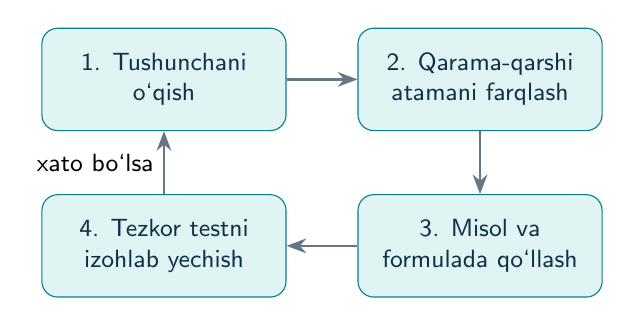
\begin{tikzpicture}[
  node distance=8mm and 9mm,
  every node/.style={font=\sffamily\small,align=center},
  box/.style={rounded corners=2mm,minimum width=31mm,minimum height=13mm,
    draw=Teal,fill=Aqua,text=Navy},
  arrow/.style={-{Stealth[length=2.5mm]},thick,draw=Muted}
]
\node[box] (read) {1. Tushunchani\\o‘qish};
\node[box,right=of read] (contrast) {2. Qarama-qarshi\\atamani farqlash};
\node[box,below=of contrast] (apply) {3. Misol va\\formulada qo‘llash};
\node[box,left=of apply] (test) {4. Tezkor testni\\izohlab yechish};
\draw[arrow] (read) -- (contrast);
\draw[arrow] (contrast) -- (apply);
\draw[arrow] (apply) -- (test);
\draw[arrow] (test) -- node[left]{xato bo‘lsa} (read);
\end{tikzpicture}
\end{center}

\section*{Uch xil o‘lchov yozuvini aralashtirmang}

\begin{tabularx}{\textwidth}{@{}L{34mm}L{35mm}Y@{}}
\toprule
\textbf{Yozuv} & \textbf{Qiymat} & \textbf{Qayerda uchraydi?}\\
\midrule
\(1~\mathrm{kB}\) & \(1000~\B\) & SI, ayrim ishlab chiqaruvchilar va tarmoq konteksti.\\
\(1~\mathrm{KiB}\) & \(1024~\B\) & IEC ikkilik prefiksi, texnik jihatdan aniq yozuv.\\
``1 KB'' \(=1024~\B\) & test shartiga ko‘ra &
Ko‘plab maktab darsliklarining an’anaviy modeli.\\
\bottomrule
\end{tabularx}

\begin{exam}
Masalada birliklar ta’rifi berilgan bo‘lsa, aynan o‘sha ta’rifni ishlating.
Berilmagan bo‘lsa, maktab testida odatda \(1~\mathrm{KB}=1024~\B\)
qabul qilinadi; real standart savolida esa kB va KiB farqlanadi.
\end{exam}


\mainmatter
\part{I QISM. AXBOROT VA RAQAMLI SAVODXONLIK ASOSLARI}
\chapter{Informatika, ma'lumot, axborot va bilim}

\begin{learningbox}
Bob yakunida siz informatikaning predmetini tushuntirasiz; informatika, AKT va raqamli texnologiyani farqlaysiz; ma'lumot--axborot--bilim zanjirini tahlil qilasiz; xabar, signal va tashuvchini ajratasiz; analog va raqamli axborot hamda axborotlashgan jamiyat mohiyatini izohlaysiz.
\end{learningbox}
\chapterintro{Axborot tushunchasini to'g'ri anglamasdan kodlash, hajm, media va qidiruv mavzularini mustahkam o'zlashtirib bo'lmaydi. Bu bob barcha keyingi boblar uchun konseptual poydevor yaratadi.}

\section{Informatika fanining predmeti, vazifalari va rivojlanishi}
\begin{definition}
\term{Informatika} -- axborotni yaratish, yig'ish, saqlash, qayta ishlash, izlash, uzatish, taqdim etish, himoyalash va bu jarayonlarni avtomatlashtirishning usul hamda vositalarini o'rganuvchi fan.
\end{definition}
Informatikaning vazifasi faqat kompyuterni ishlatishni o'rgatish emas. U axborot jarayonlarini modellashtirish, algoritmlash, texnik va dasturiy vositalarni tanlash, natijani baholash, xavfsizlik hamda raqamli madaniyatni ham qamrab oladi. Fan hisoblash texnikasi, kibernetika, aloqa, mantiq va dasturlash rivoji bilan shakllangan; zamonaviy bosqichda ma'lumotlar, sun'iy intellekt va raqamli xizmatlar uning qo'llanish maydonini kengaytirdi.

\section{Informatika, AKT va raqamli texnologiya}
\begin{tabularx}{\textwidth}{>{\bfseries\color{bookblue}}p{34mm}X}
\toprule
Tushuncha & Asosiy mazmun\\
\midrule
Informatika & Axborot jarayonlarining nazariyasi, usullari va avtomatlashtirilishi haqidagi fan.\\
AKT & Axborotni qayta ishlash va masofaga uzatishda kompyuter hamda kommunikatsiya vositalaridan birgalikda foydalanish sohasi.\\
Raqamli texnologiya & Axborotni diskret kodlarda ifodalab, elektron qurilma va dastur bilan qayta ishlaydigan texnologiya.\\
\bottomrule
\end{tabularx}
\begin{clarify}
AKT kommunikatsiya tarkibini alohida urg'ulaydi; raqamli texnologiya esa axborotning kodlangan shakliga va raqamli jarayonga urg'u beradi. Uch atama yaqin, lekin aynan bir xil emas.
\end{clarify}

\section{Ma'lumotdan bilimga va axborot modeli}
\subsection{Ma'lumotdan bilimga}
\begin{definition}
\term{Ma'lumot} \eng{data} -- hali talqin qilinmagan yoki muayyan vaziyatga bog'lanmagan raqam, harf, ramz, tovush, tasvir yoki kuzatuv.
\end{definition}
\begin{definition}
\term{Axborot} \eng{information} -- kontekst va mazmun berilib, qabul qiluvchi uchun ma'no kasb etgan ma'lumot.
\end{definition}
\begin{definition}
\term{Bilim} \eng{knowledge} -- axborotning tajriba, qoida va avvalgi tushunchalar bilan bog'lanib, xulosa chiqarish yoki harakat qilishga xizmat qiladigan o'zlashtirilgan shakli.
\end{definition}

\begin{center}
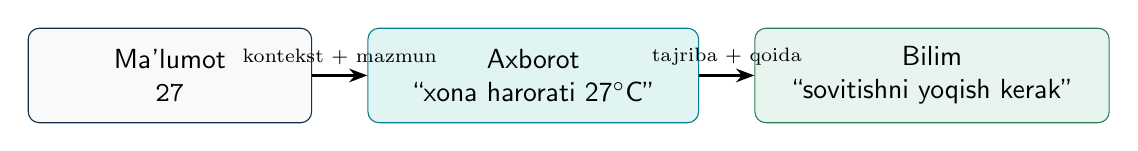
\begin{tikzpicture}[node distance=7mm, every node/.style={font=\sffamily,align=center}]
\node[draw=navy,fill=paper,rounded corners,minimum width=36mm,minimum height=12mm] (d) {Ma'lumot\\\texttt{27}};
\node[draw=teal,fill=paleteal,rounded corners,minimum width=42mm,minimum height=12mm,right=of d] (i) {Axborot\\``xona harorati 27$^\circ$C''};
\node[draw=greenx,fill=palegreen,rounded corners,minimum width=45mm,minimum height=12mm,right=of i] (k) {Bilim\\``sovitishni yoqish kerak''};
\draw[-{Stealth},thick] (d)--node[above,font=\scriptsize]{kontekst + mazmun}(i);
\draw[-{Stealth},thick] (i)--node[above,font=\scriptsize]{tajriba + qoida}(k);
\end{tikzpicture}
\end{center}

\begin{attest}
Bir xil belgi turli kontekstda boshqa axborot beradi. ``42'' kontekstsiz ma'lumot; ``50 savoldan 42 tasi to'g'ri'' esa axborot. ``Bu natija o'tish chegarasidan yuqori'' -- bilimga tayangan xulosa.
\end{attest}

\subsubsection{Bilimlar bazasining ikki ma'nosi}
\begin{enumerate}
\item \textbf{Inson nuqtayi nazaridan:} o'rganish va tajriba orqali shakllangan fakt, qoida va tushunchalar majmui.
\item \textbf{Axborot tizimida:} ekspert tizimi xulosa chiqarishi uchun saqlangan faktlar va ``agar -- u holda'' qoidalari.
\end{enumerate}
Oddiy ma'lumotlar bazasi yozuvlarni tartibli saqlaydi; bilimlar bazasi faktlar o'rtasidagi mantiqiy munosabatni ham ifodalashi mumkin.

\subsection{Axborotning mohiyatiga yondashuvlar}
\begin{tabularx}{\textwidth}{>{\bfseries\color{teal}}p{36mm}X}
\toprule
Yondashuv & Mazmun\\
\midrule
Hissiy-idrokiy & Borliqdagi narsa va hodisalarning sezgi a'zolari orqali ongda aks etishi.\\
Mazmuniy & Xabar qabul qilinganda hosil bo'lgan ma'no.\\
Kibernetik & Boshqaruv tizimining muhitga moslashishi va qaror qabul qilishi uchun foydalaniladigan mazmun.\\
Shennoncha & Natija haqidagi noaniqlikning kamayishi; axborot miqdori ehtimollik bilan bog'lanadi.\\
\bottomrule
\end{tabularx}

\begin{clarify}
Shennon nazariyasida axborot miqdori xabarning haqiqat yoki foydali ekanini o'lchamaydi. Noto'g'ri xabar ham bitlarda hajmga ega, lekin sifat jihatidan ishonchsiz bo'lishi mumkin.
\end{clarify}

\subsection{Obyekt, axborot obyekti, xabar, signal va tashuvchi}
\begin{description}[style=nextline,leftmargin=0mm]
\item[\term{Obyekt}] O'rganilayotgan narsa, hodisa, jarayon yoki shaxs.
\item[\term{Axborot obyekti}] Axborotni ifodalovchi matn, rasm, jadval, audioyozuv, video, model yoki hujjat.
\item[\term{Xabar}] Axborotni jo'natuvchidan qabul qiluvchiga yetkazish uchun tuzilgan belgilar yoki signallar ketma-ketligi.
\item[\term{Signal}] Axborotni kanal bo'ylab tashuvchi fizik holat yoki jarayon: kuchlanish, yorug'lik impulsi, radioto'lqin, tovush to'lqini.
\item[\term{Axborot tashuvchi}] Axborot qayd etiladigan moddiy muhit: qog'oz, disk, SSD, flesh-xotira, magnit tasma, optik disk.
\end{description}

\begin{warningbox}
Axborot va tashuvchi bir narsa emas. Bir matn qog'ozda, SSDda yoki bulutda saqlanishi mumkin; tashuvchi o'zgarsa ham mazmun o'zgarmasligi mumkin.
\end{warningbox}

\subsection{Inson va kompyuter axborotni qanday qabul qiladi?}
Inson axborotni ko'rish, eshitish, hid, ta'm va teri sezgisi orqali oladi. Kompyuter esa sensor yoki kiritish qurilmasi bilan fizik kattalikni o'lchaydi, analog signalni raqamli qiymatga aylantiradi va kod sifatida qayta ishlaydi. Kamera yorug'likni, mikrofon tovushni, termodatchik haroratni, klaviatura esa tugma holatini kodlaydi.


\section{Obyekt va hodisa}
\term{Obyekt} -- o'rganilayotgan narsa, shaxs, jarayon yoki tizim. \term{Hodisa} -- ma'lum vaqt va sharoitda sodir bo'ladigan voqea yoki o'zgarish. Obyekt haqidagi xossa ma'lumot bo'lishi mumkin; hodisa esa shu obyekt holatining o'zgarishini qayd etadi. Masalan, ``sensor'' obyekt, ``haroratning 30 darajaga ko'tarilishi'' hodisadir.

\section{Analog va raqamli axborot}
\begin{definition}
\term{Analog axborot} -- uzluksiz o'zgaradigan fizik signal xususiyatlari bilan ifodalangan axborot. \term{Raqamli axborot} -- alohida kod qiymatlari ketma-ketligi bilan ifodalangan axborot.
\end{definition}
Tabiiy nutq havoda uzluksiz tovush to'lqinidir. Mikrofon va ADC uni vaqt bo'yicha namunalab, sonli kodlarga aylantiradi. Raqamlashtirish nusxalash, qayta ishlash va uzatishni yengillashtiradi, biroq namunalash va kvantlash sabab ideal analog signalning barcha nozikligi saqlanmasligi mumkin.

\section{Axborotlashgan jamiyat}
\begin{definition}
\term{Axborotlashgan jamiyat} -- iqtisod, boshqaruv, ta'lim va kundalik hayotda axborotni yaratish, qayta ishlash va tarqatish asosiy resurs hamda faoliyatga aylangan jamiyat.
\end{definition}
Bunday jamiyatda raqamli xizmatlar ish tezligini oshiradi, masofani qisqartiradi va yangi kasblarni yaratadi. Shu bilan birga raqamli tengsizlik, maxfiylik, noto'g'ri axborot va kompetensiya muammolari kuchayishi mumkin. Demak, texnologik imkoniyat bilan raqamli mas'uliyat birga rivojlanishi kerak.
\section{Chuqurlashtirish: fan, tizim va aloqa modeli}
\subsection{Fanlar va atamalar orasidagi tarixiy bog'lanish}
\term{Informatika} atamasi ko'plab darsliklarda fransuzcha \eng{information automatique} - “axborotni avtomatik qayta ishlash” birikmasi bilan izohlanadi. Ingliz tilidagi \eng{Computer Science} esa hisoblash, algoritm va kompyuter tizimlarini chuqurroq nazariy o'rganishga urg'u beradi. Amaliy hayotda informatika, axborot texnologiyalari va AKT o'zaro kesishadi, lekin aynan bir tushuncha emas.

\begin{tabularx}{\textwidth}{>{\sffamily\bfseries}p{0.22\textwidth}X}
\toprule
Yo'nalish & Markaziy savol\\
\midrule
Informatika & Axborotni qanday ifodalash, qayta ishlash va boshqarish mumkin?\\
Axborot texnologiyalari & Axborot bilan ishlash uchun qaysi qurilma, dastur va usullar qo'llanadi?\\
AKT / ICT & Axborotni qayta ishlash bilan birga uni aloqa vositalari orqali qanday almashish mumkin?\\
Computer Science & Hisoblashning nazariy modeli, algoritm, dastur va kompyuter tizimlari qanday ishlaydi?\\
Kibernetika & Tizimlarda axborot, boshqaruv va qayta aloqa qanday tashkil etiladi?\\
Hujjatshunoslik / dokumentalistika & Axborotni hujjatlarda qayd etish, saqlash, qidirish va uzatish qanday tashkil qilinadi?\\
\bottomrule
\end{tabularx}

\subsubsection{Axborot tushunchasiga turli qarashlar}
Axborotga yagona, barcha sohalar uchun bir xil ta'rif berish qiyin. Darslik va ma'ruzada uch yondashuv uchraydi:
\begin{itemize}
\item \textbf{Bilish yondashuvi:} axborot insonning borliqni bilishiga xizmat qiladi; bilim esa bog'langan va qo'llaniladigan axborotdir.
\item \textbf{Noaniqlik yondashuvi:} xabar qabul qilinganda noaniqlik kamayadi. Klod Shennonning axborot nazariyasi aynan miqdoriy noaniqlikka e'tibor beradi.
\item \textbf{Boshqaruv yondashuvi:} Norbert Viner axborotni tirik organizm va texnik tizimning tashqi muhitga moslashuvi, boshqaruvi va qayta aloqasi bilan bog'laydi.
\end{itemize}
Bu qarashlar bir-birini inkor etmaydi: biri ma'no va bilimni, biri miqdorni, biri tizimdagi vazifani yoritadi.

\begin{casebox}{Bitta hodisaga uch nuqtayi nazar}
Sinf harorati 30°C bo'ldi. O'lchov qiymati - ma'lumot; “xona me'yordan issiq” degan talqin - axborot; derazani ochish yoki konditsionerni yoqish qarori - bilim va boshqaruv harakati. Agar keyingi o'lchov natijasiga qarab qurilma o'z ishini o'zgartirsa, qayta aloqa yuzaga keladi.
\end{casebox}
\subsection{Axborot almashishning to'liq modeli}
Axborot faqat manbadan qabul qiluvchiga “ko'chmaydi”. U avval xabar shakliga keltiriladi, kodlanadi, signal orqali kanal bo'ylab uzatiladi, qabul qiluvchi tomonidan qayta tiklanadi va talqin qilinadi.

\begin{center}
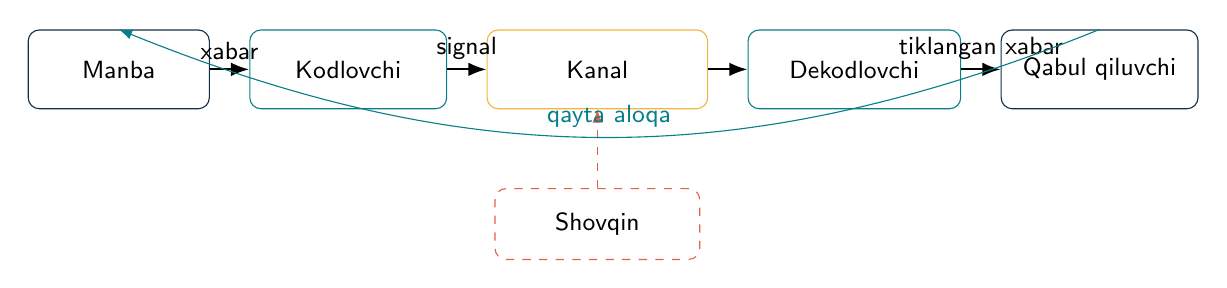
\begin{tikzpicture}[node distance=8mm and 5mm,every node/.style={font=\sffamily\small,align=center}]
\node[draw=Deep,rounded corners,minimum width=23mm,minimum height=10mm] (s) {Manba};
\node[draw=Blue,rounded corners,minimum width=25mm,minimum height=10mm,right=of s] (e) {Kodlovchi};
\node[draw=Gold,rounded corners,minimum width=28mm,minimum height=10mm,right=of e] (c) {Kanal};
\node[draw=Blue,rounded corners,minimum width=27mm,minimum height=10mm,right=of c] (d) {Dekodlovchi};
\node[draw=Deep,rounded corners,minimum width=25mm,minimum height=10mm,right=of d] (r) {Qabul qiluvchi};
\node[below=10mm of c,draw=Brick,dashed,rounded corners,minimum width=26mm,minimum height=9mm] (n) {Shovqin};
\draw[-{Latex},thick] (s)--node[above]{xabar}(e);
\draw[-{Latex},thick] (e)--node[above]{signal}(c);
\draw[-{Latex},thick] (c)--(d);
\draw[-{Latex},thick] (d)--node[above]{tiklangan xabar}(r);
\draw[-{Latex},Brick,dashed] (n)--(c);
\draw[-{Latex},Teal,bend left=22] (r.north) to node[above]{qayta aloqa} (s.north);
\end{tikzpicture}
\end{center}

\begin{definitionbox}{Model elementlari}
\begin{itemize}
\item \term{Xabar} - uzatiladigan mazmunning ifodasi: gap, raqam, rasm, tovush yoki buyruq.
\item \term{Kodlovchi} - xabarni uzatishga mos kod yoki signalga aylantiradi.
\item \term{Kanal} - signal o'tadigan fizik yoki mantiqiy yo'l: havo, kabel, optik tola, radioaloqa.
\item \term{Shovqin} - signalni buzuvchi yoki xabarni noto'g'ri qabul qilishga olib keluvchi ta'sir.
\item \term{Dekodlovchi} - signaldan xabarni qayta tiklaydi.
\item \term{Qayta aloqa} - qabul qiluvchi natijasi manbaga qaytib, keyingi harakatni o'zgartiradi.
\end{itemize}
\end{definitionbox}

\subsubsection{Tashuvchi va kanalni aralashtirmang}
\term{Tashuvchi} axborotni vaqt davomida saqlaydi: qog'oz, xotira kartasi, qattiq disk, inson xotirasi. \term{Kanal} esa signalni makonda uzatadi. Bitta obyekt turli vaziyatda turli rol o'ynashi mumkin. Masalan, optik disk saqlash tashuvchisi; undan ma'lumot o'qilayotganda lazer nuri signal vazifasini bajaradi.
\section{Bob bo'yicha mustahkamlash savollari}
\begin{enumerate}
\item Informatika, AKT va raqamli texnologiyaning umumiy va farqli tomonlarini yozing.
\item Ma'lumot, axborot va bilim zanjirida kontekst hamda tajribaning rolini tushuntiring.
\item Xabar, signal va tashuvchini bir aloqa misolida ajrating.
\item Kompyuter axborotni inson kabi ``sezadimi''? Javobni kiritish qurilmasi va kodlash bilan asoslang.
\item Axborotlashgan jamiyatning ikki imkoniyati va ikki xavfini yozing.
\end{enumerate}

\chapter{Axborotning turlari, shakllari, xossalari va manbalari}

\begin{learningbox}
Bob yakunida bir axborotni turli mezonlar bo'yicha tasniflaysiz; statik/dinamik va uzluksiz/diskret tushunchalarni farqlaysiz; ochiq, ommaviy, shaxsiy va maxfiy axborotni ajratasiz; manba turlarini uch mustaqil mezonda tahlil qilasiz; sifat xossalarining qarorga ta'sirini baholaysiz.
\end{learningbox}
\chapterintro{Axborotga bitta yorliq yetmaydi. Bir obyekt shakli, qabul kanali, yangilanishi, kirish darajasi, manbasi va sifati bo'yicha bir vaqtning o'zida turlicha tasniflanadi.}

\section{Kirish darajasiga ko'ra axborot}
\begin{longtable}{>{\bfseries\color{bookblue}}p{30mm}p{55mm}p{55mm}}
\toprule
Tur & Mazmun & Misol\\
\midrule
\endfirsthead\toprule Tur & Mazmun & Misol\\\midrule\endhead
Ochiq & Qonuniy cheklovsiz foydalanish uchun e'lon qilingan & ochiq statistik to'plam\\
Ommaviy & Keng jamoatchilikka tarqatilgan, ammo mualliflik va foydalanish shartlari saqlanishi mumkin & yangilik sayti maqolasi\\
Shaxsiy & Muayyan shaxsga tegishli yoki uni aniqlashga yordam beradigan & telefon raqami, baholar\\
Maxfiy & Faqat vakolatli shaxslar ko'rishi kerak bo'lgan & parol, tibbiy yoki xizmat siri\\
\bottomrule
\end{longtable}
\begin{attest}
``Internetda ochiq turibdi'' degani ``cheklovsiz qayta ishlatish mumkin'' degani emas. Ommaviy ko'rinish mualliflik huquqi va shaxsiy ma'lumot talablarini bekor qilmaydi.
\end{attest}

\section{Manbalarni uch mustaqil mezonda ko'rish}
\begin{tabularx}{\textwidth}{>{\bfseries\color{booknavy}}p{32mm}X}
\toprule
Mezon & Juftlik va savol\\
\midrule
Hosil bo'lishi & Birlamchi / ikkilamchi: ma'lumot aynan shu vazifa uchun birinchi marta yig'ildimi?\\
Aloqa usuli & Bevosita / bilvosita: tadqiqotchi asl obyekt yoki hodisani to'g'ridan-to'g'ri kuzatdimi?\\
Tashkilot chegarasi & Ichki / tashqi: manba tashkilot ichidanmi yoki tashqaridanmi?\\
\bottomrule
\end{tabularx}
Bir manba birlamchi, bevosita va ichki bo'lishi mumkin; boshqa manba ikkilamchi, bilvosita va tashqi bo'lishi mumkin. Bu mezonlarni aralashtirmaslik kerak.

\section{Axborot turlari, shakllari va sifat xossalari}
\begin{keywordbox}
\term{matnli}, \term{sonli}, \term{grafik}, \term{audio}, \term{video}, \term{multimedia}, \term{analog}, \term{raqamli}, \term{uzluksiz}, \term{diskret}, \term{statik}, \term{dinamik}, \term{aniqlik}, \term{ishonchlilik}, \term{dolzarblik}, \term{to'liqlik}, \term{moslik}, \term{tafsilot darajasi}.
\end{keywordbox}

\subsection{Ifodalanish shakliga ko'ra}
\begin{tabularx}{\textwidth}{>{\bfseries\color{navy}}p{30mm}X p{45mm}}
\toprule
Shakl & Mazmun & Misol\\
\midrule
Matnli & Harf, raqam, tinish belgisi va boshqa belgilar ketma-ketligi & maqola, SMS, dastur kodi\\
Sonli & Miqdor va hisoblashga yo'naltirilgan qiymatlar & baho, narx, harorat\\
Grafik & Rasm, chizma, diagramma, xarita & fotosurat, sxema\\
Tovushli & Nutq, musiqa, shovqin signali & podkast, qo'ng'iroq\\
Video & Vaqt bo'yicha ketma-ket kadr va ko'pincha audio & dars videosi\\
Multimedia & Bir nechta media shaklining integratsiyasi & interaktiv taqdimot, veb-sahifa\\
\bottomrule
\end{tabularx}

\subsection{Qabul qilish kanaliga ko'ra}
Axborot \textbf{vizual}, \textbf{audial}, \textbf{taktil}, \textbf{hid} va \textbf{ta'm} orqali qabul qilinishi mumkin. Raqamli tizimlar uchun bu kanallar sensorlar bilan ifodalanadi. Bir xabar bir necha kanalga ega bo'lishi mumkin: subtitrli video vizual va audial axborotni birlashtiradi.

\subsection{Analog va raqamli; uzluksiz va diskret}
\begin{definition}
\term{Analog axborot} -- qiymati vaqt yoki makonda uzluksiz o'zgaradigan signal bilan ifodalangan axborot.
\end{definition}
\begin{definition}
\term{Raqamli axborot} -- qiymati alohida sonlar yoki kodlar ketma-ketligi bilan ifodalangan axborot.
\end{definition}
\begin{definition}
\term{Diskret axborot} -- ajratilgan holat yoki belgilar orqali ifodalanadigan axborot; \term{uzluksiz axborot} esa oraliq qiymatlarning cheksiz ko'pini qabul qilishi mumkin.
\end{definition}

Analog va uzluksiz ko'pincha birga, raqamli va diskret ham ko'pincha birga uchraydi, ammo mezonlar aynan bir xil emas. Masalan, raqamli audio diskret namunalardan iborat; uning manbai bo'lgan tabiiy tovush uzluksiz signal.

\subsection{Statik va dinamik axborot}
\begin{definition}
\term{Statik ma'lumot} -- odatda o'zgarmaydigan yoki faqat qo'lda tahrir qilinganda yangilanadigan ma'lumot.
\end{definition}
\begin{definition}
\term{Dinamik ma'lumot} -- manba yoki ma'lumotlar bazasi o'zgarganda foydalanuvchi sahifani qo'lda tahrir qilmasdan avtomatik yangilanadigan ma'lumot.
\end{definition}

\begin{attest}
``Veb-saytdagi ma'lumot o'zgarishi mumkin'' degani uning dinamik ekanini isbotlamaydi. Statik sahifa ham muallif tahriri bilan o'zgaradi. Dinamik ma'lumotning farqi -- asosiy manba o'zgarganda avtomatik yangilanishi.
\end{attest}

\subsection{Axborot sifatining mezonlari}
\begin{longtable}{>{\bfseries\color{teal}}p{31mm}p{56mm}p{66mm}}
\toprule
Mezon & Savol & Izoh\\
\midrule
\endfirsthead
\toprule Mezon & Savol & Izoh\\\midrule\endhead
Aniqlik / to'g'rilik & Qiymat xatosizmi? & 18 yosh o'rniga 81 yozilsa, axborot noto'g'ri.\\
Ishonchlilik & Manbaga ishonish mumkinmi? & Muallif, dalil, tekshirish usuli va manfaatlar baholanadi.\\
Dolzarblik / moslik & Maqsadga aloqadormi? & Avtobus jadvali poyezd safarini rejalash uchun dolzarb emas.\\
Muddati / yangiligi & Hali amaldami? & Eski narx yoki eskirgan qonun xato qarorga olib keladi.\\
To'liqlik & Zarur qismlar bormi? & Manzil ko'cha nomi bilan, ammo uy raqamisiz berilsa, yetarli emas.\\
Tafsilot darajasi & Yetarli, ammo ortiqcha emasmi? & Juda kam tafsilot ishni bajartirmaydi; juda ko'p tafsilot asosiy fikrni yashiradi.\\
Obyektivlik & Fakt va xulosa ajratilganmi? & Reklama manbasi mahsulot kamchiligini yashirishi mumkin.\\
Tushunarlilik & Auditoriya talqin qila oladimi? & Mutaxassis termini boshlang'ich o'quvchi uchun izoh talab qiladi.\\
Foydalilik & Qaror yoki vazifaga yordam beradimi? & To'g'ri axborot ham vazifaga aloqasiz bo'lsa foydasiz.\\
Qulaylik / mavjudlik & Kerakli odam o'z vaqtida ola oladimi? & Maxfiylik bilan mavjudlik muvozanat talab qiladi.\\
\bottomrule
\end{longtable}

\begin{warningbox}
Xossalar bir-birini kafolatlamaydi. Ishonchli manba eski axborot berishi, to'liq hisobot dolzarb bo'lmasligi, aniq raqam esa noto'g'ri obyektga tegishli bo'lishi mumkin.
\end{warningbox}

\begin{examplebox}
Maktab imtihon jadvali uchun sifat tekshiruvi: fan nomlari va vaqtlar to'g'ri bo'lishi -- aniqlik; joriy yilniki bo'lishi -- muddati; barcha sinflar kiritilishi -- to'liqlik; o'quvchiga kerakli ustunlar bo'lishi -- dolzarblik; rasmiy ma'muriyatdan olinishi -- ishonchlilik.
\end{examplebox}

\begin{attest}Tasvir, matn, analog/raqamli, statik/dinamik va sifat xossalari - turli tasnif mezonlari.\end{attest}

\begin{summarybox}
Axborot turi mezonga bog'liq. Sifatni bitta ``to'g'ri/noto'g'ri'' belgisi bilan emas, aniqlik, ishonchlilik, dolzarblik, muddat, to'liqlik va tafsilot darajasi kabi mustaqil mezonlar bilan baholang.
\end{summarybox}
\begin{sourcebox}
CAM1011, PDF 13--17; ICT5, PDF 13--17; ICT11, PDF 296--305; OLD, 2-bob.
\end{sourcebox}

\section{Axborot manbalari va ma'lumot yig'ish}
\begin{keywordbox}
\term{manba}, \term{birlamchi manba}, \term{ikkilamchi manba}, \term{bevosita manba}, \term{bilvosita manba}, \term{so'rovnoma}, \term{intervyu}, \term{kuzatuv}, \term{sensor}, \term{tranzaksiya ma'lumoti}, \term{tanlanma}.
\end{keywordbox}

\subsection{Manba -- kanal -- qabul qiluvchi modeli}
\begin{center}
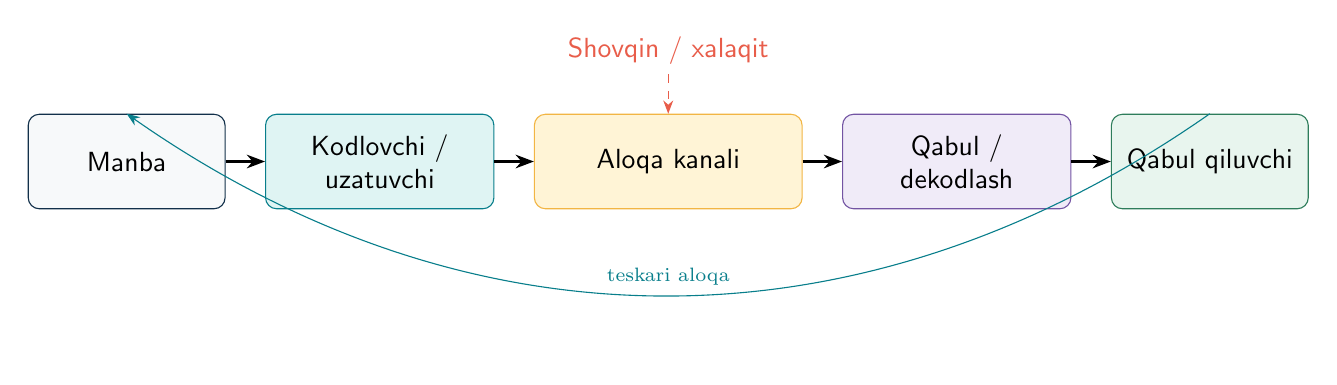
\begin{tikzpicture}[node distance=5mm, every node/.style={font=\sffamily,align=center}]
\node[draw=navy,fill=paper,rounded corners,minimum width=25mm,minimum height=12mm] (s) {Manba};
\node[draw=teal,fill=paleteal,rounded corners,minimum width=29mm,minimum height=12mm,right=of s] (e) {Kodlovchi /\\uzatuvchi};
\node[draw=gold,fill=palegold,rounded corners,minimum width=34mm,minimum height=12mm,right=of e] (c) {Aloqa kanali};
\node[draw=purple,fill=palepurple,rounded corners,minimum width=29mm,minimum height=12mm,right=of c] (d) {Qabul /\\dekodlash};
\node[draw=greenx,fill=palegreen,rounded corners,minimum width=25mm,minimum height=12mm,right=of d] (r) {Qabul qiluvchi};
\draw[-{Stealth},thick] (s)--(e);\draw[-{Stealth},thick] (e)--(c);\draw[-{Stealth},thick] (c)--(d);\draw[-{Stealth},thick] (d)--(r);
\node[above=5mm of c,text=redx] (n) {Shovqin / xalaqit};
\draw[-{Stealth},dashed,redx] (n)--(c);
\draw[-{Stealth},teal,bend left=35] (r.north) to node[above,font=\scriptsize]{teskari aloqa} (s.north);
\end{tikzpicture}
\end{center}

\subsection{Birlamchi va ikkilamchi; bevosita va bilvosita}
\begin{definition}
\term{Birlamchi yoki bevosita manba} -- aynan joriy maqsad uchun birinchi qo'ldan yig'ilgan ma'lumot.
\end{definition}
\begin{definition}
\term{Ikkilamchi yoki bilvosita manba} -- avval boshqa maqsadda yig'ilgan, keyin joriy vazifa uchun qayta ishlatiladigan ma'lumot.
\end{definition}

Darsliklarda ``bevosita/bilvosita'' va ``birlamchi/ikkilamchi'' ko'pincha bir-biriga mos ma'noda ishlatiladi. Biroq ilmiy adabiyotlarda atamalar kontekstga qarab nozik farqlanishi mumkin; testda darslik ta'rifi ustuvor.

\begin{tabularx}{\textwidth}{>{\bfseries\color{navy}}p{35mm}X X}
\toprule
 & Birlamchi / bevosita & Ikkilamchi / bilvosita\\
\midrule
Maqsad & Joriy tadqiqot uchun yig'iladi & Avvalgi maqsad uchun mavjud\\
Moslik & Odatda yuqori & Qisman mos bo'lishi mumkin\\
Narx va vaqt & Ko'proq & Odatda kamroq\\
Nazorat & Savol va tanlanma ustidan nazorat bor & Yig'ish usuli ustidan nazorat yo'q\\
Yangiligi & Joriy bo'lishi mumkin & Eskirgan bo'lishi mumkin\\
Misol & o'quvchilardan yangi so'rov & o'tgan yilgi hisobot\\
\bottomrule
\end{tabularx}

\subsection{Ma'lumot yig'ish usullari}
\begin{longtable}{>{\bfseries\color{teal}}p{31mm}p{53mm}p{65mm}}
\toprule
Usul & Kuchli tomoni & Cheklovi\\
\midrule
\endfirsthead\toprule Usul & Kuchli tomoni & Cheklovi\\\midrule\endhead
So'rovnoma & Ko'p odamdan standart javob; avtomatik tahlil oson & Savol tarafkash bo'lishi, javob yuzaki yoki yolg'on bo'lishi mumkin\\
Intervyu & Chuqur izoh va aniqlashtiruvchi savol & Vaqt va xarajat ko'p; intervyuer ta'siri\\
Kuzatuv & Haqiqiy xatti-harakatni ko'rish & Kuzatilayotgan odam xulqini o'zgartirishi; talqin subyektiv\\
O'lchov/sensor & Tez, takroriy va avtomatik; katta hajm & Kalibrlash xatosi, nosozlik, maxfiylik\\
Tajriba & Sabab-oqibatni nazoratli tekshirish & Sun'iy sharoit real hayotni to'liq aks ettirmasligi\\
Tranzaksiya yozuvi & Real faoliyatdan avtomatik hosil bo'ladi & Dastlab boshqa maqsad uchun yig'ilgan; kontekst yetishmasligi\\
Hujjat/tadqiqot & Tez va arzon ikkilamchi manba & Eskirish, tarafkashlik va aniqlik muammosi\\
\bottomrule
\end{longtable}

\subsubsection{Tanlanma va tarafkashlik}
Butun populyatsiyani o'rganish qimmat bo'lsa, \term{tanlanma} olinadi. Tanlanma yetarli kattalikda va vakillik xususiyatiga ega bo'lishi kerak. Faqat eng faol foydalanuvchilarni so'rash \term{tanlanma tarafkashligi}ni keltirib chiqaradi. Savolning ``Siz ham foydali yangi tizimni qo'llab-quvvatlaysizmi?'' kabi yo'naltiruvchi shakli esa \term{savol tarafkashligi}ni yuzaga keltiradi.

\subsection{Statik va dinamik manba}
Statik manbada ma'lumot faqat fayl yoki sahifa tahrir qilinganda o'zgaradi. Dinamik manba ma'lumotlar bazasi, sensor, jonli xizmat yoki hisoblash natijasi bilan bog'langan bo'lib, asosiy manba yangilansa avtomatik o'zgaradi.

\begin{attest}
Biror saytning ``tez-tez yangilanishi'' dinamiklikning o'zi emas. Yangilanish qo'lda kiritiladimi yoki asosiy ma'lumot manbasidan avtomatik keladimi -- shuni tekshiring.
\end{attest}

\begin{attest}Manba turidan tashqari tanlama, maqsad, sana va yig'ish usuli ham baholanadi.\end{attest}

\begin{summarybox}
Manbani baholashda maqsad, yig'ish usuli, vaqt, tanlanma, xarajat va xolislikni birgalikda tekshiring. Birlamchi manba har doim mukammal emas; noto'g'ri savol yoki nosoz sensor birlamchi ma'lumotni ham sifatsiz qiladi.
\end{summarybox}
\begin{sourcebox}
CAM1011, PDF 13--16; CAM9, axborot yig'ish va tizim hayot sikli bo'limlari; ICT11, ma'lumotlar bazasi va Big Data bo'limlari; OLD, 3-bob.
\end{sourcebox}
\section{Chuqurlashtirilgan tasnif, sifat va taqdim etish}
\subsection{Axborotni qo'shimcha tasniflash mezonlari}
Darsliklarda bir xil obyekt turli mezonlar bo'yicha tasniflanadi. To'g'ri javob mezonni aniq aytishi kerak.

\subsubsection{Miqdoriy va sifat ma'lumoti}
\term{Miqdoriy ma'lumot} son bilan o'lchanadi yoki sanaladi: harorat, o'quvchilar soni, fayl hajmi. \term{Sifat ma'lumoti} toifa yoki xususiyatni bildiradi: rang, qurilma turi, fikr, holat. “5 ta ko'k fayl” yozuvida 5 - miqdoriy, ko'k - sifat ma'lumoti.

\subsubsection{Strukturali, yarim strukturali va strukturasiz ma'lumot}
\begin{tabularx}{\textwidth}{>{\sffamily\bfseries}p{0.22\textwidth}X}
\toprule
Turi & Belgisi va misol\\
\midrule
Strukturali & Oldindan belgilangan maydon va tartibga ega: elektron jadval, ma'lumotlar bazasi yozuvi.\\
Yarim strukturali & Umumiy belgilash yoki teglar bor, lekin qat'iy jadval emas: elektron pochta xabari, JSON/XML hujjati.\\
Strukturasiz & Qat'iy maydonlarga ajratilmagan: erkin matn, foto, audio, video.\\
\bottomrule
\end{tabularx}
Bu tasnif “matnli/grafik/audio” shakl tasnifini almashtirmaydi. Masalan, surat strukturasiz grafik ma'lumot bo'lishi mumkin.

\subsubsection{Obyektiv va subyektiv axborot}
\term{Obyektiv axborot} tekshiriladigan o'lchov yoki dalilga tayanadi. \term{Subyektiv axborot} shaxsiy qarash, his yoki bahoni ifodalaydi. Subyektiv axborot avtomatik ravishda “yolg'on” emas; u fikr sifatida to'g'ri belgilanishi kerak.
\subsection{Axborot sifati: kengaytirilgan model}
Axborot sifati bitta xossa bilan emas, bir nechta mezonning birgalikdagi holati bilan baholanadi.

\begin{longtable}{>{\sffamily\bfseries}p{0.19\textwidth}p{0.31\textwidth}p{0.40\textwidth}}
\toprule
Xossa & Savol & Muammo namunasi\\
\midrule
\endfirsthead
\toprule
Xossa & Savol & Muammo namunasi\\
\midrule
\endhead
To'g'rilik / aniqlik & Qiymat xatosiz va real holatga mosmi? & 90,30 o'rniga 903,00 yozilgan.\\
Ishonchlilik & Manba, usul va dalilga ishonish mumkinmi? & Muallifi noma'lum post, tekshirilmagan da'vo.\\
Dolzarblik / moslik & Ma'lumot aynan vazifa uchun kerakmi? & Poyezd jadvali kerak bo'lganda avtobus jadvali berildi.\\
Yangilik / muddat & Axborot foydalanish vaqtida eskirmaganmi? & Besh yil avvalgi narx asosida qaror qilish.\\
To'liqlik & Qaror uchun zarur qismlar bormi? & Manzil bor, lekin uy raqami yo'q.\\
Tafsilot darajasi & Juda kam yoki ortiqcha tafsilot bormi? & Bitta vaqt kerak bo'lsa, barcha stansiyalar jadvali berilgan.\\
Tushunarlilik & Til, belgi va format auditoriyaga mosmi? & Boshlang'ich o'quvchiga izohsiz texnik jargon.\\
Obyektivlik & Tanlash va ifodalash bir tomonlama emasmi? & Faqat foydali natijalar ko'rsatilgan reklama.\\
Foydalilik / qiymat & Axborot qaror yoki vazifaga yordam beradimi? & To'g'ri, lekin foydalanuvchi maqsadiga aloqasiz ma'lumot.\\
Mavjudlik & Vakolatli foydalanuvchi kerakli paytda foydalana oladimi? & Muhim fayl bor, ammo ochish huquqi yo'q.\\
\bottomrule
\end{longtable}

\begin{casebox}{Sifat mezonlari bir-birini kafolatlamaydi}
Rasmiy tashkilotning 2020-yildagi e'loni manba jihatidan ishonchli bo'lishi mumkin, lekin bugungi qaror uchun eskirgan. Yangi ijtimoiy tarmoq posti dolzarb bo'lishi mumkin, lekin manbasi noma'lum. Shuning uchun “rasmiy” yoki “yangi” so'zining o'zi yetarli emas.
\end{casebox}
\subsection{Ma'lumot manbaini tanlash va yig'ish usullari}
\subsubsection{Birlamchi va ikkilamchi; bevosita va bilvosita}
Bu juftliklar ko'pincha bir-biriga mos keladi, lekin mezonlari farq qiladi. \term{Birlamchi manba} hodisaga eng yaqin asl dalil yoki muallifning o'z materiali. \term{Ikkilamchi manba} birlamchi materialni sharhlaydi, qayta ishlaydi yoki umumlashtiradi. \term{Bevosita ma'lumot} aynan joriy maqsad uchun yig'iladi; \term{bilvosita ma'lumot} boshqa maqsad uchun avval yig'ilgan bo'ladi.

\subsubsection{Yig'ish usullari}
\begin{tabularx}{\textwidth}{>{\sffamily\bfseries}p{0.20\textwidth}p{0.30\textwidth}X}
\toprule
Usul & Kuchli tomoni & Cheklovi\\
\midrule
Kuzatish & Haqiqiy xatti-harakatni qayd etadi & Sabab va fikrni doim ochib bermaydi\\
Intervyu & Chuqur, aniqlashtiruvchi javob & Vaqt talab qiladi, suhbatdosh ta'siri bo'lishi mumkin\\
So'rovnoma & Ko'p kishidan bir xil formatda ma'lumot & Savol tuzilishi javobni og'dirishi mumkin\\
O'lchov/sensor & Takrorlanuvchi va avtomatik qayd & Kalibrlash xatosi, qurilma nosozligi\\
Tajriba & Sabab-oqibatni sinash imkoniyati & Sun'iy sharoit va etik cheklovlar\\
Mavjud yozuvlar & Tez va arzon, katta hajm & Maqsad boshqa bo'lgan, eskirgan yoki to'liq emas\\
\bottomrule
\end{tabularx}

\subsubsection{Tanlanma va noxolislik}
Barcha aholini tekshirish imkonsiz bo'lsa, \term{tanlanma} olinadi. Tanlanma vakil bo'lishi uchun turli guruhlarni adolatli qamrab olishi kerak. Faqat informatika to'garagidagi o'quvchilardan “maktabda dasturlash qanchalik mashhur?” deb so'rash natijani yuqori tomonga og'diradi. Savolning o'zi ham noxolis bo'lishi mumkin: “Foydali elektron darslikni qo'llab-quvvatlaysizmi?” jumlasidagi “foydali” so'zi javobga ta'sir qiladi.
\subsection{Axborotni taqdim etish shaklini tanlash}
Bitta mazmun matn, jadval, diagramma, xarita, audio yoki video ko'rinishida berilishi mumkin. Shakl tanlashda auditoriya, maqsad, aniqlik, vaqt va foydalanish sharoiti hisobga olinadi.

\begin{tabularx}{\textwidth}{>{\sffamily\bfseries}p{0.21\textwidth}X}
\toprule
Maqsad & Odatda mos shakl\\
\midrule
Aniq qiymatlarni solishtirish & jadval yoki ustunli diagramma\\
Vaqt bo'yicha o'zgarish & chiziqli diagramma\\
Joylashuv va hudud & xarita\\
Bosqichni tushuntirish & sxema, oqim diagrammasi yoki animatsiya\\
Murakkab fikrni izohlash & matn + tasvir + misol\\
Ko'rish imkoniyati cheklangan auditoriya & audio tavsif, ekran o'qiydigan tuzilma\\
Eshitish imkoniyati cheklangan auditoriya & subtitr, transkript, vizual signal\\
\bottomrule
\end{tabularx}

\sourcecite{Qo'shimcha sintez: Cambridge+ 10--11-sinf, 1-bob; ICT 5- va 8-sinf; Cambridge+ 6--9-sinfdagi source material, audience va data quality bo'limlari.}

\begin{recapbox}
\begin{itemize}
\item Tasnif mezoni aytilishi shart; bir axborot bir nechta toifaga kirishi mumkin.
\item Statik/dinamik yangilanishga, uzluksiz/diskret qiymatlar tabiatiga tegishli.
\item Axborot sifati ko‘p xossali; bitta xossa boshqasini kafolatlamaydi.
\item Birlamchi/ikkilamchi manbaning originalligini, bevosita/bilvosita esa yig‘ish usulini ko‘rsatadi.
\item Ishonchli qaror uchun manba, sana, maqsad, dalil va boshqa manbalar bilan moslik tekshiriladi.
\end{itemize}
\end{recapbox}
\section{Bob bo'yicha mustahkamlash savollari}
\begin{enumerate}
\item Bitta video faylni kamida to'rt mezon bo'yicha tasniflang.
\item Statik sahifa bilan dinamik ma'lumotni farqlovchi asosiy belgi nima?
\item Birlamchi manba nega har doim ishonchli bo'lmasligi mumkin?
\item Aniqlik, ishonchlilik, dolzarblik va to'liqlikning bir-birini kafolatlamasligini misolda ko'rsating.
\item Shaxsiy va maxfiy axborot orasidagi munosabatni tushuntiring.
\end{enumerate}

\chapter{Axborot jarayonlari, izlash va raqamli madaniyat}

\begin{learningbox}
Bob yakunida axborot hayot siklini izohlaysiz; yaratishdan yo'q qilishgacha bo'lgan jarayonlarni farqlaysiz; qidiruv strategiyasi va manba baholash protokolini amalda qo'llaysiz; auditoriya, maqsad va kontekstni hisobga olasiz; elektron pochta madaniyati, netiket va raqamli iz qoidalariga amal qilasiz.
\end{learningbox}
\chapterintro{Raqamli savodxonlik kerakli axborotni topish bilan tugamaydi. Uni maqsadga mos yig'ish, tartiblash, baholash, taqdim etish va mas'uliyat bilan yo'q qilish ham zarur.}

\section{Saralash, filtrlash va guruhlashni farqlash}
\begin{tabularx}{\textwidth}{>{\bfseries\color{bookblue}}p{30mm}X p{48mm}}
\toprule
Amal & Natija & Misol\\
\midrule
Saralash & Barcha yozuvlar tanlangan mezon bo'yicha tartiblanadi & ballni kamayish tartibida\\
Filtrlash & Faqat shartga mos yozuvlar ko'rsatiladi & balli 80 dan yuqori\\
Guruhlash & Yozuvlar umumiy belgi bo'yicha toifalarga ajratiladi & sinf yoki hudud bo'yicha\\
\bottomrule
\end{tabularx}
\begin{warningbox}
Saralash ma'lumotni o'chirmaydi; faqat tartibni o'zgartiradi. Filtrlash ham odatda yozuvni o'chirmaydi, balki vaqtincha ko'rsatmaydi.
\end{warningbox}

\section{Elektron pochta madaniyati}
Professional elektron xatda mavzu satri aniq bo'ladi, salomlashish va qisqa maqsad ko'rsatiladi, ilova nomi tushunarli yoziladi, yuborishdan oldin qabul qiluvchi va fayl tekshiriladi. \textbf{CC} nusxadan xabardor bo'lishi kerak bo'lganlar uchun, \textbf{BCC} esa qabul qiluvchilarning manzillarini bir-biridan yashirish zarur bo'lganda qo'llanadi. ``Reply all'' faqat hamma ishtirokchi javobni bilishi kerak bo'lsa ishlatiladi.

\section{Netiket}
\term{Netiket} -- internetdagi hurmatli, tushunarli va xavfsiz muloqot qoidalari. Katta harflarda to'liq yozish baqirish sifatida qabul qilinishi mumkin; shaxsiy hujum, spam, tekshirilmagan xabarni ulashish va boshqa odamning ma'lumotini ruxsatsiz tarqatish noto'g'ri. Tanqid shaxsga emas, fikr yoki dalilga qaratiladi.

\section{Raqamli iz}
\begin{definition}
\term{Raqamli iz} -- foydalanuvchining raqamli faoliyati natijasida qoladigan post, qidiruv, joylashuv, kirish jurnali, cookie, metadata va boshqa yozuvlar.
\end{definition}
Faol iz foydalanuvchi ataylab yuborgan ma'lumot; passiv iz tizim tomonidan avtomatik yig'ilgan yozuvdir. Kontent o'chirilganda ham nusxa, skrinshot yoki zaxirada qolishi mumkin. Yuborishdan oldin kelajakdagi auditoriya va oqibatni baholash raqamli madaniyatning muhim qismidir.

\section{Auditoriya, maqsad va kontekst}
Axborotni taqdim etish usuli kimga, nima uchun va qaysi sharoitda berilishiga bog'liq. O'quvchiga sodda til va misol; rahbarga asosiy natija va qaror; mutaxassisga metod, birlik va cheklovlar kerak bo'lishi mumkin. Bir xil grafik telefon ekranida va bosma hisobotda boshqa o'lcham hamda tafsilotda tayyorlanadi.

\section{Axborot jarayonlari va hayot sikli}
\subsection{Axborotli jarayonlar}
\begin{definition}
\term{Axborotli jarayon} -- axborotni yaratish, qabul qilish, yig'ish, saqlash, izlash, qayta ishlash, uzatish, taqdim etish, himoyalash yoki yo'q qilish bilan bog'liq faoliyat.
\end{definition}

\begin{center}
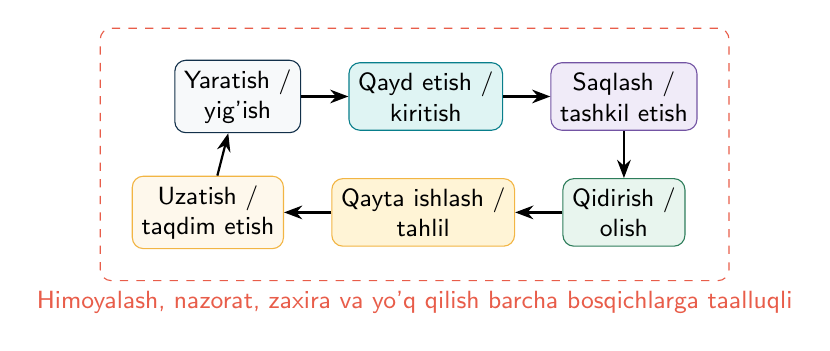
\begin{tikzpicture}[every node/.style={font=\sffamily\small,align=center},node distance=6mm]
\node[draw=navy,fill=paper,rounded corners] (a) {Yaratish /\\yig'ish};
\node[draw=teal,fill=paleteal,rounded corners,right=of a] (b) {Qayd etish /\\kiritish};
\node[draw=purple,fill=palepurple,rounded corners,right=of b] (c) {Saqlash /\\tashkil etish};
\node[draw=greenx,fill=palegreen,rounded corners,below=of c] (d) {Qidirish /\\olish};
\node[draw=gold,fill=palegold,rounded corners,left=of d] (e) {Qayta ishlash /\\tahlil};
\node[draw=orange,fill=orange!10,rounded corners,left=of e] (f) {Uzatish /\\taqdim etish};
\draw[-{Stealth},thick] (a)--(b);\draw[-{Stealth},thick] (b)--(c);\draw[-{Stealth},thick] (c)--(d);\draw[-{Stealth},thick] (d)--(e);\draw[-{Stealth},thick] (e)--(f);\draw[-{Stealth},thick] (f)--(a);
\node[draw=redx,dashed,rounded corners,fit=(a)(b)(c)(d)(e)(f),inner sep=4mm,label={[text=redx,font=\sffamily\small]below:Himoyalash, nazorat, zaxira va yo'q qilish barcha bosqichlarga taalluqli}] {};
\end{tikzpicture}
\end{center}

\subsection{Kiritish -- qayta ishlash -- chiqarish -- saqlash modeli}
\term{Kiritish} tashqi muhitdan ma'lumotni tizimga olib kiradi. \term{Qayta ishlash} hisoblash, taqqoslash, saralash, formatlash, modellashtirish yoki tasniflash orqali ma'lumotni o'zgartiradi. \term{Chiqarish} natijani foydalanuvchi yoki boshqa tizimga beradi. \term{Saqlash} esa ma'lumot va natijani keyingi foydalanish uchun saqlaydi. Teskari aloqa chiqish natijasini keyingi kirishga aylantirishi mumkin.

\begin{examplebox}
Elektron jurnal: o'qituvchi bahoni kiritadi; tizim diapazon va foydalanuvchi huquqini tekshiradi; o'rtacha bahoni hisoblaydi; natijani jadval va hisobotda chiqaradi; ma'lumotlar bazasida saqlaydi; ota-ona ko'rishi teskari aloqa va yangi harakatni yuzaga keltiradi.
\end{examplebox}

\subsection{Qayta ishlash natijasida yangi axborot}
Qayta ishlash faqat formatni almashtirish emas. U xom ma'lumotdan yangi mazmun hosil qilishi mumkin:
\begin{itemize}
\item qiymatlarni yig'ish -- umumiy natija;
\item saralash -- tartib va ustuvorlik;
\item filtrlash -- shartga mos yozuvlar;
\item taqqoslash -- farq yoki anomaliya;
\item guruhlash -- toifa va tendensiya;
\item statistik tahlil -- o'rtacha, median, korrelatsiya;
\item modellashtirish -- ehtimoliy natija yoki prognoz.
\end{itemize}

\begin{sourcebox}ICT7, PDF 4--8; ICT5, PDF 13--23; CAM1011, ma'lumot va axborot jarayonlari bo'limlari; OLD, 3--4-boblar.\end{sourcebox}
\section{Qidiruv tizimlari, kalit so'zlar va manba auditi}
\begin{keywordbox}
\term{qidiruv so'rovi}, \term{kalit so'z}, \term{indeks}, \term{saralash}, \term{filtrlash}, \term{manba}, \term{muallif}, \term{dolzarblik}, \term{ishonchlilik}, \term{fakt}, \term{fikr}, \term{dezinformatsiya}.
\end{keywordbox}

\subsection{Qidiruv tizimi qanday ishlaydi?}
\begin{enumerate}
\item \term{Crawler/spider} havolalarni kuzatib sahifalarni topadi.
\item Kontent tahlil qilinib \term{indeks}ga qo'shiladi.
\item Foydalanuvchi so'rovi token va ma'noga ajratiladi.
\item \term{Ranking} moslik, sifat, yangilik, joylashuv va boshqa signallar bo'yicha natijani tartiblaydi.
\item Natija sahifasi organik, reklama va maxsus bloklarni ko'rsatishi mumkin.
\end{enumerate}

\subsection{Samarali so'rov}
\begin{longtable}{>{\ttfamily\bfseries}p{42mm}p{54mm}p{54mm}}
\toprule
Operator/usul & Maqsad & Misol\\
\midrule
\endfirsthead\toprule Operator/usul & Maqsad & Misol\\\midrule\endhead
\texttt{"aniq ibora"} & so'z tartibini saqlash & \texttt{"axborot hajmi"}\\
\texttt{-so'z} & keraksiz ma'noni chiqarish & \texttt{python -ilon}\\
\texttt{site:domain} & bitta sayt/domen ichida & \texttt{site:edu.uz Unicode}\\
\texttt{filetype:pdf} & fayl turini cheklash & \texttt{filetype:pdf sanoq sistemasi}\\
\texttt{OR} & muqobil atama & \texttt{Vijener OR Vigenere}\\
Aniq birlik/yil & kontekstni toraytirish & \texttt{44.1 kHz 16 bit stereo formula}\\
Sinonim va tarjima & recallni oshirish & \texttt{validation data entry tekshirish}\\
\bottomrule
\end{longtable}

\subsection{Manbani baholash protokoli}
\begin{enumerate}
\item \textbf{Muallif:} kim va qaysi vakolat bilan yozgan?
\item \textbf{Maqsad:} o'rgatish, sotish, ishontirish yoki ko'ngilochar?
\item \textbf{Dalil:} manba, usul, ma'lumot va havola bormi?
\item \textbf{Sana:} mavzu uchun yetarlicha yangimi?
\item \textbf{Moslik:} savolning aynan qaysi qismini javoblaydi?
\item \textbf{Tasdiq:} mustaqil ishonchli manbalar mos keladimi?
\item \textbf{Tahrir:} xato tuzatish va nashriy nazorat bormi?
\end{enumerate}

\subsubsection{Fakt, noto'g'ri axborot va manipulyatsiya}
\term{Misinformation} -- xato bo'lsa ham ataylab aldash maqsadisiz tarqalgan ma'lumot; \term{disinformation} -- ataylab chalg'itish; \term{malinformation} -- haqiqiy ma'lumotni zarar yetkazish uchun kontekstdan uzib tarqatish. Sarlavha, rasm va statistik grafik ham manipulyatsiya qilishi mumkin.

\begin{attest}
Domenning \texttt{.org} yoki \texttt{.edu} bilan tugashi o'z-o'zidan mazmun to'g'riligini kafolatlamaydi. Muallif, dalil, sana va boshqa manbani ham tekshiring.
\end{attest}

\subsection{Tasvir, audio va video qidiruvi}
Media qidirishda format, o'lcham, litsenziya, davomiylik, manba va teskari tasvir qidiruvi muhim. Teskari qidiruv rasmning avvalgi nusxasi va kontekstini topishga yordam beradi. Media faylni yuklashdan oldin mualliflik huquqi va metadata tekshiriladi.

\subsection{Mustahkamlash: oddiydan murakkabga 3 misol}
\begin{taskbox}
\begin{enumerate}[leftmargin=7mm]
\item \textbf{Oddiy.} ``O'zbekistonda suv tejash'' mavzusiga aniqroq qidiruv so'rovi tuzing.
\item \textbf{O'rta.} Ikki sahifa topildi: biri 2018-yilgi anonim blog, ikkinchisi 2026-yilgi rasmiy tashkilot hisoboti. Qaysi birini asosiy manba qilasiz va nima uchun?
\item \textbf{Murakkab.} Ijtimoiy tarmoqdagi grafikda sonlar berilgan, lekin o'q kesilgan va manba yo'q. Uni ulashishdan oldin tekshiruv algoritmini yozing.
\end{enumerate}
\end{taskbox}

\begin{solutionbox}
\begin{enumerate}[leftmargin=7mm]
\item \textbf{Oddiy yechim.} Masalan: \texttt{"suv tejash" O'zbekiston filetype:pdf}. Aniq ibora va fayl turi natijani toraytiradi.
\item \textbf{O'rta yechim.} Asosiy manba sifatida rasmiy va yangi hisobot tanlanadi; muallif, sana, metod va dalil tekshiriladi. Blog yordamchi fikr bo'lishi mumkin, lekin anonimligi va eskirganligi zaiflik.
\item \textbf{Murakkab yechim.} 1) asl manbani topish; 2) o'q va masshtabni tekshirish; 3) raqamlarni rasmiy dataset bilan solishtirish; 4) sana va kontekstni aniqlash; 5) xulosa grafikdan ortiqcha chiqmaganini tekshirish; 6) manba bilan ulashish yoki rad etish.
\end{enumerate}
\end{solutionbox}
\begin{attest}Qidiruv tizimida yuqorida chiqish ishonchlilik kafolati emas.\end{attest}

\begin{summarybox}
Qidiruv natijasi javob emas, nomzod manbalar ro'yxati. Samarali so'rov topishni, manba auditi esa ishonishni boshqaradi.
\end{summarybox}
\begin{sourcebox}
ICT6, PDF 77--114; ICT8 SMM/CMS va platformalar; CAM5--CAM8 Internet qidiruvi; CAM9 kommunikatsiya; OLD, 15-bob.
\end{sourcebox}
\section{Axborot texnologiyasi va raqamli jamiyat}
\subsection{Axborot texnologiyasi}
\begin{definition}
\term{Axborot texnologiyasi} -- ma'lum maqsadga erishish uchun axborotni yig'ish, qayta ishlash, saqlash, uzatish va taqdim etishda qo'llanadigan usul, jarayon va vositalar majmui.
\end{definition}
Texnologiya faqat qurilma emas. Masalan, bulutli hujjat bilan hamkorlik qurilma, dastur, tarmoq, foydalanuvchi roli, versiya nazorati va xavfsizlik qoidasining birgalikdagi jarayonidir.
\subsection{Raqamli muhit va axborotlashgan jamiyat}
\term{Raqamli muhit} -- axborot raqamli shaklda yaratiladigan, saqlanadigan va almashinadigan qurilma, dastur, tarmoq va xizmatlar makoni. \term{Axborotlashgan jamiyat}da aholining katta qismi faoliyati axborotni ishlab chiqish, qayta ishlash, saqlash va tarqatish bilan bog'liq bo'ladi.

\subsubsection{Raqamli tengsizlik}
\term{Raqamli tengsizlik} -- qurilma, Internet, sifatli xizmat, ko'nikma yoki foydalanish imkoniyatidagi farq. U faqat Internet bor-yo'qligi emas; tezlik, narx, til, nogironligi bo'lgan foydalanuvchilar uchun moslik va raqamli ko'nikma ham ta'sir qiladi.
\section{Axborotning to‘liq hayotiy sikli va dalil auditi}
\subsection{Axborot hayotiy sikli va qayta ishlash amallari}
Axborot bilan ishlash bir martalik amal emas. U yaratiladi yoki yig'iladi, sifat nazoratidan o'tadi, qayta ishlanadi, saqlanadi, foydalaniladi, ulashiladi, yangilanadi, arxivlanadi va zarur bo'lmaganda xavfsiz yo'q qilinadi. Har bir bosqichda mas'uliyat va sifat talabi o'zgaradi.

\begin{center}
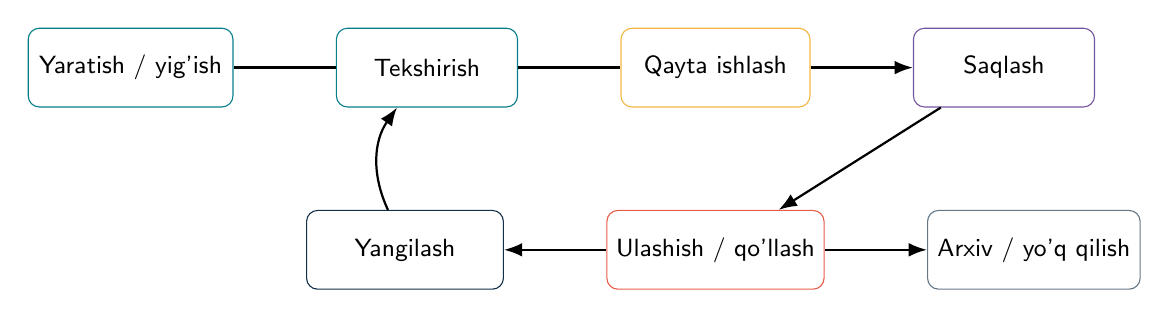
\begin{tikzpicture}[node distance=13mm,every node/.style={font=\sffamily\small,align=center}]
\node[draw=Blue,rounded corners,minimum width=26mm,minimum height=10mm] (a) {Yaratish / yig'ish};
\node[draw=Teal,rounded corners,minimum width=23mm,minimum height=10mm,right=of a] (b) {Tekshirish};
\node[draw=Gold,rounded corners,minimum width=24mm,minimum height=10mm,right=of b] (c) {Qayta ishlash};
\node[draw=Plum,rounded corners,minimum width=23mm,minimum height=10mm,right=of c] (d) {Saqlash};
\node[draw=Brick,rounded corners,minimum width=24mm,minimum height=10mm,below=of c] (e) {Ulashish / qo'llash};
\node[draw=Deep,rounded corners,minimum width=25mm,minimum height=10mm,left=of e] (f) {Yangilash};
\node[draw=Muted,rounded corners,minimum width=27mm,minimum height=10mm,right=of e] (g) {Arxiv / yo'q qilish};
\draw[-{Latex},thick] (a)--(b)--(c)--(d);
\draw[-{Latex},thick] (d)--(e);
\draw[-{Latex},thick] (e)--(f);
\draw[-{Latex},thick] (f) to[bend left=30] (b);
\draw[-{Latex},thick] (e)--(g);
\end{tikzpicture}
\end{center}

\subsubsection{Saralash, filtrlash, guruhlash va umumlashtirish}
\begin{itemize}
\item \term{Saralash} yozuvlarni tanlangan mezon bo'yicha tartiblaydi: ism bo'yicha A-Z, ball bo'yicha katta-kichik.
\item \term{Filtrlash} shartga mos yozuvlarni ko'rsatadi: balli 70 dan yuqori o'quvchilar.
\item \term{Guruhlash} o'xshash yozuvlarni toifalarga ajratadi: sinf, hudud yoki qurilma turi bo'yicha.
\item \term{Umumlashtirish} katta hajmdan ko'rsatkich chiqaradi: jami, o'rtacha, minimum, maksimum, ulush.
\item \term{Xulosa chiqarish} natijani vaziyat va dalil bilan talqin qiladi. Hisoblangan o'rtacha qiymatning o'zi hali to'liq xulosa emas.
\end{itemize}

\begin{examplebox}{Ishlangan usul. Ma'lumotni saralashdan xulosagacha \difficulty{Bosqichli tahlil}}
O'quvchilarning test ballari va sinflari berilgan. “Qaysi sinfga qo'shimcha mashg'ulot ko'proq kerak?” savoliga javob berish kerak.
\begin{solutionbox}
\begin{enumerate}
\item Noto'g'ri yoki bo'sh qiymatlarni tekshiring.
\item Yozuvlarni sinf bo'yicha guruhlang.
\item Har sinf uchun o'rtacha, median va past natijalar ulushini hisoblang.
\item Faqat o'rtachaga tayanmang: bir nechta juda yuqori ball o'rtachani oshirishi mumkin.
\item Sinflar topshiriq sharoiti bir xil bo'lganini tekshiring.
\item Dalilga mos ehtiyotkor xulosa yozing: “8-B sinfda 50 balldan past natijalar ulushi yuqori; aynan shu ko'nikmalar bo'yicha qo'shimcha mashg'ulot rejalashtirish maqsadga muvofiq.”
\end{enumerate}
\end{solutionbox}
\end{examplebox}
\subsection{Qidiruvni rejalashtirish algoritmi}
Samarali qidiruv kalit so'z yozishdan oldin boshlanadi.
\begin{enumerate}
\item \textbf{Axborot ehtiyojini aniqlang:} nima kerak, qaysi davr, qaysi hudud, qaysi daraja?
\item \textbf{Asosiy tushunchalarni ajrating:} sinonim, qisqartma va boshqa tildagi variantlarini yozing.
\item \textbf{So'rovni toraytiring:} aniq ibora, minus, \code{site:}, \code{filetype:}, sana va til filtrlari.
\item \textbf{Natijani tez tekshiring:} domen, sarlavha, sana, muallif, qisqa matn.
\item \textbf{Manbani ochib baholang:} maqsad, dalil, havola, yangilanish, tarafkashlik.
\item \textbf{Kamida ikki mustaqil manba bilan solishtiring.}
\item \textbf{Kerakli qismini qayd etib, manbasini yozib boring.}
\end{enumerate}

\subsubsection{Qo'shimcha qidiruv operatorlari}
\begin{tabularx}{\textwidth}{>{\ttfamily}p{0.24\textwidth}X}
\toprule
Operator & Vazifasi\\
\midrule
\textnormal{OR} & sinonimlardan kamida bittasi qatnashgan natija: \code{AI OR "sun'iy intellekt"}\\
\code{intitle:} & so'z sahifa sarlavhasida bo'lishi: \code{intitle:spetsifikatsiya informatika}\\
\code{inurl:} & so'z URL tarkibida bo'lishi\\
\code{before: / after:} & vaqt chegarasi, qidiruv tizimiga bog'liq\\
\code{*} & ayrim tizimlarda noma'lum so'z o'rnidagi joker belgi\\
\bottomrule
\end{tabularx}

\subsubsection{Rasm va media manbasini tekshirish}
Rasmni teskari qidirish, kadrni alohida qidirish, metadata mavjud bo'lsa ko'rish, tasvirdagi belgi va joylarni solishtirish, eng qadimgi nusxani topish hamda rasmiy xabar bilan tekshirish kerak. Metadata o'chirilishi yoki o'zgartirilishi mumkin, shuning uchun u yagona dalil emas.
\subsection{Manbani dalil asosida baholash}
\subsubsection{Lateral o'qish}
Faqat sahifaning o'zidagi “Biz haqimizda” bo'limiga ishonish yetarli emas. \term{Lateral o'qish} - yangi oynalarda muallif yoki tashkilot haqida mustaqil manbalarni tekshirish, da'voning asl kelib chiqishini topish va boshqa ishonchli manbalar qanday baholaganini ko'rish usuli.

\subsubsection{Uchburchak tekshiruv - triangulyatsiya}
Muhim da'voni uch turdagi manba bilan tekshirish foydali:
\begin{enumerate}
\item birlamchi hujjat yoki rasmiy ma'lumot;
\item mustaqil ishonchli sharh;
\item boshqa usul yoki ma'lumot to'plami bilan tasdiqlovchi dalil.
\end{enumerate}
Manbalar bir-biridan nusxa olgan bo'lsa, ular mustaqil hisoblanmaydi.
\subsection{Raqamli kontent va auditoriya}
\term{Kontent} - raqamli muhitda maqsadli yaratilgan matn, rasm, audio, video, animatsiya yoki ularning birikmasi. Kontent sifati faqat chiroyli ko'rinishga emas, maqsad va auditoriyaga mosligiga bog'liq.

\begin{tabularx}{\textwidth}{>{\sffamily\bfseries}p{0.22\textwidth}X}
\toprule
Auditoriya omili & Dizayn va mazmunga ta'siri\\
\midrule
Yosh va bilim darajasi & til murakkabligi, izoh va misollar\\
Maqsad & xabardor qilish, o'qitish, sotish yoki ishontirish uslubi\\
Qurilma & ekran o'lchami, fayl hajmi, boshqaruv elementlari\\
Imkoniyati & subtitr, kontrast, alt matn, klaviatura bilan boshqarish\\
Madaniy kontekst & rang, ramz, tasvir va iboralarning mosligi\\
Maxfiylik ehtiyoji & qaysi shaxsiy ma'lumotni umuman joylamaslik\\
\bottomrule
\end{tabularx}

\subsubsection{Shaxsiy ma'lumot va maxfiylik}
Shaxsiy ma'lumot insonni bevosita yoki bilvosita aniqlashi mumkin: ism, telefon, manzil, joylashuv, fotosurat, qurilma identifikatori, biometrik belgi, maktab va jadval. Alohida zararsiz ko'ringan ma'lumotlar birlashtirilganda shaxsni aniqlash mumkin. Shu sababli “faqat bitta ma'lumotni yozdim” degan fikr yetarli himoya emas.

\subsubsection{Raqamli iz}
\term{Faol raqamli iz} foydalanuvchi ataylab qoldirgan post, izoh, forma yoki fayl. \term{Passiv raqamli iz} tizim avtomatik qayd etgan IP manzil, cookie, lokatsiya, qurilma va ko'rish tarixidir. O'chirilgan postning nusxasi, skrinshoti yoki zaxirasi qolishi mumkin.
\subsection{Raqamli muloqot va netiket}
\subsubsection{Elektron pochta tuzilishi}
Professional xabarda mavzu satri aniq bo'ladi, murojaat va maqsad birinchi jumlalarda aytiladi, fayl biriktirilgan bo'lsa tilga olinadi, ohang auditoriyaga mos va imzo tushunarli bo'ladi. \code{To}, \code{Cc} va \code{Bcc} vazifalari farqlanadi: asosiy qabul qiluvchi, ochiq nusxa va yashirin nusxa.

\begin{warningbox}{“Reply all” va yashirin nusxa}
Barcha qabul qiluvchiga javob berish faqat hamma uchun javob zarur bo'lsa ishlatiladi. Ko'p begona qabul qiluvchiga xabar yuborilganda ularning manzilini o'zaro oshkor qilmaslik uchun Bcc qo'llanishi mumkin.
\end{warningbox}

\subsubsection{Ijtimoiy tarmoqdagi etik xulq}
Boshqa shaxsning fotosi yoki yozishmasini roziligisiz tarqatmaslik, haqorat va kamsitishdan saqlanish, bahsda shaxsga emas dalilga murojaat qilish, reklama yoki homiylikni yashirmaslik, xato ma'lumotni tuzatish va platforma qoidalariga rioya qilish raqamli madaniyatning bir qismidir.
\subsection{Mualliflik huquqi, plagiat va litsenziya}
\term{Mualliflik huquqi} asar yaratilishi bilan muallifning huquqlarini himoya qiladi. Internetda ochiq ko'rinishi “xohlagancha ko'chirish mumkin” degani emas. \term{Plagiat} - boshqa shaxsning g'oya yoki ifodasini manbasiz o'ziniki sifatida ko'rsatish. Iqtibos olishda ham hajm va maqsad qonuniy cheklovlarga mos bo'lishi kerak.

\subsubsection{Foydalanish holatlari}
\begin{itemize}
\item \textbf{Muallif ruxsati:} aniq litsenziya yoki yozma rozilik.
\item \textbf{Ochiq litsenziya:} masalan, Creative Commons shartlariga rioya qilish.
\item \textbf{Jamoat mulki:} huquq muddati tugagan yoki qonunda shunday belgilangan asar.
\item \textbf{Qonuniy istisno:} ta'lim, sharh yoki iqtibos uchun mamlakat qonunidagi chegaralar; avtomatik va cheksiz ruxsat emas.
\end{itemize}

\begin{tabularx}{\textwidth}{>{\sffamily\bfseries}p{0.17\textwidth}X}
\toprule
CC belgisi & Umumiy ma'nosi\\
\midrule
BY & muallifni ko'rsatish shart\\
SA & hosila asarni xuddi shu litsenziyada tarqatish\\
NC & tijoriy foydalanish taqiqlangan\\
ND & o'zgartirilgan hosila tarqatilmaydi\\
\bottomrule
\end{tabularx}
\subsection{Raqamli xizmatga kirish: uch bosqich}
\term{Identifikatsiya} - foydalanuvchi kimligini da'vo qiladi: login yoki karta raqami. \term{Autentifikatsiya} - bu da'vo parol, bir martalik kod, biometrika yoki kalit bilan tekshiriladi. \term{Avtorizatsiya} - tasdiqlangan foydalanuvchi qaysi resurs va amallarga huquqli ekani belgilanadi. “Login kiritish” hali tizimga ruxsat berildi degani emas.
\subsection{Validatsiya, verifikatsiya va xatoni aniqlash usullari}
\subsubsection{Validatsiya qoidalari}
\begin{longtable}{>{\sffamily\bfseries\RaggedRight\arraybackslash}p{0.22\textwidth}L{0.66\textwidth}}
\toprule
Tekshiruv & Vazifasi va misol\\
\midrule
\endfirsthead
\toprule
Tekshiruv & Vazifasi va misol\\
\midrule
\endhead
Mavjudlik & majburiy maydon bo'sh emas\\
Tur & yosh maydonida son, sana maydonida sana\\
Diapazon & imtihon balli 0-100 oralig'ida\\
Uzunlik & telefon raqamida belgilangan belgilar soni\\
Format & elektron pochta yoki sana andozasi\\
Ro'yxat / lookup & qiymat ruxsat etilgan toifalardan biri\\
Mantiqiy & tugash sanasi boshlanish sanasidan oldin emas\\
Nazorat raqami & kodning boshqa raqamlaridan hisoblangan tekshiruv belgisi\\
\bottomrule
\end{longtable}
Validatsiya qiymatning qoidaga mosligini tekshiradi, lekin haqiqatga mosligini kafolatlamaydi. 30 yosh qiymati diapazondan o'tishi mumkin, ammo asl yosh 31 bo'lishi ehtimoli bor.

\subsubsection{Verifikatsiya usullari}
\begin{itemize}
\item \term{Ikki marta kiritish} - ikkita kiritma solishtiriladi.
\item \term{Vizual tekshirish} - ekrandagi qiymat asl hujjat bilan ko'zdan kechiriladi.
\item \term{Prufriding} - matn imlo, tushib qolgan yoki almashgan belgilar bo'yicha tekshiriladi.
\item \term{Mustaqil qayta hisoblash} - formula natijasi boshqa usul bilan tasdiqlanadi.
\end{itemize}

\subsubsection{Parity, checksum va check digit}
\term{Parity biti} uzatilgan bitlar guruhida 1 lar sonini juft yoki toq qilish uchun qo'shiladi. U ko'p hollarda bitta bit xatosini aniqlaydi, lekin barcha ko'p bitli xatolarni topmaydi. \term{Checksum} blok qiymatlaridan hisoblangan nazorat yig'indisi; qabul tomoni qayta hisoblab solishtiradi. \term{Check digit} identifikator raqamlaridan maxsus algoritm bilan olinadi va noto'g'ri terishlarni aniqlashga yordam beradi.

\begin{examplebox}{1-misol. Juft parity bitini topish \difficulty{Oddiy}}
Ma'lumot biti \code{1011001}. Juft parity ishlatilsa, parity biti nima bo'ladi?
\begin{solutionbox}
Ketma-ketlikda to'rtta 1 bor, bu juft. Umumiy son juft qolishi uchun parity biti 0 bo'ladi. Natija, parity bitining joyiga qarab, masalan, \code{10110010} ko'rinishida uzatilishi mumkin.
\end{solutionbox}
\end{examplebox}

\begin{examplebox}{2-misol. Parity nimani aniqladi? \difficulty{O'rta}}
Juft parity bilan uzatilgan baytda qabul tomoni 1 lar sonini toq deb topdi.
\begin{solutionbox}
Kamida bitta bit o'zgarganini aniqlash mumkin. Lekin qaysi bit xato ekani ma'lum emas; parity xatoni avtomatik tuzatmaydi. Ikki bit bir vaqtda almashsa, 1 lar soni yana juft bo'lib, xato sezilmasligi mumkin.
\end{solutionbox}
\end{examplebox}

\begin{examplebox}{3-misol. Validatsiya va verifikatsiya birga \difficulty{Murakkab}}
Onlayn forma tug'ilgan yilni 1900-2026 oralig'ida qabul qiladi va foydalanuvchidan elektron pochta manzilini ikki marta yozishni so'raydi. Har bir nazorat turini aniqlang va cheklovini ayting.
\begin{solutionbox}
Yil uchun diapazon tekshiruvi - validatsiya; mantiqan mumkin bo'lmagan qiymatlarni rad etadi, ammo 1990 o'rniga 1991 yozilsa o'tadi. Elektron pochtani ikki marta kiritish - verifikatsiya; ikki yozuv bir xil bo'lsa terish xatosi ehtimoli kamayadi, lekin ikkala safar bir xil noto'g'ri manzil kiritilishi mumkin.
\end{solutionbox}
\end{examplebox}

\sourcecite{Qo'shimcha sintez: ICT 6- va 8-sinf; Cambridge+ 5--9-sinf qidiruv, e-mail, audience va proofing boblari; Cambridge+ 10--11-sinf, 1-bob; 2026-yil spetsifikatsiyasi.}

\begin{recapbox}
\begin{itemize}
\item Axborot jarayoni yaratishdan yo‘q qilishgacha bo‘lgan butun hayot siklidir.
\item Qidiruv tizimi natijasi manba sifatini kafolatlamaydi.
\item Fakt tekshiriladi, fikr baholanadi, xulosa esa dalildan chiqariladi.
\item Raqamli madaniyat muloqot, maxfiylik, mualliflik va izlarni boshqarishni qamrab oladi.
\item Validatsiya formatni, verifikatsiya asl qiymatga moslikni tekshiradi.
\end{itemize}
\end{recapbox}
\sourcecite{ICT6, PDF 77--114; CAM5 90--107; CAM6 159--170; CAM1011 10--31; ICT8 raqamli platformalar va auditoriya bo‘limlari.}
\section{URL va qidiruv natijasini texnik o‘qish}
\subsection{URL tuzilishi}

\[
\underbrace{\texttt{https}}_{\text{protokol}}
\texttt{://}
\underbrace{\texttt{example.uz}}_{\text{domen}}
\underbrace{\texttt{/kurs/axborot}}_{\text{yo‘l}}
\texttt{?}
\underbrace{\texttt{page=2}}_{\text{so‘rov}}
\]

\keyterm{URL} (\eng{Uniform Resource Locator}) resurs manzilini bildiradi.
HTTPS shifrlangan transport va server sertifikati bilan bog‘liq, lekin
sahifadagi har bir gapning haqiqat ekanini kafolatlamaydi.
\section{Axborotni taqdim etish, auditoriya va accessibility}
\chapterintro{Bir xil mazmun turli auditoriya uchun boshqa til, format, media va tafsilot darajasida taqdim etiladi. Dizayn -- bezak emas, ma'noni aniq yetkazish vositasi.}

\begin{keywordbox}
\term{auditoriya}, \term{maqsad}, \term{kommunikatsiya}, \term{layout}, \term{vizual ierarxiya}, \term{kontrast}, \term{accessibility}, \term{alt text}, \term{subtitr}, \term{transkript}, \term{responsive}, \term{uslub}.
\end{keywordbox}

\subsection{Auditoriya tahlili}
\begin{itemize}
\item yosh va bilim darajasi;
\item til va terminologiya;
\item maqsad va vaqt;
\item qurilma va ekran;
\item ko'rish, eshitish, motor yoki kognitiv ehtiyoj;
\item madaniy kontekst;
\item maxfiylik va kirish huquqi.
\end{itemize}

\begin{examplebox}
Bir xil tarmoq uzilishi: texnik mutaxassisga log, paket yo'qotilishi va vaqt; direktor uchun ta'sir, davomiylik va tiklash holati; o'quvchi uchun sodda xabar va keyingi amal beriladi.
\end{examplebox}

\subsection{Taqdimot shaklini tanlash}
\begin{tabularx}{\textwidth}{>{\bfseries\color{teal}}p{30mm}X p{48mm}}
\toprule
Shakl & Kuchli tomoni & Mos vaziyat\\
\midrule
Matn & aniq tafsilot, qidirish & yo'riqnoma, qonun, hisobot\\
Jadval & qiymatlarni aniq taqqoslash & natija, ro'yxat\\
Diagramma & tendensiya va nisbatni tez ko'rsatish & tahlil, taqdimot\\
Infografika & qisqa vizual hikoya & keng auditoriya\\
Audio & ko'rmasdan tinglash & podkast, accessibility\\
Video & jarayon va harakat & demonstratsiya\\
Interaktiv forma & foydalanuvchi kiritishi va mos javob & xizmat, test\\
\bottomrule
\end{tabularx}

\subsection{Vizual ierarxiya}
Sarlavha, bo'lim, asosiy matn, izoh va chaqiriq o'lcham, og'irlik, bo'shliq va joylashuv bilan farqlanadi. Rang yagona belgi bo'lmasligi kerak; masalan, xato qizil rang bilan birga ikonka va matn bilan ko'rsatiladi.

\subsubsection{Jadval va grafik halolligi}
O'q shkalasini asossiz kesish, 3D effekt, noto'g'ri maydon nisbati yoki tanlangan vaqt oralig'i tendensiyani buzishi mumkin. Grafik sarlavha, birlik, manba va legendaga ega bo'lishi kerak.

\subsection{Accessibility}
\begin{longtable}{>{\bfseries\color{navy}}p{35mm}p{58mm}p{55mm}}
\toprule
Ehtiyoj & Yechim & Noto'g'ri yondashuv\\
\midrule
\endfirsthead\toprule Ehtiyoj & Yechim & Noto'g'ri yondashuv\\\midrule\endhead
Ko'rish & semantik sarlavha, alt text, klaviatura, screen reader & rasm ichida matn, past kontrast\\
Rang ajratish & rang + shakl + yozuv & faqat qizil/yashil\\
Eshitish & subtitr, transkript, vizual signal & faqat audio ko'rsatma\\
Motor & katta nishon, klaviatura navigatsiyasi & juda kichik tugma, hover-only\\
Kognitiv & sodda til, qisqa bosqich, izchil layout & uzun zich paragraf, noaniq ikonka\\
Mobil & responsive layout, mos shrift & gorizontal scroll, mayda matn\\
\bottomrule
\end{longtable}

\subsection{Alt text va subtitr}
\term{Alt text} rasmning vazifasi va muhim mazmunini kontekstga mos bayon qiladi; ``rasm'' deb yozish yetarli emas. Dekorativ rasm screen readerdan yashirilishi mumkin. Subtitr faqat nutqni emas, zarur tovush va speaker identifikatsiyasini ham beradi.

\begin{warningbox}
Ko'p animatsiya, o'tish va rang professional dizayn degani emas. Har element ma'no, yo'nalish yoki e'tiborni boshqarishi kerak.
\end{warningbox}

\subsection{Mustahkamlash: oddiydan murakkabga 3 misol}
\begin{taskbox}
\begin{enumerate}[leftmargin=7mm]
\item \textbf{Oddiy.} Bir xil maktab xavfsizligi xabarini 7 yoshli o'quvchi va ota-onaga qanday turlicha taqdim etasiz?
\item \textbf{O'rta.} Diagrammada 49\% va 51\% qiymatlar bor, vertikal o'q 48\% dan boshlanadi. Muammoni tushuntiring.
\item \textbf{Murakkab.} Video darsni eshitishida yoki ko'rishida cheklovi bo'lgan foydalanuvchilar uchun kamida to'rtta accessibility chorasi bilan qayta loyihalang.
\end{enumerate}
\end{taskbox}

\begin{solutionbox}
\begin{enumerate}[leftmargin=7mm]
\item \textbf{Oddiy yechim.} 7 yoshli o'quvchiga qisqa jumla, piktogramma va bitta aniq harakat; ota-onaga sabab, vaqt, aloqa va batafsil yo'riqnoma beriladi. Mazmun bir xil, til va tafsilot auditoriyaga mos.
\item \textbf{O'rta yechim.} Kesilgan o'q 2 foizlik farqni juda katta ko'rsatadi. O'qni nolga yaqin boshlash yoki kesilganini aniq belgilash, qiymatlarni yozish va grafik turini to'g'ri tanlash kerak.
\item \textbf{Murakkab yechim.} Subtitr va transcript; tasvirlar uchun alt-text/audio description; klaviatura bilan boshqarish; yuqori kontrast va o'qiladigan shrift; pauza/tezlik nazorati; faqat rangga tayanmaslik.
\end{enumerate}
\end{solutionbox}
\begin{attest}Yaxshi dizayn bezak emas - mazmunni buzmasdan, auditoriyaga yetkazish vositasi.\end{attest}

\begin{summarybox}
Taqdimot sifati auditoriya, maqsad, qurilma, media va accessibilityga bog'liq. Mazmunni chiroyli emas, to'g'ri va foydalanish mumkin holga keltiring.
\end{summarybox}
\begin{sourcebox}
CAM9 auditoriya, kommunikatsiya, uslublar, hujjatlar, grafik va taqdimot bo'limlari; CAM5--CAM8 multimedia va hujjatlar; ICT6 taqdimot; ICT8 CMS/SMM.
\end{sourcebox}

\section{Xatolarni aniqlashning chuqurlashtirilgan usullari}
\subsection{Nazorat raqami}
\term{Check digit} boshqa raqamlardan og'irlik va modul algoritmi bilan hisoblanadi. U ayrim bitta xato va raqam almashuvini aniqlashi mumkin, lekin kodning mazmuni haqiqiyligini kafolatlamaydi.

\begin{examplebox}
Soddalashtirilgan modul-10: raqamlarning og'irlangan yig'indisini 10 ga karrali qilish uchun oxirgi raqam tanlanadi. Kiritishda qayta hisoblangan qiymat oxirgi raqamga mos kelmasa xato topiladi.
\end{examplebox}
\subsection{Uzatish xatolarini aniqlash}
\subsubsection{Paritet biti}
Bitlar guruhidagi 1 lar sonini juft yoki toq qilish uchun qo'shimcha bit. Bitta bit xatosini aniqlaydi, lekin juft sondagi bit xatosi ko'rinmasligi mumkin; xatoning joyini ko'rsatmaydi.

\subsubsection{Checksum va CRC}
\term{Checksum} bloklardan hisoblangan nazorat qiymati. \term{CRC} polinom bo'lishiga asoslangan kuchliroq xato aniqlash usuli; tarmoq va saqlashda burst xatolarni aniqlashda samarali.

\subsubsection{Echo va ARQ}
\term{Echo check} qabul qilingan ma'lumotni jo'natuvchiga qaytarib solishtiradi. \term{ARQ} \eng{Automatic Repeat reQuest} xato yoki timeout bo'lsa paketni qayta so'raydi. Acknowledgement (ACK) muvaffaqiyatni, NAK xatoni bildirishi mumkin.

\subsubsection{Xatoni tuzatish kodi}
Qo'shimcha redundancy ayrim xatolarni qayta uzatmasdan tuzatishga imkon beradi. Hamming kodi bitta bit xatosining joyini topish va tuzatish uchun paritet bitlarini turli guruhlarga joylashtiradi. QR kod Reed--Solomon xato tuzatishdan foydalanadi.
\subsection{Qatlamli sifat nazorati}
\begin{center}

\begin{tikzpicture}[every node/.style={font=\sffamily\small,align=center},node distance=5mm]
\node[draw=navy,fill=paper,rounded corners,minimum width=35mm] (a) {To'g'ri savol va\\manba};
\node[draw=teal,fill=paleteal,rounded corners,right=of a,minimum width=35mm] (b) {Validatsiya};
\node[draw=purple,fill=palepurple,rounded corners,right=of b,minimum width=35mm] (c) {Verifikatsiya};
\node[draw=gold,fill=palegold,rounded corners,right=of c,minimum width=35mm] (d) {Xato aniqlash\\va audit};
\draw[-{Stealth},thick] (a)--(b);\draw[-{Stealth},thick] (b)--(c);\draw[-{Stealth},thick] (c)--(d);
\end{tikzpicture}
\end{center}

\begin{warningbox}
Autentifikatsiya foydalanuvchi kimligini, validatsiya qiymat qoidasini, avtorizatsiya esa ruxsatini tekshiradi. Uchalasini aralashtirmang.
\end{warningbox}
\section{Mualliflik huquqi, litsenziya, maxfiylik va raqamli etika}
\chapterintro{Internetda ochiq ko'ringan material avtomatik ravishda erkin nusxalanadigan material emas. Huquq, litsenziya, plagiat va etik foydalanish alohida tekshiriladi.}

\begin{keywordbox}
\term{mualliflik huquqi}, \term{plagiat}, \term{piracy}, \term{litsenziya}, \term{proprietary}, \term{open source}, \term{freeware}, \term{shareware}, \term{public domain}, \term{Creative Commons}, \term{atributsiya}, \term{shaxsiy ma'lumot}, \term{maxfiylik}, \term{rozilik}, \term{netiket}, \term{kiberbulling}.
\end{keywordbox}

\subsection{Mualliflik huquqi nimani himoya qiladi?}
Mualliflik huquqi original ifoda shaklini: matn, kod, rasm, musiqa, video, dizayn va boshqa asarni himoya qiladi. G'oya, fakt yoki usulning o'zi har doim aynan shu himoya bilan qamralmaydi, ammo ifodani nusxalash cheklanishi mumkin.

\subsection{Plagiat, huquqbuzarlik va piracy}
\begin{tabularx}{\textwidth}{>{\bfseries\color{redx}}p{32mm}X}
\toprule
Plagiat & Boshqa shaxsning g'oya yoki ifodasini manbasiz o'ziniki sifatida ko'rsatish -- akademik/etik buzilish.\\
Mualliflik huquqini buzish & Ruxsatsiz nusxalash, tarqatish, moslashtirish yoki ommaga uzatish -- huquqiy masala.\\
{\small Piracy/qaroqchilik} & Dastur, media yoki boshqa himoyalangan materialni noqonuniy ko'paytirish/tarqatish.\\
\bottomrule
\end{tabularx}
Plagiat va huquqbuzarlik kesishishi mumkin, lekin bir xil emas. Ruxsat olingan matnni manbasiz topshirish plagiat bo'lishi; manba ko'rsatilgan bo'lsa ham ruxsatsiz to'liq nusxa huquqbuzarlik bo'lishi mumkin.

\subsection{Dasturiy litsenziyalar}
\begin{longtable}{>{\bfseries\color{teal}}p{31mm}p{55mm}p{57mm}}
\toprule
Tur & Mazmun & Muhim noziklik\\
\midrule
\endfirsthead\toprule Tur & Mazmun & Muhim noziklik\\\midrule\endhead
Proprietary & kod yopiq, foydalanish shartnoma bilan & sotib olish egalik emas, foydalanish huquqi\\
Open source & manba kodi ochiq va litsenziya huquq beradi & ``bepul narx'' degani emas; shartlar bor\\
Freeware & odatda bepul foydalanish & kod ochiq bo'lishi shart emas\\
Shareware/trial & sinov yoki cheklangan versiya & muddat/funksiya cheklovi\\
Public domain & mualliflik cheklovi yo'q yoki tugagan & yurisdiksiya va materialni tekshirish\\
{\small Subscription/SaaS} & xizmatga davriy ruxsat & ma'lumot eksporti va xizmatga bog'liqlik\\
\bottomrule
\end{longtable}

\subsection{Creative Commons}
\begin{tabularx}{\textwidth}{>{\bfseries\color{navy}}p{24mm}X}
\toprule
BY & muallifni ko'rsatish\\
SA & hosila asarni ayni litsenziyada tarqatish\\
NC & notijorat foydalanish\\
ND & hosila/o'zgartirishga ruxsat yo'q\\
CC0 & huquqlardan imkon qadar voz kechib public domainga yaqinlashtirish\\
\bottomrule
\end{tabularx}
Kombinatsiya, versiya va yurisdiksiya shartlari tekshiriladi. ND bilan tarjima/moslashtirish ham hosila asar bo'lishi mumkin.

\subsection{Manbani to'g'ri ko'rsatish}
Minimal atributsiya: muallif, asar nomi, manba, litsenziya va o'zgartirishlar. Iqtibos qisqa, aniq va manbali; parafraz mazmunni o'z so'zida qayta tuzadi, lekin baribir manba talab qiladi.

\subsection{Shaxsiy ma'lumot va maxfiylik}
\term{Shaxsiy ma'lumot} shaxsni bevosita yoki bilvosita aniqlashga yordam beradigan qiymat. Maxsus toifadagi ma'lumotlar yuqori himoya talab qilishi mumkin. Asosiy tamoyillar:
\begin{itemize}
\item qonuniy va aniq maqsad;
\item kerakligidan ortiq yig'maslik;
\item to'g'ri va yangilangan saqlash;
\item zarur muddatdan ortiq saqlamaslik;
\item tegishli xavfsizlik;
\item shaffoflik va foydalanuvchi huquqi;
\item uchinchi tomon va xalqaro uzatishni nazorat qilish.
\end{itemize}

\begin{clarify}
Anonimlashtirish shaxsni qayta aniqlash amalda mumkin bo'lmaydigan darajada identifikatorlarni olib tashlash; pseudonimlashtirish esa alohida kalit bilan qayta bog'lash mumkin bo'lgan almashtirish. Ular bir xil emas.
\end{clarify}

\subsection{Raqamli etika va netiket}
Hurmatli til, mavzuga mos yozish, spam qilmaslik, shaxsiy ma'lumotni ruxsatsiz ulashmaslik, manbani ko'rsatish, boshqalarning vaqt va bandwidthini hurmat qilish, konfliktni ommaga yoymasdan hal etish. \term{Kiberbulling} -- raqamli vosita bilan takroriy zarar, tahqir yoki bosim; dalilni saqlash, blok/report va ishonchli kattaga/tashkilotga murojaat zarur.

\subsection{Qonuniy foydalanish algoritmi}
\begin{enumerate}
\item Material muallifi va huquq egasini aniqlang.
\item Litsenziya yoki ruxsatni toping.
\item Maqsad va hajm shartga mosligini tekshiring.
\item Kerak bo'lsa yozma ruxsat oling.
\item Atributsiya va havolani kiriting.
\item Shaxsiy ma'lumot va tasvir roziligini tekshiring.
\item Yakuniy nusxani litsenziya shartiga mos tarqating.
\end{enumerate}

\begin{attest}
``Ta'lim maqsadida'' degan jumla avtomatik cheksiz nusxalash huquqini bermaydi. Qonundagi istisno, litsenziya va foydalanish hajmi tekshiriladi.
\end{attest}

\subsection{Mustahkamlash: oddiydan murakkabga 3 misol}
\begin{taskbox}
\begin{enumerate}[leftmargin=7mm]
\item \textbf{Oddiy.} Ochiq veb-saytdagi rasmni manbasiz darslikka qo'shish mumkinmi?
\item \textbf{O'rta.} CC BY-SA litsenziyali diagrammani o'zgartirib ishlatishda qaysi majburiyatlar bor?
\item \textbf{Murakkab.} O'quvchi loyihasi uchun yuzni tanish tizimi sinfdoshlarning fotosuratlarini roziliksiz yig'moqchi. Huquqiy-etik tahlil va xavfsizroq muqobilni yozing.
\end{enumerate}
\end{taskbox}

\begin{solutionbox}
\begin{enumerate}[leftmargin=7mm]
\item \textbf{Oddiy yechim.} Ochiq ko'rinishi erkin foydalanish degani emas. Mualliflik/litsenziya tekshiriladi, zarur ruxsat olinadi va manba ko'rsatiladi.
\item \textbf{O'rta yechim.} BY - muallifni ko'rsatish; SA - hosila ishni shu yoki mos litsenziyada tarqatish. O'zgartirish qayd etiladi va litsenziya havolasi beriladi.
\item \textbf{Murakkab yechim.} Biometrik ma'lumot sezgir va qayta almashtirib bo'lmaydi. Aniq maqsad, zarurat, rozilik, minimal yig'ish, saqlash muddati va himoya talab etiladi. O'quv loyihasi uchun sun'iy yoki ixtiyoriy anonim dataset xavfsizroq.
\end{enumerate}
\end{solutionbox}
\begin{attest}Plagiat etik-akademik muammo; copyright infringement esa huquq egasining ruxsatini buzish. Ular ustma-ust kelishi mumkin, lekin bir xil emas.\end{attest}

\begin{summarybox}
Manbani ko'rsatish plagiatni kamaytiradi, lekin mualliflik ruxsatining o'rnini har doim bosmaydi. Litsenziya nimaga, qanday va qaysi shart bilan ruxsat berishini belgilaydi.
\end{summarybox}
\begin{sourcebox}
ICT6, axborot bilan ishlash madaniyati va mualliflik huquqi; ICT11 raqamli dunyo; CAM9/1011 jamiyat va xavfsizlik; OLD, 17-bob. Qonunchilik bo'yicha amaldagi rasmiy matn ustuvor.
\end{sourcebox}


\section{Raqamli xavfsizlikning kundalik minimumi}
\subsection{Parol gigiyenasi}

\begin{itemize}
  \item har xizmatga noyob va uzun parol/parol iborasi;
  \item parol menejeri yordamida saqlash;
  \item MFAni yoqish;
  \item parol yoki bir martalik kodni hech kimga bermaslik;
  \item buzilish xabarida parolni tez almashtirish;
  \item umumiy qurilmada saqlab qolmaslik va sessiyadan chiqish.
\end{itemize}

\begin{extra}
``Har 30 kunda majburan almashtirish'' har doim yaxshi yechim emas:
foydalanuvchi zaif andaza tanlashi mumkin. Kuchli, noyob parolni buzilish
gumoni bo‘lsa almashtirish va MFA bilan himoyalash muhimroq.
\end{extra}
\subsection{Zaxiralash}

\keyterm{3-2-1 qoidasi}: ma’lumotning kamida 3 nusxasi, 2 xil tashuvchi,
1 nusxa boshqa joyda/oflayn. Zaxira:

\begin{itemize}
  \item avtomatik va davriy bo‘lishi;
  \item versiyalarni saqlashi;
  \item shifrlanishi va kirishi cheklanishi;
  \item tiklash sinovi bilan tekshirilishi kerak.
\end{itemize}
\subsection{Internet va elektron pochta xavfsizligi}

\begin{itemize}
  \item jo‘natuvchi domeni va havola manzilini tekshiring;
  \item kutilmagan ilovani ochmang, makrosni yoqmang;
  \item shoshiltirish, qo‘rqitish va maxfiy kod so‘rash — phishing belgisi;
  \item HTTPS/qulf transportni himoya qiladi, saytning halolligini kafolatlamaydi;
  \item ochiq Wi-Fi orqali maxfiy amalni ehtiyotkorlik bilan bajaring;
  \item qurilma, brauzer va dasturlarni yangilang;
  \item shaxsiy ma’lumotni zarur minimumda ulashing.
\end{itemize}
\src{ICT6}{94--104}\src{CAM7}{117--119}\src{CAM8}{107--109}
\src{CAM9}{119--137}\src{ICT11}{280--305}

\quickcheck{
\begin{enumerate}
  \item Baholar bazasini ruxsatsiz o‘zgartirish CIAning qaysi qismi?
  \item Ikki xil parol MFA hisoblanadimi?
  \item Ransomwarega qarshi zaxira nima uchun muhim?
\end{enumerate}}

\answers{
1) Yaxlitlik. 2) Yo‘q, ikkalasi bitta — bilish omili. 3) Fayllar
bloklangan/shifrlanganda toza nusxadan tiklash uchun; zaxira o‘zi ham
ajratilgan va sinovdan o‘tgan bo‘lishi kerak.}

\begin{summarybox}
Xavfsizlikning markazi CIA triadasi. Tahdid zaiflikdan foydalanib xavf
tug‘diradi; xavfga mos texnik, tashkiliy va jismoniy nazoratlar qatlamlab
qo‘llanadi. Insonning tanqidiy xulqi bu qatlamlarning ajralmas qismi.
\end{summarybox}

\begin{sourcebox}
Asosiy qamrov: ICT11, PDF 256–264 va 280–305; CAM7, PDF 117–119;
CAM8, PDF 107–109; CAM9, PDF 119–137; CAM10–11, PDF 22–25;
``Ma’ruza (Tayyor)'', PDF 25–27; NIST rasmiy manbalari.
\end{sourcebox}
\section{Bob bo'yicha mustahkamlash savollari}
\begin{enumerate}
\item Axborotning hayot siklini maktab davomat tizimi misolida yozing.
\item Nusxalash, tarqatish va taqdim etish orasidagi farqni ko'rsating.
\item Qidiruv natijasining yuqori o'rinda chiqishi nega ishonchlilik kafolati emas?
\item Elektron pochta xabarini yuborishdan oldingi besh tekshiruvni sanang.
\item Faol va passiv raqamli izga ikkitadan misol keltiring.
\end{enumerate}

\chapter{Belgi, kod, kodlash va axborot hajmi}

\begin{learningbox}
Bob yakunida belgi, alifbo, kod va kod jadvalini farqlaysiz; bir qiymatli, doimiy va o'zgaruvchan uzunlikdagi kodlarni tahlil qilasiz; bit, nibble, bayt va mashina so'zini tushuntirasiz; SI va IEC birliklarini almashtirasiz; Xartli formulasi, fayl hajmi, uzatish va siqish masalalarini bosqichma-bosqich yechasiz.
\end{learningbox}
\chapterintro{Bu bob I qismning asosiy amaliy markazidir. Har bir hisobda avval model, keyin birlik, undan so'ng formula tanlanadi; natija esa mantiqiy tekshiriladi.}

\section{Bir qiymatlilik va kod uzunligi - ikki alohida xossa}
\term{Bir qiymatli kod} dekodlanganda faqat bitta dastlabki xabarni beradi. \term{Doimiy uzunlikdagi kod}da barcha kod so'zlari bir xil uzunlikda; \term{o'zgaruvchan uzunlikdagi kod}da turli uzunlikda bo'ladi. O'zgaruvchan kod ham prefiks yoki boshqa chegaralash qoidasi orqali bir qiymatli bo'lishi mumkin.
\begin{clarify}
``Bir qiymatli kod'' va ``bir xil uzunlikdagi kod'' sinonim emas. Birinchisi talqinning yagonaligini, ikkinchisi kod so'zining uzunligini bildiradi.
\end{clarify}

\section{Ikkilik kod va mashina so'zi}
Ikki holatli fizik tizimlar -- kuchlanish bor/yo'q, magnitlanish yo'nalishi, optik chuqurcha -- 0 va 1 bilan barqaror ifodalanadi. Shu sababli kompyuterlar axborotni ikkilik kodda saqlaydi. \term{Mashina so'zi} protsessor bir amal yoki uzatishda tabiiy ravishda qayta ishlaydigan bitlar guruhidir; u arxitekturaga ko'ra 8, 16, 32, 64 yoki boshqa uzunlikda bo'lishi mumkin.

\section{Fayl hajmini hisoblashning umumiy algoritmi}
\begin{enumerate}
\item Axborot turini aniqlang: matn, rastr, audio, video yoki tayyor bitrate.
\item Xom yoki siqilgan model ekanini aniqlang.
\item Barcha kattaliklarni mos birlikka o'tkazing.
\item Elementlar sonini bitta element og'irligiga ko'paytiring.
\item Zarur bo'lsa bitni baytga, baytni kB/KiB yoki MB/MiBga o'tkazing.
\item Siqish, xizmat ma'lumoti yoki kanal samaradorligini shartdagi tartibda qo'llang.
\item Natijaning kattalik tartibini tekshiring.
\end{enumerate}

\section{Belgi, alifbo, kod va kodlash}
\begin{keywordbox}
\term{belgi}, \term{ramz}, \term{alifbo}, \term{alifbo quvvati}, \term{kod}, \term{kod so'zi}, \term{kodlash}, \term{dekodlash}, \term{dasturiy kod}, \term{ma'lumotni tasniflash kodi}, \term{doimiy uzunlik}, \term{o'zgaruvchan uzunlik}, \term{prefiks kod}, \term{shtrix-kod}, \term{QR kod}.
\end{keywordbox}

\subsection{Asosiy tushunchalar}
\begin{definition}
\term{Belgi} -- obyekt, harakat, xossa yoki tushunchani ifodalash uchun qabul qilingan ishora.
\end{definition}
\begin{definition}
\term{Alifbo} -- kodlashda foydalaniladigan ruxsat etilgan belgilar to'plami; uning elementlari soni \term{alifbo quvvati} deyiladi.
\end{definition}
\begin{definition}
\term{Kod} -- axborot elementlarini boshqa belgilar yoki signallar ketma-ketligi bilan moslashtiruvchi qoidalar tizimi. \term{Kodlash} -- shu qoida bo'yicha o'tkazish; \term{dekodlash} -- dastlabki ifodani tiklash.
\end{definition}

Kod ma'nosi tabiiy emas, kelishuvga tayanadi. ``UZB'', ``+998'', svetofor rangi, Unicode kodi va mahsulot identifikatori turli maqsadli kodlardir.

\subsection{Uch xil ``kod''ni ajrating}
\begin{tabularx}{\textwidth}{>{\bfseries\color{navy}}p{38mm}X p{43mm}}
\toprule
Atama & Mazmun & Misol\\
\midrule
Tasniflash va identifikatsiya kodi & Ma'lumotni qisqa belgilash yoki guruhlash & UZB, DR2XLBL, mahsulot kodi\\
Ma'lumotni kodlash & Matn, tasvir, audio yoki videoni saqlash formatiga o'tkazish & ASCII, UTF-8, PCM, JPEG\\
Dasturiy kod & Kompyuter bajaradigan buyruqlar matni & Python, JavaScript\\
\bottomrule
\end{tabularx}

\begin{warningbox}
Dasturiy kod yozish, ma'lumotni kodlash va shifrlash bir jarayon emas. ``Kodlangan'' so'zi kontekstga qarab qaysi ma'noda ishlatilganini aniqlang.
\end{warningbox}

\subsection{Kodlashning maqsadlari}
\begin{enumerate}
\item \textbf{Ifodalash:} kompyuter ishlov bera oladigan shaklga o'tkazish.
\item \textbf{Tasniflash:} obyektni guruh, tur, hudud yoki holat bilan belgilash.
\item \textbf{Identifikatsiya:} obyektga noyob yoki yarim noyob kod berish.
\item \textbf{Ixchamlashtirish:} uzun nomni qisqa kod bilan almashtirish.
\item \textbf{Tez kiritish va qayta ishlash:} belgilar sonini kamaytirish, standart qiymat berish.
\item \textbf{Validatsiya:} ruxsat etilgan kodlar ro'yxati bilan tekshirishni osonlashtirish.
\item \textbf{Xatoni aniqlash:} nazorat raqami, paritet yoki checksum qo'shish.
\item \textbf{Siqish:} takror yoki ehtimollikdan foydalanib hajmni kamaytirish.
\item \textbf{Maxfiylikka ko'mak:} ma'noni faqat kod jadvalini bilgan odamga tushunarli qilish; bu kuchli kriptografiya emas.
\end{enumerate}

\subsection{Kodlashning afzallik va kamchiliklari}
\begin{longtable}{>{\bfseries\color{greenx}}p{23mm}p{50mm}>{\bfseries\color{redx}}p{23mm}p{50mm}}
\toprule
Afzallik & Izoh & Kamchilik & Izoh\\
\midrule
\endfirsthead\toprule Afzallik & Izoh & Kamchilik & Izoh\\\midrule\endhead
Taqdimot & Kichik yorliq yoki maydonda ko'p ma'lumot & Cheklangan kodlar & Kodlar tugashi yoki uzayishi mumkin\\
Xotira & Qisqa qiymat kam joy oladi & Talqin qiyinligi & Foydalanuvchi kod lug'atini bilmasligi mumkin\\
Kiritish tezligi & Butun ibora o'rniga bir necha belgi & O'xshash belgilar & O/0, I/l/1, Z/2 xatoga sabab\\
Qayta ishlash & Standart qiymatlarni tez solishtirish & {\small Samaradorlik} & Kodni qidirish vaqt talab qiladi\\
Validatsiya & Ruxsat etilgan ro'yxatni tekshirish oson & Axborot yo'qolishi & Juda umumiy kod tafsilotni yashiradi\\
Nisbiy maxfiylik & Begona kodni darhol anglamasligi mumkin & Soxta xavfsizlik & Kod jadvali topilsa ma'no ochiladi\\
\bottomrule
\end{longtable}

\subsection{Kodlash usullari va tarixiy alifbolar}
\begin{tabularx}{\textwidth}{>{\bfseries\color{teal}}p{33mm}X}
\toprule
Usul & Mazmun\\
\midrule
Morse kodi & Harf va raqamlarni qisqa/uzun signal bilan ifodalaydi; kod uzunligi o'zgaruvchan.\\
Semafor & Bayroq yoki qo'l holati orqali harf uzatish.\\
Braille & Bo'rtma nuqtalar kombinatsiyasi orqali taktil o'qish.\\
Yo'l va piktogramma & Tabiiy tilga kam bog'liq grafik belgi.\\
Shtrix-kod & Qora-oq chiziqlar kengligi orqali raqamli identifikator; odatda nazorat raqami bor.\\
QR kod & Ikki o'lchovli matritsa kodi; ma'lumot, versiya, xatoni tuzatish va yo'nalish belgilarini saqlaydi.\\
Rang/tovush kodi & Ogohlantirish chirog'i, sirena, telefon ohangi.\\
Ikkilik kod & Ikki holatli alifbo: 0 va 1.\\
\bottomrule
\end{tabularx}

\subsubsection{Doimiy va o'zgaruvchan uzunlikdagi kod}
\begin{definition}
\term{Doimiy uzunlikdagi kod}da har bir element bir xil miqdordagi belgidan iborat; \term{o'zgaruvchan uzunlikdagi kod}da kod so'zlari turli uzunlikda bo'ladi.
\end{definition}
Doimiy kodni segmentlash oson. O'zgaruvchan kod tez-tez uchraydigan elementga qisqa kod berib joy tejaydi, ammo chegarani bir qiymatli aniqlash qoidasi kerak.

\begin{clarify}
\term{Prefiks kod}da hech bir kod so'zi boshqa kod so'zining bosh qismi emas. Masalan, \texttt{0, 10, 110, 111} to'plami darhol dekodlanadi. \texttt{0, 01, 10} prefiks emas, chunki \texttt{01} boshida \texttt{0} mavjud.
\end{clarify}

\subsection{Mustahkamlash: oddiydan murakkabga 3 misol}
\begin{taskbox}
\begin{enumerate}[leftmargin=7mm]
\item \textbf{Oddiy.} To'rtta holatni kodlash uchun eng kam nechta bit kerak? Holatlarga kod bering.
\item \textbf{O'rta.} 7 xil belgidan iborat alifbo uchun doimiy uzunlikdagi eng qisqa kod necha bit bo'ladi? Necha kod ishlatilmay qoladi?
\item \textbf{Murakkab.} A, B, C belgilarining chastotasi mos ravishda 50, 30 va 20 bo'lsa, doimiy 2 bitli kod bilan o'zgaruvchan \texttt{A=0, B=10, C=11} kodini 100 belgi uchun taqqoslang.
\end{enumerate}
\end{taskbox}

\begin{solutionbox}
\begin{enumerate}[leftmargin=7mm]
\item \textbf{Oddiy yechim.} $2^2=4$, demak 2 bit. Masalan: 00, 01, 10, 11.
\item \textbf{O'rta yechim.} $2^2<7\le2^3$, shuning uchun 3 bit. 3 bit 8 kod beradi, bittasi ishlatilmaydi.
\item \textbf{Murakkab yechim.} Doimiy kod: $100\cdot2=200$ bit. O'zgaruvchan kod: $50\cdot1+30\cdot2+20\cdot2=150$ bit. 50 bit tejaladi. Kod prefiksli bo'lgani uchun bir qiymatli o'qiladi.
\end{enumerate}
\end{solutionbox}
\begin{attest}``Belgi soni'' bilan ``kodlar soni''ni aralashtirmang; eng kam bit uchun yuqoriga yaxlitlash kerak.\end{attest}

\begin{summarybox}
Kod -- moslashtirish qoidasi. Kodlash ma'lumotni standart shaklga o'tkazadi; kodning qisqaligi maxfiylikni kafolatlamaydi. Kod dizaynida noyoblik, tushunarlilik, kengayish, xatoga chidamlilik va saqlanadigan tafsilot muhim.
\end{summarybox}
\begin{sourcebox}
ICT5, PDF 17--24; CAM1011, PDF 17--20; ICT7, PDF 4--8 va 26--29; MAR, PDF 24--27; OLD, 5-bob.
\end{sourcebox}

\section{Bit, bayt, birliklar va Xartli formulasi}
\begin{keywordbox}
\term{bit}, \term{bayt}, \term{nibble}, \term{so'z}, \term{axborot miqdori}, \term{Xartli formulasi}, \term{kB}, \term{KiB}, \term{MB}, \term{MiB}, \term{sig'im}.
\end{keywordbox}

\subsection{Bit va bayt}
\begin{definition}
\term{Bit} \eng{binary digit} -- 0 yoki 1 qiymatli eng kichik ikkilik belgi. \term{Bayt} -- odatda 8 bitdan iborat guruh.
\end{definition}
4 bit \term{nibble} deb ataladi. Mashina \term{so'zi} protsessor arxitekturasiga bog'liq bo'lgan bitlar guruhidir; u doimo 16 bit emas.

\subsection{Alifbo quvvati va kod uzunligi}
$i$ bitli doimiy kod bilan eng ko'pi $2^i$ ta turli holat kodlanadi:
\formula{N=2^i,\qquad i=\lceil\log_2N\rceil}

\begin{examplebox}
30 ta belgini kodlash uchun $2^4=16<30\le32=2^5$, demak kamida 5 bit kerak. 5 bit 32 kod beradi, 2 tasi foydalanilmaydi.
\end{examplebox}

\subsection{Xartli formulasi}
Teng ehtimolli $N$ holatdan bittasi ma'lum bo'lsa:
\formula{I=\log_2N\ \text{bit}}
Agar $K$ ta mustaqil belgi va har birida $N$ ta teng ehtimolli variant bo'lsa:
\formula{I=K\log_2N}

\begin{clarify}
Maktab masalalarida ``alifbo quvvati'' va ``har bir belgiga bit'' modeli qo'llanadi. Real matn siqishida belgilar teng ehtimolli bo'lmasligi mumkin; o'rtacha bit soni entropiya va kodga bog'liq.
\end{clarify}

\subsection{O'nlik va ikkilik prefikslar}
\begin{longtable}{>{\ttfamily\bfseries}p{18mm}p{26mm}>{\ttfamily\bfseries}p{18mm}p{31mm}p{48mm}}
\toprule
SI & Qiymat & IEC & Qiymat & Izoh\\
\midrule
kB & $10^3$ B & KiB & $2^{10}$ B & 1000 va 1024 farqi\\
MB & $10^6$ B & MiB & $2^{20}$ B & $1\,048\,576$ B\\
GB & $10^9$ B & GiB & $2^{30}$ B & $1\,073\,741\,824$ B\\
TB & $10^{12}$ B & TiB & $2^{40}$ B & katta saqlash hajmi\\
\bottomrule
\end{longtable}

\subsection{Birliklarni o'tkazish}
\begin{itemize}
\item bitdan baytga: 8 ga bo'ling;
\item baytdan bitga: 8 ga ko'paytiring;
\item katta birlikdan kichikka: tegishli 1000 yoki 1024 darajasiga ko'paytiring;
\item kichikdan kattaga: bo'ling;
\item yaxlitlashni faqat yakunda bajaring.
\end{itemize}

\begin{examplebox}
$5\,242\,880$ B ni MiBga: $5\,242\,880/1\,048\,576=5$ MiB. Shu qiymat SI bo'yicha $5.24288$ MB.
\end{examplebox}

\subsection{Sig'im va fayl soni}
\formula{n=\left\lfloor\frac{S_{\text{bo'sh}}}{S_{\text{bitta fayl}}}\right\rfloor}
Fayllar soni butun bo'lishi kerak; qoldiq joy alohida ko'rsatiladi. Masalada foydalanuvchiga mavjud haqiqiy sig'im berilgan bo'lsa, aynan shu qiymat ishlatiladi.

\begin{warningbox}
``1 belgi = 1 bayt'' universal qoida emas. U faqat masalada har bir belgi 8 bit bilan kodlangani aytilsa yoki soddalashtirilgan model qabul qilinsa to'g'ri.
\end{warningbox}

\subsection{Mustahkamlash: oddiydan murakkabga 3 misol}
\begin{taskbox}
\begin{enumerate}[leftmargin=7mm]
\item \textbf{Oddiy.} 5 KiB necha bayt va bit?
\item \textbf{O'rta.} Alifbo quvvati 32 bo'lsa, bitta belgining eng kam axborot og'irligi qancha? 400 belgili xabar hajmini toping.
\item \textbf{Murakkab.} Xabar 1500 bayt. Har belgi 6 bit bilan kodlangan bo'lsa, nechta to'liq belgi saqlangan? Qoldiq bit bormi?
\end{enumerate}
\end{taskbox}

\begin{solutionbox}
\begin{enumerate}[leftmargin=7mm]
\item \textbf{Oddiy yechim.} $5\cdot1024=5120$ B; $5120\cdot8=40\,960$ bit.
\item \textbf{O'rta yechim.} $i=\log_2 32=5$ bit/belgi. $400\cdot5=2000$ bit = 250 B.
\item \textbf{Murakkab yechim.} 1500 B = 12 000 bit. $12\,000/6=2000$ belgi; qoldiq 0 bit. Agar bo'linmasa, faqat butun belgilar soni olinardi.
\end{enumerate}
\end{solutionbox}
\begin{attest}kB=1000 B va KiB=1024 B yozuvlarini shartga qarab ajrating.\end{attest}

\begin{summarybox}
Avval alifbo yoki birlik modelini aniqlang. $N=2^i$ kod imkoniyatini, $I=\log_2N$ axborot miqdorini beradi; b va B ni aralashtirmang.
\end{summarybox}
\begin{sourcebox}
ICT5, PDF 17--24; ICT7, PDF 21--25; CAM1011, kodlash va media bo'limlari; MAR, PDF 27--30; OLD, 7-bob.
\end{sourcebox}

\section{Axborot hajmi, uzatish tezligi va vaqt}
\begin{keywordbox}
\term{jo'natuvchi}, \term{qabul qiluvchi}, \term{kanal}, \term{bandwidth}, \term{throughput}, \term{latency}, \term{bitrate}, \term{baud}, \term{simplex}, \term{half-duplex}, \term{full-duplex}, \term{serial}, \term{parallel}.
\end{keywordbox}

\subsection{Asosiy formula}
\formula{v=\frac{I}{t},\qquad t=\frac{I}{v},\qquad I=v\cdot t}
$I$ bitda, $v$ bit/sda, $t$ sekundda bo'lsa birliklar mos keladi.

\begin{examplebox}
600 MiB fayl 24 Mbit/s amaliy tezlikda:
$600\cdot2^{20}\cdot8=5\,033\,164\,800$ bit.
$t=5\,033\,164\,800/24\,000\,000\approx209.7$ s $\approx3$ min 30 s.
\end{examplebox}

\subsection{Nazariy va amaliy tezlik}
\term{Bandwidth} -- kanalning nazariy o'tkazish imkoniyati; \term{throughput} -- amalda foydali uzatilgan ma'lumot tezligi. Protokol headerlari, qayta uzatish, shovqin, boshqa foydalanuvchilar va qurilma cheklovi throughputni kamaytiradi. \term{Goodput} faqat ilova uchun foydali payload tezligini bildiradi.

\subsection{Latency va jitter}
\term{Latency} -- ma'lumotning bir nuqtadan boshqasiga yetish kechikishi; \term{jitter} -- kechikishning vaqt bo'yicha tebranishi. Katta fayl yuklashda bandwidth, jonli qo'ng'iroqda latency va jitter ayniqsa muhim.

\subsection{Bit tezligi va baud}
\begin{definition}
\term{Bitrate} -- sekunddagi bitlar soni. \term{Baud} -- sekunddagi signal belgisi/simvol o'zgarishlari soni.
\end{definition}
Agar bir signal belgisi $M$ holatdan birini olsa, ideal modelda har belgi $\log_2M$ bit tashiydi:
\formula{R_{bit}=R_{baud}\log_2M}
Ikkilik signalda 1 belgi = 1 bit bo'lishi mumkin, lekin yuqori darajali modulyatsiyada baud va bit/s teng emas.

\subsection{Aloqa yo'nalishi}
\begin{tabularx}{\textwidth}{>{\bfseries\color{teal}}p{29mm}X p{48mm}}
\toprule
Tur & Mazmun & Misol\\
\midrule
Simplex & faqat bir yo'nalish & an'anaviy TV uzatgichdan qabul qiluvchiga\\
Half-duplex & ikki yo'nalish, lekin navbat bilan & ratsiya\\
Full-duplex & ikki yo'nalish bir vaqtda & telefon qo'ng'irog'i\\
\bottomrule
\end{tabularx}

\subsection{Ketma-ket va parallel uzatish}
\term{Serial} bitlarni bitta yoki oz kanal bo'ylab ketma-ket yuboradi; uzoq masofa va yuqori tezlikda sinxronlash osonroq. \term{Parallel} bir necha bitni bir vaqtda alohida yo'llar bilan uzatadi; qisqa ichki ulanishda foydali, lekin skew va kabel ko'pligi muammo.

\begin{warningbox}
``Parallel har doim serialdan tez'' noto'g'ri. Zamonaviy yuqori tezlikli serial linklar kamroq shovqin va sinxronlash muammosi bilan juda katta tezlikka erishadi.
\end{warningbox}

\subsection{Simli va simsiz kanal}
\begin{longtable}{>{\bfseries\color{navy}}p{25mm}p{36mm}p{40mm}p{41mm}}
\toprule
Kanal & Muhit & Afzallik & Cheklov\\
\midrule
\endfirsthead\toprule Kanal & Muhit & Afzallik & Cheklov\\\midrule\endhead
Twisted pair & mis juft & arzon, Ethernet & masofa va EMI\\
Koaksial & ekranlangan mis & yaxshi himoya & qalinroq, zamonaviy LANda kamroq\\
Optik tola & yorug'lik & yuqori tezlik, uzoq masofa, EMI yo'q & o'rnatish va ulash murakkab\\
Wi-Fi/radio & radioto'lqin & mobillik, kabelsiz & xalaqit, umumiy muhit, xavfsizlik\\
Mikroto'lqin & line-of-sight radio & nuqtadan nuqtaga & to'siq va ob-havo\\
Sun'iy yo'ldosh & kosmik relay & keng qamrov & latency, narx\\
Infraqizil & qisqa masofa/ko'rish & kam xalaqit & to'siqdan o'tmaydi\\
\bottomrule
\end{longtable}

\begin{attest}
Masalada ``20 Mbps'' kichik \texttt{b} bilan bit/s. ``20 MB/s'' katta \texttt{B} bilan bayt/s; ular orasida 8 marta farq bor.
\end{attest}

\subsection{Mustahkamlash: oddiydan murakkabga 3 misol}
\begin{taskbox}
\begin{enumerate}[leftmargin=7mm]
\item \textbf{Oddiy.} 16 Mbit ma'lumot 4 Mbit/s tezlikda qancha vaqtda uzatiladi?
\item \textbf{O'rta.} 250 MB fayl 20 Mbit/s real tezlikda uzatilsa, vaqtni minut va sekundda toping.
\item \textbf{Murakkab.} Kanal 2400 baud, har signal belgisi 8 holatdan birini ifodalaydi. Ideal bit tezligini toping.
\end{enumerate}
\end{taskbox}

\begin{solutionbox}
\begin{enumerate}[leftmargin=7mm]
\item \textbf{Oddiy yechim.} $t=I/v=16/4=4$ s.
\item \textbf{O'rta yechim.} 250 MB = $250\cdot8=2000$ Mbit. $t=2000/20=100$ s = 1 min 40 s.
\item \textbf{Murakkab yechim.} Har signal belgisi $\log_2 8=3$ bit tashiydi. $R=2400\cdot3=7200$ bit/s. Baud va bit/s faqat 1 bit/simvol bo'lganda teng.
\end{enumerate}
\end{solutionbox}
\begin{attest}Topologiya, router, switch va IP-manzillash bu bobga kiritilmaydi; ular Internet va tarmoqlar bobining asosiy mazmunidir.\end{attest}

\begin{summarybox}
Uzatish vaqtini hisoblashda fayl hajmi, tezlik va vaqt birliklarini moslang. Nazariy bandwidthni real throughput deb qabul qilmang; overhead va qayta uzatish natijaga ta'sir qiladi.
\end{summarybox}
\begin{sourcebox}
ICT7 axborot hajmi va uzatish; ICT7 axborot hajmi va uzatish; CAM1011 aloqa va uzatish tushunchalari; OLD, 14-bob.
\end{sourcebox}

\section{Siqish, siqish koeffitsiyenti va sifat}
\subsection{Nega siqish kerak?}
\begin{itemize}
\item saqlash joyini tejash;
\item uzatish vaqtini va trafikni kamaytirish;
\item streamingni barqarorlashtirish;
\item zaxira va tarqatishni qulaylashtirish.
\end{itemize}
Siqish hisoblash va vaqt talab qiladi; yo'qotishli usul sifatni pasaytiradi; allaqachon siqilgan faylni ZIP qilish ko'p foyda bermasligi mumkin.

\subsection{Yo'qotishsiz va yo'qotishli}
\begin{tabularx}{\textwidth}{>{\bfseries\color{navy}}p{34mm}X X}
\toprule
 & Yo'qotishsiz & Yo'qotishli\\
\midrule
Tiklash & Bitma-bit asl nusxa & Faqat yaqin nusxa\\
Mos ma'lumot & matn, dastur, baza, arxiv & foto, audio, video\\
Misol & ZIP, PNG, FLAC, RLE & JPEG, MP3, AAC, ko'p video kodeklar\\
Qayta saqlash & sifat o'zgarmaydi & avlodlar bo'yicha artefakt kuchayishi mumkin\\
\bottomrule
\end{tabularx}

\subsection{Asosiy siqish g'oyalari}
\subsubsection{RLE}
Takrorlanuvchi ketma-ketlikni ``son + qiymat'' bilan ifodalaydi. \texttt{AAAAABBBCC} $\rightarrow$ \texttt{5A3B2C}. Bir xil rangli sohalarda foydali, tasodifiy ma'lumotda hajmni oshirishi mumkin.

\subsubsection{Huffman/prefiks kod}
Tez-tez uchraydigan belgiga qisqa, kam uchraydiganga uzun kod beradi; daraxt asosidagi prefiks kod bir qiymatli dekodlanadi.

\subsubsection{Lug'atli siqish}
Takroriy satrlarni lug'at indekslari bilan almashtiradi; ZIP oilasida LZ usullari uchraydi.

\subsubsection{Perseptual siqish}
Inson sezgisi kam sezadigan qismlarni olib tashlaydi: JPEG yuqori chastotali tasvir detali, audio kodek maskalanadigan tovush, video kodek vaqt va rang ortiqchaligidan foydalanadi.

\subsection{Siqish koeffitsiyenti}
\formula{k=\frac{V_{asl}}{V_{siqilgan}},\qquad r=\left(1-\frac{V_{siqilgan}}{V_{asl}}\right)\times100\%}
``4:1 siqish'' -- siqilgan hajm aslning $1/4$ qismi. ``25\% gacha siqildi'' va ``25\% ga kamaydi'' iboralari farq qiladi.

\begin{examplebox}
800 MB fayl 60\% ga kamaydi: qolgan hajm $800(1-0.60)=320$ MB. Agar ``60\% gacha siqildi'' deyilsa, $800\times0.60=480$ MB.
\end{examplebox}

\subsection{Mustahkamlash: oddiydan murakkabga 3 misol}
\begin{taskbox}
\begin{enumerate}[leftmargin=7mm]
\item \textbf{Oddiy.} \texttt{AAAAAABBBCC} ketma-ketligini RLE bilan \texttt{son+belgi} shaklida kodlang.
\item \textbf{O'rta.} 800 MB fayl 5:1 nisbatda siqildi. Siqilgan hajm va tejalgan foizni toping.
\item \textbf{Murakkab.} 600 MB fayl ``40\% ga kamaydi'' va ``40\% gacha siqildi'' holatlarida ikki xil natijani toping.
\end{enumerate}
\end{taskbox}

\begin{solutionbox}
\begin{enumerate}[leftmargin=7mm]
\item \textbf{Oddiy yechim.} \texttt{6A3B2C}. Asl yozuv 11 belgi, modelga qarab RLE yozuvi 6 belgi; takror kam bo'lsa RLE foydasiz bo'lishi mumkin.
\item \textbf{O'rta yechim.} Siqilgan hajm $800/5=160$ MB. Tejalgan ulush $1-1/5=0.8$, ya'ni 80\%.
\item \textbf{Murakkab yechim.} 40\% ga kamaydi: 60\% qoladi, $600\cdot0.60=360$ MB. 40\% gacha siqildi: $600\cdot0.40=240$ MB. Iboralar bir xil emas.
\end{enumerate}
\end{solutionbox}
\begin{attest}Kengaytmani almashtirish formatni konvertatsiya qilmaydi; kodek va konteynerni farqlang.\end{attest}

\begin{summarybox}
Format ma'lumot tuzilishini, kodek kodlash/siqish algoritmini, konteyner esa oqimlarni bir faylda tashkil etishni belgilaydi. Siqish turini ma'lumotning qayta tiklanish talabiga qarab tanlang.
\end{summarybox}
\begin{sourcebox}
ICT6, PDF 115--126; ICT7, grafik/audio/video va formatlar; CAM1011, PDF 19--22 hamda audio/video; CAM9 fayl boshqaruvi va tasvirlar; OLD, 12-bob.
\end{sourcebox}
\section{Belgi tizimi, kod kontekstlari va kod sig‘imi}
\subsection{Belgi tizimi, tabiiy til va formal til}
\term{Belgi} o'zidan boshqa obyekt, hodisa yoki ma'noni ifodalaydi. Belgining mazmuni tabiiy o'xshashlik yoki kelishuv orqali anglashiladi.

\begin{tabularx}{\textwidth}{>{\sffamily\bfseries}p{0.24\textwidth}X}
\toprule
Tushuncha & Izoh va misol\\
\midrule
Oshkor / tasviriy belgi & Ko'rinishi ma'noni taxmin qilishga yordam beradi: yo'l piktogrammasi, chiqish belgisi.\\
Oshkormas / shartli ramz & Ko'rinish bilan ma'no aloqasi kelishuv orqali o'rganiladi: harf, raqam, dasturlash operatori.\\
Tabiiy til & Tarixan shakllangan inson tili; ko'p ma'nolilik va kontekst mavjud.\\
Formal til & Qat'iy alifbo, sintaksis va talqin qoidalariga ega: matematika yozuvi, dasturlash tili.\\
Piktogramma & Obyekt yoki harakatni soddalashtirilgan tasvir bilan ifodalovchi belgi.\\
Ramz / simvol & Kelishuvga asoslangan belgi: \% , @, harf yoki mantiqiy belgi.\\
\bottomrule
\end{tabularx}

\subsubsection{Kodning tarkibiy qismlari}
Kodlash tizimini to'liq tavsiflash uchun quyidagilar aniqlanadi:
\begin{itemize}
\item \term{manba alifbosi} - kodlanadigan belgilar yoki holatlar;
\item \term{kod alifbosi} - kod so'zini tuzuvchi belgilar, masalan 0 va 1;
\item \term{kod so'zi} - bitta manba belgisiga mos ketma-ketlik;
\item \term{kod jadvali} - manba belgisi va kod so'zi mosligi;
\item \term{kod uzunligi} - kod so'zidagi belgilar soni;
\item \term{dekodlash qoidasi} - ketma-ketlikni asl xabarga qaytarish usuli.
\end{itemize}
\subsection{Kodlash usullari va tarixiy namunalari}
Darslik va ma'ruzada kodlashning raqamli, belgili va grafik usullari, shuningdek tarixiy aloqa va maxfiy yozuv tizimlari berilgan.

\begin{longtable}{>{\sffamily\bfseries}p{0.20\textwidth}p{0.26\textwidth}p{0.44\textwidth}}
\toprule
Tizim & Belgilar / vosita & Muhim xususiyat\\
\midrule
\endfirsthead
\toprule
Tizim & Belgilar / vosita & Muhim xususiyat\\
\midrule
\endhead
Tartiblangan alifbo & harfga tartib raqami & Sodda, lekin kod jadvali ma'lum bo'lsa maxfiy emas.\\
Aralashtirilgan alifbo & harfga tartibsiz raqam yoki ramz & Jadval maxfiy bo'lsa oddiy shifr vazifasini bajarishi mumkin.\\
Morze kodi & nuqta, tire, pauza & O'zgaruvchan uzunlik; telegraf uchun yaratilgan.\\
Semaphore & bayroq holatlari & Masofadan vizual aloqa.\\
Braille & bo'rtma nuqtalar holati & Taktil o'qish; belgilar kombinatsiyasi.\\
Ssital & tayoqqa o'ralgan tasma & O'rin almashtirishga asoslangan tarixiy shifr.\\
Sezar shifri & alifboni siljitish & Almashtirish shifri; kalit - siljish miqdori.\\
Shtrix-kod & turli kenglikdagi chiziqlar & Mahsulot identifikatori, nazorat raqami bo'lishi mumkin.\\
QR-kod & ikki o'lchovli modul matritsasi & Ko'proq ma'lumot va xatoni tuzatish imkoniyati; shifrlash emas.\\
\bottomrule
\end{longtable}

\subsubsection{Tekis va notekis kodlash}
Ma'ruzadagi \term{tekis kodlash} atamasi barcha kod so'zlari bir xil uzunlikda bo'lishini, \term{notekis kodlash} esa uzunliklar turlicha bo'lishini bildiradi. Zamonaviy terminlarda ular \term{doimiy uzunlikdagi} va \term{o'zgaruvchan uzunlikdagi} kod deyiladi. Morze kodi notekis; odatiy 8-bitli kod jadvali tekis kodga misol.

\begin{warningbox}{Kod bir qiymatli bo'lishi kerak}
O'zgaruvchan kodda ajratuvchi belgilar yoki prefiks xossasi bo'lmasa, ketma-ketlik bir nechta usulda dekodlanishi mumkin. Masalan, A=0, B=01 kodida \code{01} ketma-ketligi “B” yoki “A...” sifatida chalkashishi mumkin. Kod jadvali faqat ixcham emas, aniq dekodlanadigan ham bo'lishi shart.
\end{warningbox}
\subsection{“Kod” so'zining uch xil konteksti}
Cambridge manbasida bir-biriga yaqin, ammo turli jarayonlar ajratiladi:
\begin{enumerate}
\item \term{Ma'lumotga kod berish} - tasniflash yoki identifikatsiya qilish: hudud kodi, mahsulot kodi, M/F kabi qisqartma.
\item \term{Encoding - kodlash} - ma'lumotni kompyuter saqlaydigan formatga aylantirish: ASCII, UTF-8, JPEG.
\item \term{Program code - dastur kodi} - kompyuter bajaradigan buyruqlar matni.
\end{enumerate}
Testda “kodlash” atamasi qaysi kontekstda ishlatilganini gapdan aniqlash kerak.

\subsubsection{Ma'lumotga qisqa kod berishning afzallik va kamchiliklari}
\begin{tabularx}{\textwidth}{X X}
\toprule
\textbf{Afzallik} & \textbf{Kamchilik}\\
\midrule
Kiritish tezlashadi va saqlash hajmi kamayishi mumkin & Kod ma'nosini bilmagan foydalanuvchi uchun tushunarsiz\\
Bir xil yozuv va toifalar standartlashadi & Noto'g'ri kod tanlansa ma'no buziladi\\
Ro'yxat tekshiruvi bilan xato kamayadi & Juda qisqartirish muhim tafsilotni yo'qotishi mumkin\\
Qidirish va saralash osonlashadi & Kod jadvalini saqlash va yangilash kerak\\
Shaxsiy ma'lumotni ekranda bevosita ko'rsatmasligi mumkin & Oddiy kod maxfiylikni kafolatlamaydi\\
\bottomrule
\end{tabularx}
\subsection{Shifrlashning asosiy modellari}
\term{Kriptologiya} axborotni maxfiy saqlash va himoyalangan aloqa usullarini o'rganadi. Uning ikki asosiy yo'nalishi: \term{kriptografiya} - himoya usullarini yaratish; \term{kriptotahlil} - shifrning mustahkamligini tahlil qilish va kalitsiz ochishga urinish.

\subsubsection{Simmetrik va asimmetrik shifrlash}
\begin{tabularx}{\textwidth}{>{\sffamily\bfseries}p{0.22\textwidth}p{0.30\textwidth}X}
\toprule
Model & Kalitlar & Xususiyat\\
\midrule
Simmetrik & shifrlash va ochish uchun bir xil maxfiy kalit & Tez, katta hajm uchun qulay; kalitni xavfsiz yetkazish muammosi bor.\\
Asimmetrik & ochiq va yopiq kalit jufti & Kalit almashinuvi va raqamli imzo uchun qulay; hisoblash jihatidan sekinroq.\\
Gibrid & asimmetrik usul bilan seans kaliti, keyin simmetrik oqim & HTTPS kabi amaliy tizimlarda ikki modelning kuchli tomonlari birlashtiriladi.\\
\bottomrule
\end{tabularx}

\begin{attestbox}{Kodlash va shifrlash chegarasi}
Base64, QR-kod, ASCII yoki URL-kodlash ma'lumotni boshqa ko'rinishga o'tkazadi, lekin maxfiy kalit ishlatmaydi. Ko'rinishi tushunarsiz bo'lishi xavfsizlik isboti emas. Shifrlashda ma'lumotni ochish uchun kalit va kriptografik algoritm talab qilinadi.
\end{attestbox}
\subsection{Axborot birliklarining to'liq pog'onasi}
\begin{longtable}{>{\sffamily\bfseries}p{0.16\textwidth}p{0.27\textwidth}p{0.27\textwidth}p{0.20\textwidth}}
\toprule
Daraja & O'nlik birlik & Ikkilik birlik & Belgisi\\
\midrule
\endfirsthead
\toprule
Daraja & O'nlik birlik & Ikkilik birlik & Belgisi\\
\midrule
\endhead
kilo & $10^3$ bayt & $2^{10}$ bayt & kB / KiB\\
mega & $10^6$ bayt & $2^{20}$ bayt & MB / MiB\\
giga & $10^9$ bayt & $2^{30}$ bayt & GB / GiB\\
tera & $10^{12}$ bayt & $2^{40}$ bayt & TB / TiB\\
peta & $10^{15}$ bayt & $2^{50}$ bayt & PB / PiB\\
eksa & $10^{18}$ bayt & $2^{60}$ bayt & EB / EiB\\
zetta & $10^{21}$ bayt & $2^{70}$ bayt & ZB / ZiB\\
yotta & $10^{24}$ bayt & $2^{80}$ bayt & YB / YiB\\
\bottomrule
\end{longtable}

\begin{warningbox}{Belgilar registri}
Standart yozuvda kichik \code{b} - bit, katta \code{B} - bayt. \code{Mb} megabit, \code{MB} megabayt. Tarmoq tezligi ko'pincha bit/s, fayl ko'chirish oynasi esa bayt/s bilan ko'rsatiladi.
\end{warningbox}
\subsection{Axborot miqdori, kombinatsiya va kod sig'imi}
Agar kod alifbosida $q$ ta belgi va kod uzunligi $i$ bo'lsa, doimiy uzunlikdagi mumkin bo'lgan kodlar soni:
\[
N=q^i.
\]
Ikkilik kodda $q=2$, shuning uchun $N=2^i$. Bu formula Xartli modelidagi $i=\log_2N$ munosabatining teskari ko'rinishidir.

\subsubsection{Takrorlash mumkin yoki mumkin emas?}
Kod kombinatsiyasi masalasida shart muhim:
\begin{itemize}
\item har bir pozitsiyada istalgan belgi takrorlansa - $q^i$;
\item belgilar takrorlanmasa - $q(q-1)(q-2)\cdots$;
\item kod boshida 0 bo'lishi taqiqlansa, birinchi pozitsiya alohida hisoblanadi.
\end{itemize}

\begin{examplebox}{1-misol. Takrorlanadigan PIN \difficulty{Oddiy}}
0-9 raqamlaridan tuzilgan 4 xonali PINda raqamlar takrorlanishi va 0 bilan boshlanishi mumkin. Nechta PIN bor?
\begin{solutionbox}
Har pozitsiyada 10 ta tanlov: $10^4=10\,000$.
\end{solutionbox}
\end{examplebox}

\begin{examplebox}{2-misol. Takrorlanmaydigan kod \difficulty{O'rta}}
A, B, C, D, E belgilaridan 3 belgili, takrorlanmaydigan kodlar soni?
\begin{solutionbox}
Birinchi o'rin 5, ikkinchi 4, uchinchi 3 tanlov: $5\cdot4\cdot3=60$.
\end{solutionbox}
\end{examplebox}

\begin{examplebox}{3-misol. Birinchi raqam cheklovi \difficulty{Murakkab}}
0-9 raqamlaridan 5 xonali identifikator tuziladi; birinchi raqam 0 bo'lmaydi, qolganlari takrorlanishi mumkin. Nechta variant?
\begin{solutionbox}
Birinchi pozitsiya uchun 9 ta (1-9), qolgan to'rtta pozitsiyaning har birida 10 tadan: $9\cdot10^4=90\,000$.
\end{solutionbox}
\end{examplebox}
\section{Uzatish kanalining qo‘shimcha ko‘rsatkichlari}
\subsection{Nazariy va amaliy tezlik}
\term{Bandwidth} -- kanalning nazariy o'tkazish imkoniyati; \term{throughput} -- amalda foydali uzatilgan ma'lumot tezligi. Protokol headerlari, qayta uzatish, shovqin, boshqa foydalanuvchilar va qurilma cheklovi throughputni kamaytiradi. \term{Goodput} faqat ilova uchun foydali payload tezligini bildiradi.
\subsection{Latency va jitter}
\term{Latency} -- ma'lumotning bir nuqtadan boshqasiga yetish kechikishi; \term{jitter} -- kechikishning vaqt bo'yicha tebranishi. Katta fayl yuklashda bandwidth, jonli qo'ng'iroqda latency va jitter ayniqsa muhim.
\subsection{Aloqa yo'nalishi}
\begin{tabularx}{\textwidth}{>{\bfseries\color{teal}}p{29mm}X p{48mm}}
\toprule
Tur & Mazmun & Misol\\
\midrule
Simplex & faqat bir yo'nalish & an'anaviy TV uzatgichdan qabul qiluvchiga\\
Half-duplex & ikki yo'nalish, lekin navbat bilan & ratsiya\\
Full-duplex & ikki yo'nalish bir vaqtda & telefon qo'ng'irog'i\\
\bottomrule
\end{tabularx}
\subsection{Ketma-ket va parallel uzatish}
\term{Serial} bitlarni bitta yoki oz kanal bo'ylab ketma-ket yuboradi; uzoq masofa va yuqori tezlikda sinxronlash osonroq. \term{Parallel} bir necha bitni bir vaqtda alohida yo'llar bilan uzatadi; qisqa ichki ulanishda foydali, lekin skew va kabel ko'pligi muammo.

\begin{warningbox}
``Parallel har doim serialdan tez'' noto'g'ri. Zamonaviy yuqori tezlikli serial linklar kamroq shovqin va sinxronlash muammosi bilan juda katta tezlikka erishadi.
\end{warningbox}
\subsection{Simli va simsiz kanal}
\begin{longtable}{>{\bfseries\color{navy}}p{24mm}p{30mm}p{35mm}p{38mm}}
\toprule
Kanal & Muhit & Afzallik & Cheklov\\
\midrule
\endfirsthead\toprule Kanal & Muhit & Afzallik & Cheklov\\\midrule\endhead
Twisted pair & mis juft & arzon, Ethernet & masofa va EMI\\
Koaksial & ekranlangan mis & yaxshi himoya & qalinroq, zamonaviy LANda kamroq\\
Optik tola & yorug'lik & yuqori tezlik, uzoq masofa, EMI yo'q & o'rnatish va ulash murakkab\\
Wi-Fi/radio & radioto'lqin & mobillik, kabelsiz & xalaqit, umumiy muhit, xavfsizlik\\
Mikroto'lqin & line-of-sight radio & nuqtadan nuqtaga & to'siq va ob-havo\\
Sun'iy yo'ldosh & kosmik relay & keng qamrov & latency, narx\\
Infraqizil & qisqa masofa/ko'rish & kam xalaqit & to'siqdan o'tmaydi\\
\bottomrule
\end{longtable}

\begin{attest}
Masalada ``20 Mbps'' kichik \texttt{b} bilan bit/s. ``20 MB/s'' katta \texttt{B} bilan bayt/s; ular orasida 8 marta farq bor.
\end{attest}
\section{Bob bo'yicha mustahkamlash savollari}
\begin{enumerate}
\item Belgi, alifbo, kod va kod jadvali orasidagi bog'lanishni tushuntiring.
\item Bir qiymatli kod bilan doimiy uzunlikdagi kod nega bir xil tushuncha emas?
\item kB va KiB farqini aniq son bilan ko'rsating.
\item Kanalning nazariy va amaliy tezligi nega farq qiladi?
\item Yo'qotishli siqish qaysi media uchun mos, qaysi ma'lumot uchun xavfli?
\end{enumerate}

\chapter{Matn, grafika, audio va videoning raqamli tasvirlanishi}

\begin{learningbox}
Bob yakunida ASCII, Unicode va UTF tushunchalarini farqlaysiz; kod nuqtasi, belgi va bayt orasidagi bog'lanishni tushuntirasiz; rastr/vektor, piksel/rezolyutsiya, rang chuqurligi va rang modellarini tahlil qilasiz; audio va videoni raqamlashtirish parametrlarini qo'llab fayl hajmini hisoblaysiz; format, konteyner va kodekni ajratasiz.
\end{learningbox}
\chapterintro{Matn, rasm, tovush va video mazmunan turlicha bo'lsa-da, kompyuterda ularning barchasi kodlangan bitlar ketma-ketligiga aylanadi. Farq - bitlar nimani ifodalashi va qanday tashkil qilinishidadir.}

\section{Kod nuqtasi, belgi va bayt}
\term{Belgi} foydalanuvchi ko'radigan yozuv birligi; \term{kod nuqtasi} Unicode jadvalidagi abstrakt raqam; \term{bayt} esa xotirada saqlanadigan 8 bitli birlikdir. Bitta ko'rinadigan belgi ba'zan bir nechta kod nuqtasidan tuziladi, bir kod nuqtasi esa UTF-8da 1--4 bayt egallashi mumkin. Shuning uchun belgi sonini bayt soniga avtomatik tenglashtirish mumkin emas.

\section{Matn, grafika, audio va video formatlari}
\begin{longtable}{>{\bfseries\color{bookblue}}p{27mm}p{43mm}p{68mm}}
\toprule
Media & Keng tarqalgan formatlar & Asosiy farq\\
\midrule
\endfirsthead\toprule Media & Keng tarqalgan formatlar & Asosiy farq\\\midrule\endhead
Matn & TXT, CSV, HTML, PDF, DOCX & oddiy matn, tuzilmali almashinuv yoki murakkab maket\\
Grafika & BMP, PNG, JPEG, GIF, TIFF, SVG & rastr/vektor, shaffoflik, animatsiya va siqish\\
Audio & WAV, FLAC, MP3, AAC, OGG & xom/yo'qotishsiz yoki yo'qotishli siqish\\
Video konteyner & MP4, MKV, MOV, AVI, WebM & video, audio, subtitr va metadatani bir faylda tashkil etish\\
\bottomrule
\end{longtable}
Formatni faqat kengaytma bo'yicha emas, vazifa, sifat, moslik, hajm va tahrirlash ehtiyojiga qarab tanlash kerak.

\section{Matnli axborot: ASCII, Unicode va UTF}
\begin{keywordbox}
\term{belgi}, \term{glif}, \term{kod nuqtasi}, \term{kodlash}, \term{ASCII}, \term{kengaytirilgan ASCII}, \term{EBCDIC}, \term{Unicode}, \term{UTF-8}, \term{UTF-16}, \term{UTF-32}, \term{probel}, \term{satr oxiri}, \term{BOM}.
\end{keywordbox}

\subsection{Matnning raqamli yo'li}
\begin{center}
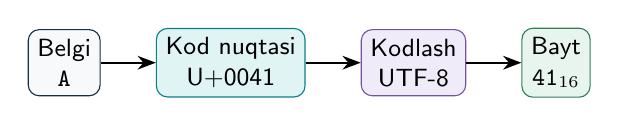
\begin{tikzpicture}[node distance=7mm,every node/.style={font=\sffamily\small,align=center}]
\node[draw=navy,fill=paper,rounded corners] (a) {Belgi\\\texttt{A}};
\node[draw=teal,fill=paleteal,rounded corners,right=of a] (b) {Kod nuqtasi\\U+0041};
\node[draw=purple,fill=palepurple,rounded corners,right=of b] (c) {Kodlash\\UTF-8};
\node[draw=greenx,fill=palegreen,rounded corners,right=of c] (d) {Bayt\\\texttt{41}$_{16}$};
\draw[-{Stealth},thick] (a)--(b);\draw[-{Stealth},thick] (b)--(c);\draw[-{Stealth},thick] (c)--(d);
\end{tikzpicture}
\end{center}

\term{Belgi} abstrakt mazmun birligi, \term{glif} uning ekrandagi shakli, \term{kod nuqtasi} Unicode ichidagi raqam, \term{kodlash} esa kod nuqtasini baytlarga aylantirish qoidasi. Bir belgi turli shriftlarda turli glifga ega bo'lishi mumkin.

\subsection{ASCII}
\term{ASCII} \eng{American Standard Code for Information Interchange}ning asl 7 bitli shakli 128 kodni ($0$--$127$) ifodalaydi. Darsliklarda ko'pincha 0--255 oralig'idagi 8 bitli ``ASCII'' deyiladi; texnik jihatdan bu turli \term{kengaytirilgan ASCII} kod sahifalaridir.

\begin{tabular}{>{\ttfamily}c>{\ttfamily}c>{\ttfamily}c l}
\toprule
Belgi & O'nlik & Ikkilik & Izoh\\
\midrule
@ & 64 & 01000000 & maxsus belgi\\
A & 65 & 01000001 & bosh harf\\
a & 97 & 01100001 & kichik harf\\
0 & 48 & 00110000 & raqam belgisi, son qiymati emas\\
\bottomrule
\end{tabular}

\begin{warningbox}
ASCII'dagi \texttt{'0'} belgisi kodi 48; bu sonning ikkilik qiymati 0 degani emas. Belgining kodi va sonning matematik qiymatini ajrating.
\end{warningbox}

\subsection{Unicode va UTF oilasi}
\term{Unicode} dunyo yozuv tizimlaridagi belgilar uchun yagona kod nuqtalari makonini belgilaydi. U+0041 -- A; kod nuqtasi o'zi diskdagi baytlar sonini aytmaydi.

\begin{tabularx}{\textwidth}{>{\bfseries\color{teal}}p{27mm}p{34mm}X}
\toprule
Kodlash & Birlik & Xususiyat\\
\midrule
UTF-8 & 1--4 bayt & ASCII bilan mos; lotin matnida ixcham; vebda keng tarqalgan.\\
UTF-16 & 2 yoki 4 bayt & Asosiy ko'p tilli tekislikdagi belgilar ko'pincha 2 bayt; surrogate juftlari mavjud.\\
UTF-32 & 4 bayt & Kod nuqtasiga bevosita kirish sodda, lekin hajm katta.\\
\bottomrule
\end{tabularx}

\subsubsection{Belgi soni har doim kod nuqtasi soniga teng emas}
Ko'rinadigan bitta grafema bazaviy harf va birlashtiruvchi diakritikdan tuzilishi mumkin. Emoji ham bir nechta kod nuqtasi ketma-ketligidan iborat bo'lishi mumkin. Shuning uchun ``ekrandagi belgilar'', ``Unicode kod nuqtalari'' va ``baytlar'' soni turlicha bo'lishi mumkin.

\subsection{Matn hajmi}
Doimiy $i$ bitli o'quv modelida:
\formula{V_{bit}=K\cdot i,\qquad V_B=\frac{K\cdot i}{8}}
$K$ -- barcha belgilar soni. Probel, satr oxiri, tabulyatsiya va tinish belgisi ham faylda kodlanadi.

\begin{examplebox}
2400 belgi 16 bitdan kodlansa: $2400\cdot16=38\,400$ bit $=4800$ B. Agar 1 KiB = 1024 B bo'lsa, $4800/1024\approx4.6875$ KiB.
\end{examplebox}

\subsection{Nega haqiqiy matn fayli formuladan farq qiladi?}
\begin{itemize}
\item UTF-8 o'zgaruvchan uzunlikda;
\item BOM yoki kodlash belgisi qo'shilishi mumkin;
\item satr oxiri LF yoki CRLF bo'lishi mumkin;
\item formatlangan hujjatda uslub, rasm va metadata mavjud;
\item siqish hajmni kamaytirishi mumkin.
\end{itemize}

\begin{attest}
Masalada ``har bir belgi 2 bayt'' deyilsa, Unicode'ning real o'zgaruvchanligini emas, berilgan doimiy modelni ishlating. Real standart savolida esa UTF turini aniqlash zarur.
\end{attest}

\subsection{Mustahkamlash: oddiydan murakkabga 3 misol}
\begin{taskbox}
\begin{enumerate}[leftmargin=7mm]
\item \textbf{Oddiy.} 120 belgili matnning har belgisi 1 bayt bo'lsa, hajmni toping.
\item \textbf{O'rta.} 300 ta kod nuqtasi UTF-16 soddalashtirilgan modelida 2 baytdan saqlansa, faylning xom matn qismi qancha?
\item \textbf{Murakkab.} UTF-8 matnda 80 ta ASCII belgi (1 bayt), 20 ta kirill belgi (2 bayt) va 5 ta emoji (4 bayt) bor. Faqat belgilar baytini hisoblang.
\end{enumerate}
\end{taskbox}

\begin{solutionbox}
\begin{enumerate}[leftmargin=7mm]
\item \textbf{Oddiy yechim.} $120\cdot1=120$ B.
\item \textbf{O'rta yechim.} $300\cdot2=600$ B. BOM, metadata va satr oxiri berilmaganligi uchun hisobga olinmaydi.
\item \textbf{Murakkab yechim.} $80\cdot1+20\cdot2+5\cdot4=80+40+20=140$ B. 105 ta ko'rinadigan belgi 105 bayt bo'lishi shart emas.
\end{enumerate}
\end{solutionbox}
\begin{attest}Unicode - kod nuqtalari standarti; UTF-8/16/32 - ularni baytlarga yozish usullari.\end{attest}

\begin{summarybox}
Unicode -- belgilar repertuari va kod nuqtalari; UTF-8/16/32 -- ularni baytlarga kodlash usullari. Matn hajmini hisoblashdan oldin kod uzunligi va hisoblanadigan belgilarni aniqlang.
\end{summarybox}
\begin{sourcebox}
ICT7, PDF 26--29; CAM1011, PDF 19--20; ICT5 kodlash bo'limi; OLD, 8-bob.
\end{sourcebox}

\section{Grafik axborot: rastr, vektor, rang va hajm}
\begin{keywordbox}
\term{rastr}, \term{vektor}, \term{piksel}, \term{rezolyutsiya}, \term{PPI}, \term{DPI}, \term{rang chuqurligi}, \term{palitra}, \term{RGB}, \term{CMYK}, \term{HSV}, \term{HSL}, \term{alfa-kanal}, \term{bitmap}.
\end{keywordbox}

\subsection{Rastr va vektor}
\begin{tabularx}{\textwidth}{>{\bfseries\color{navy}}p{30mm}X X}
\toprule
Mezon & Rastr & Vektor\\
\midrule
Saqlash & Piksel to'ri va rang qiymatlari & Nuqta, chiziq, egri, shakl va formulalar\\
Kattalashtirish & Piksel ko'rinishi, sifat pasayishi & Odatda sifat saqlanadi\\
Mos vazifa & Fotosurat, tekstura & Logo, diagramma, chizma\\
Tahrir & Piksel/soha bo'yicha & Obyekt xossalari bo'yicha\\
Format & BMP, PNG, JPEG, GIF, TIFF & SVG, EPS, AI; PDF aralash bo'lishi mumkin\\
\bottomrule
\end{tabularx}

\subsection{Piksel o'lchami va zichlik}
$W\times H$ -- tasvirning piksel o'lchami. \term{PPI} -- ekranda yoki tasvirda bir dyuymga piksel, \term{DPI} -- printer nuqtalari zichligi. 10 cm kenglikdagi tasvir 300 PPI bilan chop etilsa:
\formula{W_{px}=\frac{10}{2.54}\times300\approx1181\ px}

\begin{warningbox}
``1920×1080 rezolyutsiya'' piksel o'lchami; ``300 PPI'' zichlik. Ular bir xil kattalik emas.
\end{warningbox}

\subsection{Rang chuqurligi va palitra}
$i$ bit rang chuqurligi $2^i$ rang holatini beradi. 1 bit -- 2 rang, 8 bit -- 256, 24 bit -- taxminan 16.7 million. 32 bit ko'pincha 24 bit rang + 8 bit alfa shaffoflik.

\term{Indekslangan rang}da piksel to'g'ridan-to'g'ri RGB emas, palitra indeksini saqlaydi. Palitra faylda alohida saqlanadi.

\subsection{Rang modellari}
\begin{tabularx}{\textwidth}{>{\bfseries\color{teal}}p{28mm}X p{45mm}}
\toprule
Model & Prinsip & Qo'llanish\\
\midrule
RGB & Yorug'likni qo'shish; qora -- 0, oq -- kanallar maksimumi & monitor, kamera, veb\\
CMYK & Bo'yoqning yorug'likni yutishi; subtractive & bosma\\
HSV/HSL & Rang tusi, to'yinganlik va qiymat/yorug'lik & rang tanlash va tahrir\\
Grayscale & Yorqinlik darajalari & qora-oq tasvir va hujjat\\
\bottomrule
\end{tabularx}

\subsection{Siqilmagan rastr hajmi}
\formula{V_{bit}=W\cdot H\cdot i,\qquad V_B=\frac{WHi}{8}}
Bu formulaga odatda sarlavha, palitra, metadata, qator padding va siqish kirmaydi.

\begin{examplebox}
$1920\times1080$, 24 bit: $1920\cdot1080\cdot24=49\,766\,400$ bit $=6\,220\,800$ B $\approx5.93$ MiB. 60 ta kadr bo'lsa, faqat rastr ma'lumoti $\approx356$ MiB.
\end{examplebox}

\subsection{Grafik formatlar}
\begin{longtable}{>{\bfseries\color{navy}}p{22mm}p{35mm}p{44mm}p{44mm}}
\toprule
Format & Turi/siqish & Kuchli tomoni & Cheklovi\\
\midrule
\endfirsthead\toprule Format & Turi/siqish & Kuchli tomoni & Cheklovi\\\midrule\endhead
BMP & rastr, ko'pincha siqilmagan/RLE & sodda, pikselga yaqin & hajm katta\\
JPEG & rastr, yo'qotishli & fotosuratda kichik hajm & matn/chetda artefakt, alfa yo'q\\
PNG & rastr, yo'qotishsiz & shaffoflik, skrinshot, grafika & fotosuratda JPEGdan katta\\
GIF & palitrali, yo'qotishsiz LZW, animatsiya & sodda animatsiya & 256 rang cheklovi\\
TIFF & moslashuvchan rastr konteyner & skan, nashriyot, yuqori sifat & fayl katta, variantlari ko'p\\
SVG & vektor XML & masshtablash, veb ikonka & fotosurat uchun mos emas\\
WebP, AVIF & zamonaviy rastr, yo'qotishli yoki yo'qotishsiz & yuqori siqish, alfa/animatsiya & eski dastur mosligi\\
\bottomrule
\end{longtable}

\begin{attest}
Format tanlovi ``qaysi biri eng yaxshi'' emas: fotosurat, shaffof logo, tahrirlash, chop etish va brauzer mosligiga qarab tanlanadi.
\end{attest}

\subsection{Mustahkamlash: oddiydan murakkabga 3 misol}
\begin{taskbox}
\begin{enumerate}[leftmargin=7mm]
\item \textbf{Oddiy.} 100$\times$80 piksel oq-qora (1 bit/piksel) tasvirning xom hajmini toping.
\item \textbf{O'rta.} 640$\times$480 piksel, 24 bit rang chuqurligidagi rastr tasvir hajmini KiBda toping.
\item \textbf{Murakkab.} 1920$\times$1080 piksel, 32 bit/piksel tasvir 4:1 nisbatda siqildi. Siqilgan hajmni MiBda toping.
\end{enumerate}
\end{taskbox}

\begin{solutionbox}
\begin{enumerate}[leftmargin=7mm]
\item \textbf{Oddiy yechim.} $100\cdot80\cdot1=8000$ bit = 1000 B.
\item \textbf{O'rta yechim.} $640\cdot480\cdot24=7\,372\,800$ bit = 921 600 B = 900 KiB.
\item \textbf{Murakkab yechim.} Xom: $1920\cdot1080\cdot32/8=8\,294\,400$ B. Siqilgan: $8\,294\,400/4=2\,073\,600$ B $\approx1.98$ MiB. Header berilmagan.
\end{enumerate}
\end{solutionbox}
\begin{attest}Rastr hajm formulasida natija avval bit bo'ladi; bayt uchun 8 ga bo'ling.\end{attest}

\begin{summarybox}
Grafik hajmning asosiy omillari: piksel soni, rang chuqurligi, kadr/qatlamlar va siqish. Rastr formula bilan, vektor esa obyektlar murakkabligi bilan o'sadi.
\end{summarybox}
\begin{sourcebox}
ICT7, PDF 29--47; CAM1011, PDF 19--21; CAM9 tasvirlar bo'limi; ICT5 grafik muharrir bo'limi; OLD, 9-bob.
\end{sourcebox}

\section{Audioaxborot: namunalash, bit chuqurligi va hajm}
\begin{keywordbox}
\term{analog tovush}, \term{namuna olish}, \term{sampling rate}, \term{kvantlash}, \term{bit chuqurligi}, \term{kanal}, \term{mono}, \term{stereo}, \term{PCM}, \term{bitrate}, \term{WAV}, \term{MP3}, \term{FLAC}.
\end{keywordbox}

\subsection{Analogdan raqamligacha}
\begin{enumerate}
\item Mikrofon tovush bosimini elektr signaliga aylantiradi.
\item \term{Namuna olish chastotasi} sekundiga nechta o'lchov olinishini belgilaydi.
\item \term{Kvantlash} har namuna amplitudasini mavjud raqamli darajalardan biriga yaqinlashtiradi.
\item \term{Bit chuqurligi} bir namuna uchun darajalar sonini belgilaydi: $2^b$.
\item Namuna kodlari fayl yoki oqimga yoziladi; kerak bo'lsa siqiladi.
\end{enumerate}

\subsection{Namuna chastotasi va bit chuqurligi}
Namuna chastotasi Hz/kHzda. CD sifati odatda 44.1 kHz va 16 bit; telefon nutqi uchun ancha past chastota yetishi mumkin. Yuqori chastota yuqori tovush chastotalarini, yuqori bit chuqurligi esa amplituda nozikligini yaxshiroq ifodalaydi.

\begin{clarify}
Nyquist tamoyiliga ko'ra, eng yuqori $f$ chastotani qayta tiklash uchun ideal sharoitda namuna chastotasi $2f$ dan katta bo'lishi kerak. Amaliy tizimlarda filtr va zaxira diapazoni ham kerak.
\end{clarify}

\subsection{Siqilmagan PCM hajmi}
\formula{R=f_s\cdot b\cdot c}
\formula{V_{bit}=f_s\cdot b\cdot c\cdot t}
$f_s$ -- sample rate, $b$ -- bit depth, $c$ -- kanal, $t$ -- soniya.

\begin{examplebox}
44 100 Hz, 16 bit, stereo, 210 s:
$R=44\,100\cdot16\cdot2=1\,411\,200$ bit/s.
$V=1\,411\,200\cdot210/8=37\,044\,000$ B $\approx35.33$ MiB.
\end{examplebox}

\subsection{Siqilgan audio}
Tayyor bitrate berilsa:
\formula{V_{bit}=R\cdot t}
128 kb/s MP3 4 daqiqa: $128\,000\cdot240=30\,720\,000$ bit $=3.84$ MB (SI). VBRda bitrate vaqt bo'yicha o'zgaradi; o'rtacha bitrate ishlatiladi.

\subsection{Audio format va kodeklar}
\begin{tabularx}{\textwidth}{>{\bfseries\color{teal}}p{25mm}p{35mm}X}
\toprule
Format & Siqish & Xususiyat\\
\midrule
WAV & ko'pincha PCM, siqilmagan & tahrir uchun qulay, hajm katta; konteyner sifatida boshqa kodek ham bo'lishi mumkin\\
AIFF & ko'pincha PCM & Apple ekotizimida siqilmagan audio\\
MP3 & yo'qotishli & keng moslik, musiqa tarqatish\\
AAC & yo'qotishli & ko'pincha MP3ga nisbatan samaraliroq\\
FLAC & yo'qotishsiz & asl PCMni to'liq tiklaydi, hajmni kamaytiradi\\
OGG & konteyner/ekotizim & Vorbis yoki Opus kabi kodeklar bilan\\
MIDI & audio namuna emas & nota, asbob va boshqaruv hodisalari; ijroga bog'liq\\
\bottomrule
\end{tabularx}

\begin{warningbox}
MIDI mikrofon yozuvi emas. U ``qaysi nota, qachon, qaysi asbob'' kabi buyruqlarni saqlaydi; shuning uchun hajmi kichik, lekin inson ovozini bevosita saqlamaydi.
\end{warningbox}

\subsection{Mustahkamlash: oddiydan murakkabga 3 misol}
\begin{taskbox}
\begin{enumerate}[leftmargin=7mm]
\item \textbf{Oddiy.} 8 kHz, 8 bit, mono, 10 sekundlik PCM audio hajmini toping.
\item \textbf{O'rta.} 44.1 kHz, 16 bit, stereo, 30 sekundlik audio hajmini MiBda toping.
\item \textbf{Murakkab.} 128 kbit/s tayyor audio oqimining 4 daqiqalik hajmini MBda toping. Nega sample-rate formulasini ishlatmaymiz?
\end{enumerate}
\end{taskbox}

\begin{solutionbox}
\begin{enumerate}[leftmargin=7mm]
\item \textbf{Oddiy yechim.} $8000\cdot8\cdot1\cdot10=640\,000$ bit = 80 000 B.
\item \textbf{O'rta yechim.} $44\,100\cdot16\cdot2\cdot30=42\,336\,000$ bit = 5 292 000 B $\approx5.05$ MiB.
\item \textbf{Murakkab yechim.} $128\,000\cdot240/8=3\,840\,000$ B = 3.84 MB (SI). Bitrate tayyor kodlangan oqimni bevosita beradi; sample-rate va bit-depthni yana ko'paytirish ikki marta hisoblash bo'ladi.
\end{enumerate}
\end{solutionbox}
\begin{attest}Mono/stereo kanal sonini, sekund/minutni va bit/baytni albatta tekshiring.\end{attest}

\begin{summarybox}
Audio hajmi sample rate, bit depth, kanal va davomiylikka bog'liq. Tayyor bitrate berilgan bo'lsa, PCM parametrlarini yana ko'paytirmang.
\end{summarybox}
\begin{sourcebox}
ICT7, PDF 34--39; ICT6, PDF 115--126; CAM1011, PDF 20--21 va audio/video bo'limi; OLD, 10-bob.
\end{sourcebox}

\section{Video va multimedia: kadr, FPS, bitrate va hajm}
\begin{keywordbox}
\term{kadr}, \term{kadr chastotasi}, \term{rezolyutsiya}, \term{progressive}, \term{interlaced}, \term{bitrate}, \term{kodek}, \term{konteyner}, \term{streaming}, \term{buffering}, \term{animatsiya}, \term{multimedia}.
\end{keywordbox}

\subsection{Kadr va kadr chastotasi}
\term{Kadr} -- videodagi bitta tasvir. \term{Kadr chastotasi} \eng{fps} sekunddagi kadrlar soni. Ko'proq fps harakatni silliqlashtiradi, lekin xom hajm va kodlash yukini oshiradi.

\subsection{Siqilmagan video hajmi}
Audio qo'shilmagan xom video:
\formula{V_{bit}=W\cdot H\cdot d\cdot fps\cdot t}
$d$ -- pikselga bit. Audio alohida hisoblanib qo'shiladi.

\begin{examplebox}
$1280\times720$, 24 bit, 30 fps, 10 s:
$1280\cdot720\cdot24\cdot30\cdot10=6\,635\,520\,000$ bit $\approx829.44$ MB. Bu siqilmagan hajm; real H.264 fayli ancha kichik.
\end{examplebox}

\subsection{Bitrate asosidagi hajm}
\formula{V=(R_v+R_a)\cdot t}
Video 4 Mb/s, audio 128 kb/s, 5 daqiqa: $(4\,000+128)\text{ kb/s}\times300=1\,238\,400$ kb $=154.8$ MB (SI).

\subsection{Kodek va konteyner}
\begin{definition}
\term{Kodek} -- media oqimini kodlaydigan va dekodlaydigan algoritm/dastur. \term{Konteyner} -- video, audio, subtitr va metadata oqimlarini bitta fayl tuzilishida saqlovchi format.
\end{definition}

\begin{tabularx}{\textwidth}{>{\bfseries\color{navy}}p{32mm}X}
\toprule
Konteyner & Odatda uchraydigan xususiyat\\
\midrule
MP4 & H.264/H.265/AV1 video, AAC audio; keng moslik\\
MKV & ko'p audio/subtitr oqimi, moslashuvchan\\
AVI & eski Windows konteyneri; kodek turli bo'lishi mumkin\\
MOV & Apple QuickTime ekotizimi\\
WebM & veb uchun VP9/AV1 va Opus/Vorbis\\
\bottomrule
\end{tabularx}

Bir xil \texttt{.mp4} fayl ichida turli kodek bo'lishi mumkin; kengaytma dekoder mavjudligini kafolatlamaydi.

\subsection{Video siqish g'oyasi}
\begin{itemize}
\item \textbf{Intra-frame:} bitta kadr ichidagi ortiqcha ma'lumotni kamaytirish.
\item \textbf{Inter-frame:} ketma-ket kadrlar orasidagi o'zgarishni saqlash.
\item \textbf{Keyframe/I-frame:} to'liq tayanch kadr; boshqa kadrlar farq yoki harakat vektori bilan bog'lanadi.
\item \textbf{Chroma subsampling:} inson ko'zi rang tafsilotiga yorqinlikdan kamroq sezgirligidan foydalanish.
\end{itemize}

\subsection{Streaming va buffering}
\term{Streaming} fayl to'liq yuklanmasdan media oqimini ketma-ket uzatib ijro etish. \term{Buffer} tarmoq tebranishini yumshatish uchun oldindan yig'ilgan ma'lumot. Tarmoqning barqaror amaliy tezligi bitrate va overheadni qoplay olmasa, buffering uzilishi yuz beradi.

\subsection{Animatsiya va multimedia}
\begin{tabularx}{\textwidth}{>{\bfseries\color{teal}}p{27mm}X}
\toprule
Tushuncha & Farqlovchi belgi\\
\midrule
Video & Kamera orqali yozilgan yoki render qilingan uzluksiz kadrlar oqimi\\
Animatsiya & Kadr/obyekt xossalarini sun'iy o'zgartirib harakat taassuroti\\
GIF animatsiya & Cheklangan rangli rastr kadrlar; audio yo'q\\
Vektor animatsiya & Obyekt va transformatsiyalar; masshtablash qulay\\
Multimedia & Matn, grafika, audio, video, animatsiya va interaktivlik birligi\\
\bottomrule
\end{tabularx}

\subsection{Mustahkamlash: oddiydan murakkabga 3 misol}
\begin{taskbox}
\begin{enumerate}[leftmargin=7mm]
\item \textbf{Oddiy.} 320$\times$240 piksel, 24 bit rang chuqurligidagi bitta xom kadr hajmini toping.
\item \textbf{O'rta.} Yuqoridagi formatda 25 fps tezlikdagi 8 sekundlik xom video hajmini MBda toping.
\item \textbf{Murakkab.} Video 5 Mbit/s, audio 192 kbit/s. 12 daqiqalik multimedia oqimi hajmini MBda toping.
\end{enumerate}
\end{taskbox}

\begin{solutionbox}
\begin{enumerate}[leftmargin=7mm]
\item \textbf{Oddiy yechim.} $320\cdot240\cdot24=1\,843\,200$ bit = 230 400 B.
\item \textbf{O'rta yechim.} $230\,400\cdot25\cdot8=46\,080\,000$ B = 46.08 MB (SI).
\item \textbf{Murakkab yechim.} Umumiy bitrate $5000+192=5192$ kbit/s. Vaqt 720 s. Hajm $5192\cdot720/8=467\,280$ kB = 467.28 MB (SI). Konteyner overheadi berilmagan.
\end{enumerate}
\end{solutionbox}
\begin{attest}Xom video uchun piksel formulasi, tayyor oqim uchun bitrate formulasi ishlatiladi; ikkalasini bir masalada takror qo'llamang.\end{attest}

\begin{summarybox}
Video hajmini xom formula yoki tayyor bitrate modeli bilan hisoblang; ikkisini aralashtirmang. Konteyner oqimlarni saqlaydi, kodek ularni siqadi.
\end{summarybox}
\begin{sourcebox}
ICT7, PDF 34--39 va animatsiya bo'limlari; ICT6, audio-video formatlari; CAM1011, audio/video tahrirlash; CAM8 video va animatsiya; OLD, 11-bob.
\end{sourcebox}

\section{Format va kengaytma}
\subsection{Format va kengaytma}
\begin{definition}
\term{Fayl formati} -- ma'lumotning fayl ichida qanday tashkil etilishi va talqin qilinishini belgilovchi qoida. \term{Kengaytma} -- fayl nomining formatni ko'rsatishga xizmat qiladigan oxirgi qismi.
\end{definition}
Kengaytmani \texttt{.jpg}ga o'zgartirish Word hujjatini rasmga aylantirmaydi. Dastur format imzosi, header va \term{MIME type} orqali ichki turini aniqlashi mumkin.
\section{Raqamli tasvirlashning umumiy modeli}
Kompyuter matn, rasm, tovush yoki videoning “ma'nosi”ni bevosita saqlamaydi. U bitlar ketma-ketligini saqlaydi; fayl formati va dastur bu bitlarni qanday talqin qilishni belgilaydi.

\begin{center}
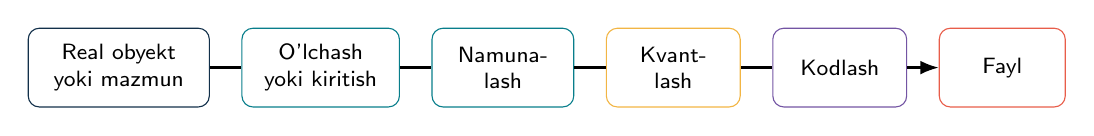
\begin{tikzpicture}[node distance=8mm and 4mm,every node/.style={font=\sffamily\footnotesize,align=center}]
\node[draw=Deep,rounded corners,minimum width=23mm,minimum height=10mm] (o) {Real obyekt\\yoki mazmun};
\node[draw=Blue,rounded corners,minimum width=20mm,minimum height=10mm,right=of o] (m) {O'lchash\\yoki kiritish};
\node[draw=Teal,rounded corners,minimum width=18mm,minimum height=10mm,right=of m] (s) {Namuna-\\lash};
\node[draw=Gold,rounded corners,minimum width=17mm,minimum height=10mm,right=of s] (q) {Kvant-\\lash};
\node[draw=Plum,rounded corners,minimum width=17mm,minimum height=10mm,right=of q] (e) {Kodlash};
\node[draw=Brick,rounded corners,minimum width=16mm,minimum height=10mm,right=of e] (f) {Fayl};
\draw[-{Latex},thick] (o)--(m)--(s)--(q)--(e)--(f);
\end{tikzpicture}
\end{center}

\term{Namunalash} uzluksiz jarayondan vaqt yoki makon bo'yicha nuqtalar olish; \term{kvantlash} har namuna qiymatini cheklangan darajalardan biriga yaqinlashtirish; \term{kodlash} natijani bitlar bilan ifodalashdir. Matnda namunalash bosqichi odatda yo'q, chunki matn avvaldan diskret belgilar ketma-ketligi. Tasvirda makon piksellarga, audioda vaqt namunalarga, videoda esa vaqt kadrlarga ajratiladi.

\begin{warningbox}{Hisoblangan xom hajm va haqiqiy fayl hajmi}
Formulalar odatda siqilmagan foydali ma'lumot hajmini beradi. Haqiqiy faylga sarlavha, metadata, rang profili, indeks, subtitr, xizmat bloklari va fayl tizimi xarajati qo'shilishi mumkin. Siqish esa hajmni kamaytiradi. Shuning uchun “formula natijasi” va “diskdagi fayl hajmi” doim aynan teng emas.
\end{warningbox}
\section{Audio va videoni chuqurroq tushuntiruvchi texnik tushunchalar}
\subsubsection{ADC va DAC}
Mikrofon tovush bosimini analog elektr signaliga aylantiradi. \term{ADC} analog signalni namunalab va kvantlab raqamli qiymatlarga o'tkazadi. Ijroda \term{DAC} raqamli namunalarni analog signalga, karnay esa uni tovush to'lqiniga aylantiradi.
\subsubsection{Namunalash chastotasi va Nyquist g'oyasi}
Namunalash chastotasi sekunddagi namuna soni. Nazariy jihatdan chastotasi $f_{max}$ gacha bo'lgan signalni tiklash uchun namunalash chastotasi kamida $2f_{max}$ dan katta bo'lishi kerak. Bu Nyquist-Shannon g'oyasidir. Amalda filtr va zaxira sabab biroz yuqori qiymat tanlanadi.
\subsubsection{Bit chuqurligi va kvantlash xatosi}
$d$ bit har namunaga $2^d$ daraja beradi. Bit chuqurligi oshsa amplituda aniqroq ifodalanadi va kvantlash shovqini kamayadi, ammo xom fayl hajmi ortadi. Namunalash chastotasi vaqt bo'yicha aniqlikni, bit chuqurligi amplituda aniqligini boshqaradi.
\subsubsection{PCM bit rate}
Siqilmagan PCM audio uchun:
\[
r=f_s\cdot d\cdot c,
\qquad V=r\cdot t.
\]
Masalan, 44,1 kHz, 16 bit, stereo oqimning xom tezligi $44\,100\cdot16\cdot2=1\,411\,200$ bit/s, ya'ni 1411,2 kbit/s.
\subsubsection{Kadrlararo siqish}
Video kodek har kadrni to'liq saqlash o'rniga ayrim tayanch kadrlar va kadrlar orasidagi o'zgarishni yozishi mumkin. Shu sababli siqilgan video hajmini $W\times H\times d\times FPS\times t$ bilan aniq topib bo'lmaydi; bitrate berilgan bo'lsa $V=r\cdot t$ ishlatiladi.
\subsubsection{Video formatlari va standartlar}
\begin{tabularx}{\textwidth}{>{\sffamily\bfseries}p{0.18\textwidth}p{0.24\textwidth}X}
\toprule
Atama & Turi & Izoh\\
\midrule
AVI, MP4, MKV, MOV, WebM & konteyner & audio, video, subtitr va metadata oqimlarini birlashtiradi\\
MPEG-1/2/4 & standartlar oilasi & CD, DVD, televideniye va raqamli media tarixida qo'llangan\\
H.264/AVC & video kodek & keng moslik va samarali siqish\\
H.265/HEVC, AV1 & video kodek & yuqori siqish samaradorligi, ko'proq hisoblash\\
WMV & Microsoft media oilasi & kodek/format nomi sifatida uchraydi\\
\bottomrule
\end{tabularx}
\section{Metadata va siqish algoritmlarining asosiy g‘oyalari}
\subsection{Metadata}
\term{Metadata} -- boshqa ma'lumot haqidagi ma'lumot: muallif, yaratilgan vaqt, kamera modeli, GPS, o'lcham, kodek, davomiylik, huquq va teglar. Metadata qidirish va boshqarishni osonlashtiradi, ammo maxfiy ma'lumotni ham oshkor qilishi mumkin.
\subsection{Asosiy siqish g'oyalari}
\subsubsection{RLE}
Takrorlanuvchi ketma-ketlikni ``son + qiymat'' bilan ifodalaydi. \texttt{AAAAABBBCC} $\rightarrow$ \texttt{5A3B2C}. Bir xil rangli sohalarda foydali, tasodifiy ma'lumotda hajmni oshirishi mumkin.

\subsubsection{Huffman/prefiks kod}
Tez-tez uchraydigan belgiga qisqa, kam uchraydiganga uzun kod beradi; daraxt asosidagi prefiks kod bir qiymatli dekodlanadi.

\subsubsection{Lug'atli siqish}
Takroriy satrlarni lug'at indekslari bilan almashtiradi; ZIP oilasida LZ usullari uchraydi.

\subsubsection{Perseptual siqish}
Inson sezgisi kam sezadigan qismlarni olib tashlaydi: JPEG yuqori chastotali tasvir detali, audio kodek maskalanadigan tovush, video kodek vaqt va rang ortiqchaligidan foydalanadi.
\section{Konvertatsiya, transkodlash, arxiv va zaxira}
\subsection{Konvertatsiya va transkodlash}

\begin{definition}
\keyterm{Konvertatsiya} — faylni bir format yoki tuzilmadan boshqasiga
o‘tkazish.
\end{definition}

\begin{definition}
\keyterm{Transkodlash} — media oqimini dekodlab, boshqa kodek yoki
sozlama bilan qayta kodlash.
\end{definition}

Yo‘qotishli faylni qayta-qayta yo‘qotishli kodlash sifatni har bosqichda
pasaytirishi mumkin. Faqat konteynerni almashtirib, ichki oqimni qayta
kodlamaslik \keyterm{remux} deyiladi; bunda sifat o‘zgarmaydi.

\begin{trap}
Yo‘qotishli MP3ni WAVga aylantirish yo‘qolgan tovushni qaytarmaydi.
WAV fayl kattalashadi, ammo manba sifati oshmaydi. Xuddi shunday,
JPEGni PNGga o‘tkazish oldingi JPEG artefaktlarini yo‘qotmaydi.
\end{trap}
\subsection{Arxiv va zaxira nusxasi farqi}

\begin{itemize}
  \item \keyterm{Arxivlash} — fayllarni bir to‘plamga joylash va ko‘pincha
  siqish (ZIP, 7z, RAR).
  \item \keyterm{Zaxira nusxasi} — yo‘qolish yoki buzilishdan tiklash uchun
  boshqa joyda nusxa saqlash.
\end{itemize}

Bir diskdagi yagona ZIP arxiv zaxira strategiyasi emas: disk buzilsa,
asl ham, arxiv ham yo‘qoladi.

\quickcheck{
\begin{enumerate}
  \item PNG va JPEGdan qaysi biri odatda yo‘qotishsiz?
  \item 100 MB fayl 25 MB bo‘lsa, koeffitsiyent va tejash foizi?
  \item Fayl kengaytmasini o‘zgartirish nega konvertatsiya emas?
\end{enumerate}}

\answers{
1) PNG. 2) \(4:1\), 75\%. 3) Ichki bayt tuzilishi va kodlash
o‘zgarmaydi; faqat nom o‘zgaradi.}

\begin{summarybox}
Yo‘qotishsiz siqishda asl nusxa aynan tiklanadi, yo‘qotishlida esa
qabul qilinadigan sifat evaziga katta hajm tejaladi. Format, kengaytma,
konteyner va kodekni alohida tushunish moslik savollarini yechadi.
\end{summarybox}

\begin{sourcebox}
Asosiy qamrov: ICT6, PDF 115–127; ICT10, PDF 29–31;
CAM8, PDF 124–126; CAM9, PDF 145–152; CAM10–11, PDF 19–23.
\end{sourcebox}
\section{Siqish natijasini va multimedia mahsulotini baholash}
\subsubsection{Siqish koeffitsiyenti va foiz kamayish}
Atamalar turlicha berilishi mumkin:
\[
K=\frac{V_{oldin}}{V_{keyin}},\qquad
\text{kamayish foizi}=\frac{V_{oldin}-V_{keyin}}{V_{oldin}}\cdot100\%.
\]
“4 marta siqildi” odatda yangi hajm eski hajmning $1/4$ qismi degani; “25\% ga kamaydi” esa yangi hajm 75\% qolganini bildiradi.

\begin{examplebox}{1-misol. Metrikani farqlash \difficulty{Oddiy}}
80 MB fayl 20 MB bo'ldi. Koeffitsiyent va kamayish foizi?
\begin{solutionbox}
$K=80/20=4$. Kamayish $(80-20)/80\cdot100\%=75\%$.
\end{solutionbox}
\end{examplebox}

\begin{examplebox}{2-misol. Foizdan yangi hajm \difficulty{O'rta}}
2,4 GB video hajmi 35\% ga kamaytirildi. Yangi hajm?
\begin{solutionbox}
65\% qoladi: $2,4\cdot0,65=1,56$ GB.
\end{solutionbox}
\end{examplebox}

\begin{examplebox}{3-misol. Ikki bosqichli qayta kodlash \difficulty{Murakkab}}
600 MB xom media avval 5 marta siqildi, so'ng olingan fayl yana 20\% ga kamaytirildi. Yakuniy hajm va umumiy koeffitsiyent?
\begin{solutionbox}
Birinchi hajm $600/5=120$ MB. Keyin $120\cdot0,8=96$ MB. Umumiy koeffitsiyent $600/96=6,25$ marta.
\end{solutionbox}
\end{examplebox}
\subsection{Multimedia mahsulotini maqsadga moslashtirish}
Multimedia hujjatida matn, tasvir, audio, video, animatsiya va interaktivlik bir maqsadga xizmat qilishi kerak. Har bir element qo'shilishi “ko'proq effekt” uchun emas, mazmunni aniqroq tushuntirish uchun asoslanadi.
\begin{itemize}
\item fayl formatini dastur va platforma mosligiga qarab tanlash;
\item katta media faylini sifatni maqbul saqlagan holda optimallashtirish;
\item subtitr, transkript, alt matn va yetarli kontrast bilan kirish imkoniyatini oshirish;
\item mualliflik va shaxsiy ma'lumot huquqlarini tekshirish;
\item auditoriya qurilmasi va internet tezligini hisobga olish;
\item autoplay, baland tovush va tez miltillash kabi noqulayliklardan saqlanish.
\end{itemize}

\sourcecite{Qo'shimcha sintez: ICT 6-, 7-, 8- va 10-sinf; Cambridge+ 6--10/11-sinf media bo'limlari; \textit{Ma'ruza (Tayyor)}, grafika va birliklar qismi.}

\begin{recapbox}
\begin{itemize}
\item Unicode kod nuqtalari tizimi, UTF esa baytga kodlash usuli.
\item Rastr hajmi piksel soni va rang chuqurligiga bog‘liq; vektor masshtabga chidamli.
\item Audio hajmi namuna chastotasi, bit chuqurligi, kanal va vaqt ko‘paytmasi.
\item Xom video hajmi rezolyutsiya, rang chuqurligi, FPS va vaqt ko‘paytmasi; siqilgan video ko‘pincha bitrate bilan hisoblanadi.
\item Kodek oqimni siqadi, konteyner oqimlarni bir faylda saqlaydi.
\item Format tanlashda sifat, hajm, tahrir, shaffoflik, moslik va auditoriyani birga baholang.
\end{itemize}
\end{recapbox}
\sourcecite{ICT7 26--38; ICT6 115--127; ICT10 29--31; CAM8 124--126; CAM9 119--152; CAM1011 10--31.}



\appendix
\section{Bob bo'yicha mustahkamlash savollari}
\begin{enumerate}
\item ASCII va Unicode orasidagi asosiy farq nima?
\item Rastr va vektor tasvirni masshtablash nuqtayi nazaridan taqqoslang.
\item Rang chuqurligi ikki baravar oshsa, xom rastr hajmiga qanday ta'sir qiladi?
\item Audio sifatiga namunalash chastotasi va bit chuqurligi qanday ta'sir ko'rsatadi?
\item Kodek, konteyner, format va kengaytmani bitta video fayl misolida ajrating.
\end{enumerate}

\chapter{Axborot hajmini hisoblashning yagona strategiyasi}
\chapterintro{Formula yodlashdan ko'ra, masala qaysi modelga tegishli ekanini aniqlash muhim. Har masalada avval axborot turi, siqish holati va birlik modeli belgilanadi.}

\begin{keywordbox}
\term{formula tanlash}, \term{birlik modeli}, \term{xom hajm}, \term{siqilgan hajm}, \term{bitrate}, \term{davomiylik}, \term{sig'im}, \term{teskari masala}, \term{overhead}, \term{yaxlitlash}.
\end{keywordbox}

\section{Yetti bosqichli yechim}
\begin{enumerate}
\item \textbf{Nima saqlanmoqda?} Matn, rastr, audio, video, tayyor oqim, arxiv yoki aralash media.
\item \textbf{Xom yoki siqilganmi?} Pixel/sample formulasi xom ma'lumotga; bitrate siqilgan oqimga ham tegishli bo'lishi mumkin.
\item \textbf{Berilganlarni belgilang.} Har bir qiymat yoniga birlik yozing.
\item \textbf{Bitta modelni tanlang.} Bir xil omilni ikki marta hisoblamang.
\item \textbf{Bit/baytni moslang.} Tezlik ko'pincha bit/s, fayl hajmi bayt.
\item \textbf{Hisoblang, yakunda aylantiring.} Oraliq bosqichda erta yaxlitlamang.
\item \textbf{Mantiqiy tekshiring.} Yuqori sifat hajmni kamaytirib yubormadimi? Vaqt va tezlik teskari bog'landimi?
\end{enumerate}

\section{Formula xaritasi}
\begin{longtable}{>{\bfseries\color{navy}}p{31mm}p{67mm}p{50mm}}
\toprule
Model & Formula & Asosiy birlik\\
\midrule
\endfirsthead\toprule Model & Formula & Asosiy birlik\\\midrule\endhead
Alifbo & $N=2^i$, $i=\lceil\log_2N\rceil$ & bit/belgi\\
Matn & $V=K\cdot i$ & bit\\
Rastr & $V=W\cdot H\cdot d$ & bit\\
PCM audio & $V=f_s\cdot b\cdot c\cdot t$ & bit\\
Xom video & $V=W\cdot H\cdot d\cdot fps\cdot t$ & bit\\
Tayyor bitrate & $V=R\cdot t$ & bit\\
Aralash oqim & $V=(R_v+R_a+R_{boshqa})t$ & bit\\
Uzatish & $t=V/R$ & sekund\\
Siqish nisbati & $V_s=V_a/k$ & bir xil birlik\\
Foizga kamayish & $V_s=V_a(1-r)$ & $r$ ulush\\
Sig'im & $n=\lfloor S/F\rfloor$ & butun fayl\\
\bottomrule
\end{longtable}

\section{Matn masalasi}
\begin{examplebox}
Alifbo 64 belgi, matn 12 000 belgi. Doimiy eng qisqa kod: $i=\log_2 64=6$ bit. Hajm $12\,000\cdot6=72\,000$ bit $=9\,000$ B. Agar har belgi 1 bayt deb alohida berilganida 12 000 B bo'lardi; ikki modelni aralashtirmang.
\end{examplebox}

\section{Grafik masalasi}
\begin{examplebox}
800×600 piksel, 256 rang. $d=\log_2 256=8$ bit. Xom hajm $800\cdot600\cdot8=3\,840\,000$ bit $=480\,000$ B. 3:1 siqilsa $160\,000$ B. Header va palitra kiritilmagan.
\end{examplebox}

\section{Audio masalasi}
\begin{examplebox}
22.05 kHz, 8 bit, mono, 2 daqiqa: $22\,050\cdot8\cdot1\cdot120=21\,168\,000$ bit $=2\,646\,000$ B. Agar 128 kb/s tayyor MP3 deyilsa, sample rate va bit depth formulasini emas, $128\,000\cdot120/8$ni ishlating.
\end{examplebox}

\section{Video masalasi}
\begin{examplebox}
1920×1080, 24 bit, 25 fps, 8 sekund xom video:
$1920\cdot1080\cdot24\cdot25\cdot8=9\,953\,280\,000$ bit $\approx1.244$ GB. Agar H.264 bitrate 6 Mb/s berilsa, hajm $6\,000\,000\cdot8/8=6\,000\,000$ B = 6 MB; xom parametrlar kerak emas.
\end{examplebox}

\section{Bir nechta oqimli media}
Video 5 Mb/s, audio 192 kb/s, subtitr 8 kb/s, 20 daqiqa:
\formula{R=5000+192+8=5200\ \text{kb/s}}
$V=5200\cdot1200=6\,240\,000$ kb $=780$ MB (SI). Konteyner overhead berilmasa e'tiborga olinmaydi.

\section{Xotiraga joylashtirish}
\begin{examplebox}
32 GiB bo'sh joyga 750 MiB fayl: $32\cdot1024=32\,768$ MiB. $\lfloor32\,768/750\rfloor=43$ fayl; qoldiq $518$ MiB. Agar qurilma 32 GB SI bo'lsa natija boshqacha.
\end{examplebox}

\section{Teskari masalalar}
\begin{itemize}
\item rasm rang chuqurligi: $d=8V/(WH)$;
\item audio davomiyligi: $t=8V/(f_sbc)$;
\item kanal tezligi: $R=8V/t$;
\item siqish koeffitsiyenti: $k=V_a/V_s$;
\item alifbo quvvati: $N=2^i$;
\item belgilar soni: $K=8V/i$.
\end{itemize}

\section{Yaxlitlash va sig'ish}
``Kamida nechta bit?'' -- yuqoriga yaxlitlanadi. ``Nechta to'liq fayl sig'adi?'' -- pastga, butun qism. Uzatish vaqti foydalanuvchiga butun sekund kerak bo'lsa, talabga qarab yuqoriga yaxlitlanishi mumkin. Oraliq qiymatlarda aniqlik saqlanadi.

\section{Mantiqiy nazorat}
\begin{enumerate}
\item Bit chuqurligi oshsa xom hajm oshishi kerak.
\item Ikki kanal mono hajmdan ikki marta katta.
\item Tezlik ikki marta oshsa vaqt yarmiga tushadi.
\item 60\% kamayishdan so'ng 40\% qoladi.
\item Siqilgan hajm koeffitsiyent $k>1$ bo'lsa kichik bo'lishi kerak.
\item Fayllar soni kasr bo'lmaydi.
\end{enumerate}

\begin{warningbox}
Eng ko'p xato: MBni Mb/sga to'g'ridan-to'g'ri bo'lish; 8 koeffitsiyenti yo'qoladi. Ikkinchi xato: xom video formulasi bilan berilgan bitrate'ni yana ko'paytirish.
\end{warningbox}

\section{Mustahkamlash: oddiydan murakkabga 3 misol}
\begin{taskbox}
\begin{enumerate}[leftmargin=7mm]
\item \textbf{Oddiy.} 1024$\times$768 piksel, 8 bit/piksel rasmning xom hajmini KiBda toping.
\item \textbf{O'rta.} 44.1 kHz, 16 bit, stereo, 90 s audio 3:1 nisbatda siqildi. Siqilgan hajmni MiBda toping.
\item \textbf{Murakkab.} Video 4.5 Mbit/s va audio 128 kbit/s. 2 GiB bo'sh joyga necha to'liq 30 daqiqalik fayl sig'adi? SI bitrate va IEC sig'imni ehtiyotkorlik bilan hisoblang.
\end{enumerate}
\end{taskbox}

\begin{solutionbox}
\begin{enumerate}[leftmargin=7mm]
\item \textbf{Oddiy yechim.} $1024\cdot768\cdot8/8=786\,432$ B = 768 KiB.
\item \textbf{O'rta yechim.} Xom: $44\,100\cdot16\cdot2\cdot90/8=15\,876\,000$ B. Siqilgan: $5\,292\,000$ B $\approx5.05$ MiB.
\item \textbf{Murakkab yechim.} Umumiy bitrate 4.628 Mbit/s. 1800 s fayl: $4.628\cdot10^6\cdot1800/8=1\,041\,300\,000$ B. 2 GiB = $2\cdot2^{30}=2\,147\,483\,648$ B. $\lfloor2\,147\,483\,648/1\,041\,300\,000\rfloor=2$ fayl.
\end{enumerate}
\end{solutionbox}
\begin{attest}Masala avval modelni tanlashdan boshlanadi: xom parametrmi yoki tayyor bitrate, SI yoki IEC, siqish oldinmi yoki keyinmi.\end{attest}

\begin{summarybox}
Masala formuladan emas, modeldan boshlanadi. ``Xom parametrlar bormi yoki tayyor bitrate?'' va ``SI yoki IEC?'' savollari ko'p xatoni oldindan yo'q qiladi.
\end{summarybox}
\begin{sourcebox}
ICT5/7 axborot birliklari; CAM1011 matn/tasvir/audio/video formulalari; test bankidagi A--E hisoblash modeli; OLD, 13--14-boblar.
\end{sourcebox}
\chapter{Attestatsiyadagi nozik farqlar va diagnostika}
\chapterintro{Quyidagi farqlar savol variantlarida ataylab bir-biriga yaqinlashtiriladi. Har juftlikni bitta aniq jumla bilan ajrata olish zarur.}

\section{Qirqta ``bir jumlada farq''}
\begin{longtable}{>{\bfseries\color{teal}}p{45mm}p{105mm}}
\toprule
Juftlik & Aniq farq\\
\midrule
\endfirsthead\toprule Juftlik & Aniq farq\\\midrule\endhead
Ma'lumot / axborot & axborot -- kontekst va mazmun berilgan ma'lumot\\
Axborot / bilim & bilim -- tajriba va qoidaga bog'lanib harakat/xulosaga xizmat qilgan axborot\\
Xabar / signal & xabar -- mazmuniy ketma-ketlik; signal -- uni fizik tashuvchi holat\\
Axborot / tashuvchi & mazmun va uni saqlovchi moddiy muhit\\
Statik / dinamik & dinamik manba o'zgarsa avtomatik yangilanadi\\
Birlamchi / ikkilamchi & joriy maqsad uchun birinchi qo'l / boshqa maqsadda avval yig'ilgan\\
Analog / raqamli & uzluksiz fizik qiymat / diskret kod qiymatlari\\
Kodlash / shifrlash & formatga o'tkazish / kalitsiz o'qishni qiyinlashtirish\\
Shifrlash / hashlash & shifrlash qaytariladigan; hash odatda bir yo'nalishli\\
Siqish / arxivlash & hajmni kamaytirish / fayllarni paketlash va ehtimol siqish\\
Format / kengaytma & ichki tuzilish / fayl nomidagi odatiy belgi\\
Kodek / konteyner & oqimni kodlash / oqimlarni faylda saqlash\\
Bit / bayt & ikkilik belgi / 8 bitli guruh\\
kB / KiB & 1000 B / 1024 B\\
Belgi / bayt & semantik belgi / saqlash birligi; tenglik kodlashga bog'liq\\
ASCII / Unicode & kichik tarixiy kod repertuari / global kod nuqtalari standarti\\
Unicode / UTF-8 & kod nuqtalari tizimi / baytli kodlash usuli\\
Rastr / vektor & piksel to'ri / geometrik obyektlar\\
PPI / DPI & piksel zichligi / printer nuqta zichligi\\
Rang chuqurligi / rezolyutsiya & piksel rang bitlari / piksel soni yoki zichlik\\
Sample rate / bit depth & sekunddagi namuna / namuna amplitudasi bitlari\\
Bitrate / baud & sekunddagi bit / sekunddagi signal belgisi\\
Bandwidth / throughput & nazariy imkoniyat / real uzatish\\
Latency / bandwidth & kechikish / vaqt birligidagi hajm\\
Simplex / half-duplex & bir yo'nalish / ikki yo'nalish navbat bilan\\
Serial / parallel & bitlar ketma-ket / bir nechta yo'lda bir vaqtda\\
Validatsiya / verifikatsiya & qoidaga moslik / manbaga mos ko'chirish\\
Range / limit check & ikki chegara / bitta chegara\\
Check digit / checksum & kod raqami / blok nazorat qiymati\\
Identifikatsiya / autentifikatsiya & kim deb da'vo / dalil bilan isbot\\
Autentifikatsiya / avtorizatsiya & kimligini tekshirish / ruxsatini tekshirish\\
Virus / worm & host faylga birikish / tarmoqda mustaqil tarqalish\\
Plagiat / copyright infringement & manbasiz o'ziniki qilish / huquqni ruxsatsiz buzish\\
Open source / freeware & kod va litsenziya ochiqligi / narx bepul bo'lishi\\
VR / AR & sun'iy muhitga immersiya / real muhit ustiga raqamli qatlam\\
\bottomrule
\end{longtable}

\section{Formula tanlash daraxti}
\begin{center}
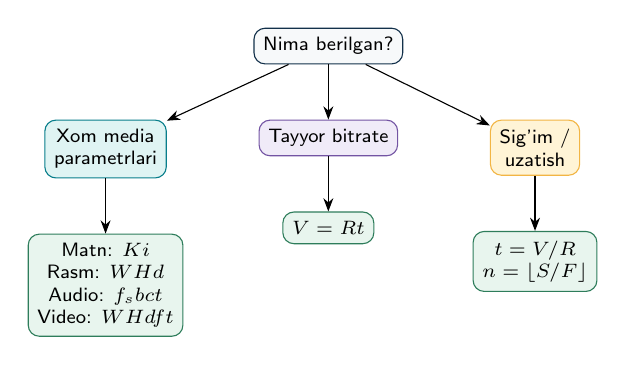
\begin{tikzpicture}[node distance=7mm and 11mm,every node/.style={font=\sffamily\scriptsize,align=center}]
\node[draw=navy,fill=paper,rounded corners] (q) {Nima berilgan?};
\node[draw=teal,fill=paleteal,rounded corners,below left=of q] (raw) {Xom media\\parametrlari};
\node[draw=purple,fill=palepurple,rounded corners,below=of q] (rate) {Tayyor bitrate};
\node[draw=gold,fill=palegold,rounded corners,below right=of q] (cap) {Sig'im /\\uzatish};
\node[draw=greenx,fill=palegreen,rounded corners,below=of raw] (type) {Matn: $Ki$\\Rasm: $WHd$\\Audio: $f_sbc t$\\Video: $WHdft$};
\node[draw=greenx,fill=palegreen,rounded corners,below=of rate] (rt) {$V=Rt$};
\node[draw=greenx,fill=palegreen,rounded corners,below=of cap] (ct) {$t=V/R$\\$n=\lfloor S/F\rfloor$};
\draw[-{Stealth}] (q)--(raw);\draw[-{Stealth}] (q)--(rate);\draw[-{Stealth}] (q)--(cap);
\draw[-{Stealth}] (raw)--(type);\draw[-{Stealth}] (rate)--(rt);\draw[-{Stealth}] (cap)--(ct);
\end{tikzpicture}
\end{center}

\section{Chalg'ituvchi gaplarni tuzatish}
\begin{enumerate}
\item ``Har bir belgi 1 bayt.'' $\rightarrow$ faqat berilgan kodlash 8 bit bo'lsa.
\item ``1 KB doimo 1024 B.'' $\rightarrow$ test modelida mumkin; standartda kB=1000 B, KiB=1024 B.
\item ``HTTPS sayt ishonchli mazmun beradi.'' $\rightarrow$ aloqa va identitet tekshiruviga yordam beradi, mazmun halolligini emas.
\item ``Validatsiya ma'lumot to'g'riligini kafolatlaydi.'' $\rightarrow$ faqat qoidaga moslikni tekshiradi.
\item ``Vektor faylning hajmi rezolyutsiyaga bog'liq.'' $\rightarrow$ asosan obyekt va murakkablikka; eksport qilingan rastrda rezolyutsiya muhim.
\item ``Asimmetrik shifrlash katta fayl uchun tezroq.'' $\rightarrow$ odatda sekin; katta trafik simmetrik shifr bilan.
\item ``Sinxronlash backupdir.'' $\rightarrow$ mustaqil, versiyali va tiklanadigan nusxa bo'lmasa, sinxronlashning o'zi backup emas.
\item ``Kod qisqa bo'lsa, ma'lumot xavfsiz.'' $\rightarrow$ kod jadvali ochilsa mazmun ochiladi.
\item ``Baud va bit/s bir xil.'' $\rightarrow$ faqat signal belgisi 1 bit tashisa.
\item ``Siqish va shifrlash bir xil.'' $\rightarrow$ siqish hajmni kamaytiradi, shifrlash esa kalitsiz o'qishni cheklaydi.
\end{enumerate}

\section{Diagnostika: 20 savol}
\begin{enumerate}
\item 50 ta holat uchun eng kam doimiy kod uzunligi nechta bit?
\item 1200 belgi 12 bitdan kodlansa hajmi necha bayt?
\item 1024×768, 16 bit rastrning xom hajmi necha bayt?
\item 8 kHz, 8 bit, mono, 30 s audio hajmi necha bayt?
\item 10 MB fayl 20 Mbit/sda ideal necha sekundda uzatiladi?
\item Statik va dinamik ma'lumotning farqini bir jumlada ayting.
\item Bevosita va bilvosita manbaga bittadan misol bering.
\item Kodlash, siqish va shifrlashni ASCII, ZIP, AES bilan moslang.
\item Sezar va Vijener shifrining kalitlari nimasi bilan farq qiladi?
\item Simmetrik va asimmetrik shifrlash qaysi vazifada birga ishlaydi?
\item UTF-8 bilan Unicode nimasi bilan farq qiladi?
\item PNG va JPEGni qaysi kontent uchun tanlaysiz?
\item Kodek va konteynerga bittadan misol bering.
\item Presence check nimani tekshirmaydi?
\item Ikki marta kiritish qaysi turdagi tekshiruv?
\item Hash maxfiylikni ta'minlaydimi?
\item Autentifikatsiya va avtorizatsiyani ajrating.
\item Phishingga qarshi eng muhim tekshiruv nima?
\item Backup va sinxronlash farqini ayting.
\item Raqamli imzo qaysi uch xususiyatga yordam beradi?
\end{enumerate}

\subsection*{Javoblar}
\begin{multicols}{2}
\begin{enumerate}
\item 6 bit ($2^5<50\le2^6$).
\item $1200\cdot12/8=1800$ B.
\item $1024\cdot768\cdot16/8=1\,572\,864$ B.
\item $8000\cdot8\cdot30/8=240\,000$ B.
\item $10\cdot8/20=4$ s (SI, overheadsiz).
\item Dinamik manba asosiy ma'lumot o'zgarsa avtomatik yangilanadi.
\item Yangi so'rov / eski statistik hisobot.
\item ASCII--kodlash; ZIP--siqish; AES--shifrlash.
\item Sezar -- bitta siljish; Vijener -- takrorlanuvchi kalit so'zning siljishlari.
\item TLS/HTTPS: asimmetrik ishonch/kalit, simmetrik trafik.
\item Unicode kod nuqtasi, UTF-8 baytli kodlash.
\item PNG -- logo/skrin/shaffof; JPEG -- foto.
\item H.264 kodek; MP4 konteyner.
\item Qiymatning to'g'ri yoki ma'noli ekanini emas, bo'sh emasligini.
\item Verifikatsiya.
\item Yo'q; yaxlitlik izini beradi, alohida shifrlash kerak.
\item Kimligini isbotlash / nima qilishga ruxsat.
\item Mustaqil rasmiy kanal orqali yuboruvchi va manzilni tekshirish.
\item Backup tiklash nusxasi; sync joriy holatni tenglashtiradi.
\item Autentiklik, yaxlitlik, inkor etmaslik.
\end{enumerate}
\end{multicols}

\section{Testni yakuniy tekshirish protokoli}
\begin{enumerate}
\item Savoldagi \textbf{asosiy fe'l}: ta'rifla, hisobla, farqla, tanla.
\item Birlik va prefiks: b/B, k/M/G, SI/IEC.
\item Model: xom/siqilgan, belgi/bayt, bitrate/baud.
\item Istisno: ``har doim'', ``faqat'', ``barcha'' kabi mutlaq so'z.
\item Atama jufti: validatsiya/verifikatsiya, kodlash/shifrlash.
\item Natija mantiqi: kattalik va yo'nalish.
\end{enumerate}

\section{Mustahkamlash: oddiydan murakkabga 3 misol}
\begin{taskbox}
\begin{enumerate}[leftmargin=7mm]
\item \textbf{Oddiy.} ``1 belgi = 1 bayt'' jumlasi qachon to'g'ri?
\item \textbf{O'rta.} ``Baud doimo bit/sga teng'' jumlasini qarshi misol bilan rad eting.
\item \textbf{Murakkab.} Bir savolda 800 MB rasm 25\% ga kamaydi va 10 Mbit/sda uzatildi. To'g'ri yakuniy vaqtni toping va ikkita ehtimoliy xatoni ayting.
\end{enumerate}
\end{taskbox}

\begin{solutionbox}
\begin{enumerate}[leftmargin=7mm]
\item \textbf{Oddiy yechim.} Faqat kodlash modeli har bir belgiga aynan 1 bayt ajratganda, masalan soddalashtirilgan 8 bitli kod jadvalida. UTF-8da umumiy qoida emas.
\item \textbf{O'rta yechim.} 16 holatli signal bir simvolda $\log_2 16=4$ bit tashiydi. 2400 baud $=9600$ bit/s; demak teng emas.
\item \textbf{Murakkab yechim.} Qolgan hajm $800\cdot0.75=600$ MB = 4800 Mbit. Vaqt $4800/10=480$ s = 8 min. Xatolar: 25\% qoladi deb olish; MBni Mbitga 8 ga ko'paytirmasdan bo'lish.
\end{enumerate}
\end{solutionbox}
\begin{attest}Nozik farqni bir jumla bilan ayta olish va birlikni yozish - attestatsiya xatolarini keskin kamaytiradi.\end{attest}

\begin{summarybox}
Attestatsiyada ko'p savol fakt yodlashdan ko'ra yaqin tushunchalar chegarasini tekshiradi. Javobni tanlashdan oldin savolning model, birlik va maqsadini bir jumlada qayta ifodalang.
\end{summarybox}
\begin{sourcebox}
Barcha asosiy darsliklar, professional test banki va OLD 19-bob asosida integratsion diagnostika.
\end{sourcebox}



\chapter{Bir qarashda: formulalar va birliklar}
\chapterintro{Bu ilova takrorlash uchun. Formulani ishlatishdan oldin
tegishli bobdagi shart va istisnoni bilish zarur.}

\section{Kod va axborot miqdori}

\begin{tabularx}{\textwidth}{@{}L{48mm}L{55mm}Y@{}}
\toprule
\textbf{Vazifa} & \textbf{Formula} & \textbf{Izoh}\\
\midrule
\(i\) bitdagi holatlar & \(N=2^i\) & teng uzunlikdagi ikkilik kod\\
\(N\) holat uchun bit & \(i=\lceil\log_2N\rceil\) & eng kichik butun bit\\
\(m\) belgili xabar & \(I=mi\) & \(i\) bit/belgi\\
\bottomrule
\end{tabularx}

\section{Birliklar}

\[
1~\B=8~\bit
\]
\[
1~\mathrm{KiB}=2^{10}\B,\quad
1~\mathrm{MiB}=2^{20}\B,\quad
1~\mathrm{GiB}=2^{30}\B,\quad
1~\mathrm{TiB}=2^{40}\B.
\]
\[
1~\mathrm{kB}=10^3\B,\quad
1~\mathrm{MB}=10^6\B,\quad
1~\mathrm{GB}=10^9\B,\quad
1~\mathrm{TB}=10^{12}\B.
\]

\section{Matn}

\[
I_{\bit}=(\text{sahifa})\cdot(\text{satr/sahifa})
\cdot(\text{belgi/satr})\cdot(\text{bit/belgi}).
\]

\section{Grafika}

\[
P=W\cdot H,\qquad N_{\text{rang}}=2^d,
\]
\[
I_{\bit}=W\cdot H\cdot d,\qquad
I_{\B}=\frac{W\cdot H\cdot d}{8}.
\]
\[
W_{\mathrm{px}}=\frac{W_{\mathrm{cm}}}{2.54}\cdot\mathrm{PPI},
\qquad
H_{\mathrm{px}}=\frac{H_{\mathrm{cm}}}{2.54}\cdot\mathrm{PPI}.
\]

\section{Audio}

\[
R_{\bit/\mathrm{s}}=f_s\cdot d\cdot c,
\]
\[
I_{\bit}=f_s\cdot d\cdot c\cdot t.
\]

\section{Video}

\[
I_{\bit}=W\cdot H\cdot d\cdot f\cdot t
\quad\text{(xom, audiosiz)}.
\]
\[
I_{\text{jami}}=I_{\text{video}}+I_{\text{audio}}.
\]

\section{Tayyor bit rate va uzatish}

\[
I=Rt,\qquad
v=\frac{I}{t},\qquad
t=\frac{I}{v}.
\]

\[
R_{\bit/\mathrm{s}}=R_{\mathrm{Bd}}\log_2M
\quad\text{(\(M\) holatli signal simvoli, ideal model)}.
\]

\section{Siqish va sig‘im}

\[
k=\frac{I_{\text{asl}}}{I_{\text{siqilgan}}},
\qquad
\text{tejash \%}=
\left(1-\frac{I_{\text{siqilgan}}}{I_{\text{asl}}}\right)100\%.
\]
\[
n_{\text{fayl}}=
\left\lfloor\frac{S_{\text{xotira}}}{I_{\text{fayl}}}\right\rfloor.
\]
\chapter*{Boblar bo'yicha A--E diagnostika}
\addcontentsline{toc}{chapter}{Boblar bo'yicha A--E diagnostika}
\section*{1-bob}
\begin{enumerate}
\item[A.] Informatika fanining eng to'liq predmetini bir jumlada yozing.
\item[B.] Ma'lumot va axborotni bitta misol bilan farqlang.
\item[C.] ``28'' qiymatini ma'lumotdan bilimga aylantiruvchi zanjir tuzing.
\item[D.] Xabar, signal va tashuvchining vazifalarini bitta aloqa vaziyatida ko'rsating.
\item[E.] Analog/raqamli va uzluksiz/diskret juftliklari nega aynan sinonim emasligini tushuntiring.
\end{enumerate}
\section*{2-bob}
\begin{enumerate}
\item[A.] Statik axborotga aniq ta'rif bering.
\item[B.] Birlamchi manba bilan bevosita manbani farqlang.
\item[C.] Ommaviy, ammo mualliflik huquqi bilan himoyalangan axborotga misol keltiring.
\item[D.] Rasmiy, lekin eskirgan ma'lumotning qaysi sifat xossalari kuchli va zaif bo'lishi mumkin?
\item[E.] Bir manbani birlamchi/ikkilamchi, bevosita/bilvosita va ichki/tashqi mezonlarida tahlil qiling.
\end{enumerate}
\section*{3-bob}
\begin{enumerate}
\item[A.] Filtrlash nima?
\item[B.] Saralash va guruhlashni farqlang.
\item[C.] ``axborot hajmi'' mavzusiga aniq qidiruv so'rovi tuzing.
\item[D.] Elektron xatda CC, BCC va Reply all tanlovini vaziyatga mos izohlang.
\item[E.] Manbasiz grafikni ulashishdan oldingi tekshiruv algoritmini yozing.
\end{enumerate}
\section*{4-bob}
\begin{enumerate}
\item[A.] 1 bayt necha bit?
\item[B.] 30 holat uchun eng kam kod uzunligini toping.
\item[C.] 12 KiB ni bitga o'tkazing.
\item[D.] 24 Mbit fayl 6 Mbit/s amaliy tezlikda qancha vaqtda uzatiladi?
\item[E.] Nazariy tezligi 100 Mbit/s, samaradorligi 72\% bo'lgan kanal orqali 540 MB fayl uzatish vaqtini toping.
\end{enumerate}
\section*{5-bob}
\begin{enumerate}
\item[A.] Rastr tasvirning eng kichik elementi nima?
\item[B.] Konteyner va kodekni farqlang.
\item[C.] 800$\times$600 piksel, 24 bit rang chuqurligidagi xom rasm hajmini toping.
\item[D.] 44.1 kHz, 16 bit, stereo, 30 sekundlik PCM audio hajmini toping.
\item[E.] 8 Mbit/s video va 192 kbit/s audio oqimli 12 minutlik multimedia fayl hajmini MBda hisoblang.
\end{enumerate}
\chapter*{Diagnostika javoblari}
\addcontentsline{toc}{chapter}{Diagnostika javoblari}
\small
\textbf{1-bob:} A) Axborot jarayonlari va ularni avtomatlashtirish usul-vositalarini o'rganuvchi fan. B--E) Tegishli ta'rif va farqlash mezonlari bo'yicha; E da raqamli ko'rinish diskret koddan foydalanadi, ammo ``analog/raqamli'' ifodalash usuli, ``uzluksiz/diskret'' esa qiymatlar tabiatini bildiradi.\\
\textbf{2-bob:} A) Manba avtomatik o'zgarmaguncha yoki qo'lda tahrir qilinmaguncha yangilanmaydigan axborot. B) Birlamchilik ma'lumotning vazifa uchun birinchi marta yig'ilishiga, bevositalik esa obyekt bilan to'g'ridan-to'g'ri aloqaga taalluqli. Qolgan javoblar mezonlar asosida baholanadi.\\
\textbf{3-bob:} A) Shartga mos yozuvlarni ko'rsatish. B) Saralash tartiblaydi, guruhlash toifalarga ajratadi. C) Masalan, \texttt{"axborot hajmi" formula filetype:pdf}. D--E) bobdagi protokollar asosida.\\
\textbf{4-bob:} A) 8 bit. B) $\lceil\log_2 30\rceil=5$ bit. C) $12\cdot1024\cdot8=98\,304$ bit. D) $24/6=4$ s. E) Amaliy tezlik $72$ Mbit/s; $540$ MB $=4320$ Mbit; vaqt $4320/72=60$ s.\\
\textbf{5-bob:} A) Piksel. B) Konteyner oqimlarni tashkil etadi, kodek oqimni kodlaydi/siqadi. C) $800\cdot600\cdot24=11\,520\,000$ bit $=1\,440\,000$ B $\approx1.44$ MB. D) $44\,100\cdot16\cdot2\cdot30=42\,336\,000$ bit $=5\,292\,000$ B $\approx5.292$ MB. E) Jami $8.192$ Mbit/s; $720$ s da $5898.24$ Mbit $=737.28$ MB.
\normalsize



\chapter{Atamalar lug‘ati}
\chapterintro{Ta’rifni yodlashdan ko‘ra, har bir atamani qarama-qarshi
yoki yaqin tushunchasi bilan birga takrorlang.}

\small
\begin{longtable}{@{}L{38mm}L{127mm}@{}}
\toprule
\textbf{Atama} & \textbf{Qisqa, testga mos ta’rif}\\
\midrule
\endhead
ADC & analog signalni raqamli namunalarga aylantiruvchi qurilma.\\
Alfa kanal & piksel shaffofligini ifodalovchi qo‘shimcha kanal.\\
Alifbo & kodlashda ruxsat etilgan belgilar to‘plami.\\
Alifbo quvvati & alifbodagi turli belgilar soni.\\
Analog signal & qiymati uzluksiz o‘zgarishi mumkin bo‘lgan signal.\\
Animatsiya & kadr/obyekt holatlarini ketma-ket ko‘rsatib harakat taassuroti yaratish.\\
ASCII & asosiy lotin va boshqaruv belgilarining 7 bitli standart kodi.\\
Asimmetrik shifrlash & ochiq va yopiq kalit juftiga asoslangan shifrlash.\\
AT & axborot jarayonlari uchun usul, dastur, texnika va insonlar majmui.\\
Audio bit tezligi & bir sekund audio oqimiga ishlov beriladigan bitlar soni.\\
Autentifikatsiya & foydalanuvchi da’vo qilgan shaxs ekanini tekshirish.\\
Avtorizatsiya & tasdiqlangan foydalanuvchiga ruxsatlarni belgilash.\\
Axborot & kontekst va mazmunga ega, qabul qiluvchi uchun ma’noli ma’lumot.\\
Axborot kanali & signal manbadan qabul qiluvchiga o‘tadigan muhit.\\
Axborot madaniyati & axborotni topish, baholash, qonuniy va xavfsiz ishlatish qobiliyati.\\
Axborot manbai & xabarni hosil qiluvchi yoki yuboruvchi subyekt/obyekt.\\
Axborot obyekti & axborotni ifodalovchi matn, rasm, model va boshqa obyekt.\\
Axborot tashuvchi & axborot saqlanadigan moddiy muhit.\\
Axborotli jarayon & axborotni yaratish yoki uning ustida bajariladigan amal.\\
Bandwidth & kanalning nazariy yoki belgilangan maksimal uzatish quvvati.\\
Baud & sekunddagi signal/modulyatsiya simvollari soni, Bd.\\
Bayt & 8 bitdan iborat birlik.\\
Bevosita manba & ayni foydalanish maqsadi uchun to‘plangan ma’lumot.\\
Bilim & axborotning tajriba va qoidalar bilan bog‘langan o‘zlashtirilgan shakli.\\
Bilimlar bazasi & xulosa uchun fakt va qoidalar tartibli majmui.\\
Bilvosita manba & avval boshqa maqsadda to‘plangan ma’lumot.\\
Bit & 0/1 ikkilik birligi; ikki teng holatdan birini ajratish miqdori.\\
Bit chuqurligi & namuna yoki pikselga ajratilgan bitlar soni.\\
Bit tezligi & sekundda uzatilgan yoki ishlov berilgan bitlar soni.\\
Braille & bo‘rtma nuqtalarga asoslangan taktil yozuv tizimi.\\
Brainware & axborot tizimidagi insonlar va ularning kompetensiyasi.\\
Checksum & blok qiymatlaridan hisoblangan xato nazorat yig‘indisi.\\
CIA triadasi & maxfiylik, yaxlitlik va mavjudlik uchligi.\\
CMYK & bosmada qo‘llanadigan ayriluvchi rang modeli.\\
Codec & media oqimini kodlaydigan/siqadigan va dekodlaydigan modul.\\
CRC & polinomli hisobga asoslangan xato aniqlash kodi.\\
DAC & raqamli namunani analog signalga aylantiruvchi qurilma.\\
Dekodlash & koddan dastlabki mazmunni tiklash.\\
Deshifrlash & shifrmatnni tegishli kalit bilan ochish.\\
Dezinformatsiya & ataylab aldash uchun tarqatilgan chalg‘ituvchi axborot.\\
Diskret signal & ajratilgan vaqt/qiymatlarda ifodalangan signal.\\
Dinamik ma’lumot & manba o‘zgarishi bilan avtomatik yangilanadigan ma’lumot.\\
DPI & bosmada bir dyuymga to‘g‘ri keladigan nuqtalar soni.\\
Fayl formati & fayl ichki ma’lumotining tuzilish va kodlanish qoidasi.\\
Fayl kengaytmasi & nom oxiridagi formatni ko‘rsatuvchi belgi.\\
Fayl hajmi & fayldagi axborot yoki xotirada egallagan joy miqdori.\\
Fayervol & trafikni qoidalar bo‘yicha ruxsatlaydigan yoki bloklaydigan vosita.\\
Filtrlash & mezonga mos bo‘lmagan yozuvlarni chiqarib tashlash.\\
Format tekshiruvi & qiymat belgilangan andazaga mosligini tekshirish.\\
FPS & sekundda ko‘rsatiladigan video kadrlari soni.\\
Fraktal grafika & matematik takrorlanuvchi qoida bilan hosil qilinadigan grafika.\\
Goodput & foydalanuvchining foydali yuk ma’lumoti tezligi.\\
Grafik axborot & rasm, chizma, sxema yoki diagramma shaklidagi axborot.\\
Hash & ma’lumotdan hisoblangan doimiy uzunlikdagi bir yo‘nalishli dayjest.\\
Identifikatsiya & foydalanuvchining kimligini da’vo qilishi.\\
IEC prefiksi & KiB, MiB kabi 2 darajalariga asoslangan prefiks.\\
Informatika & axborot jarayonlari va ularni avtomatlashtirishni o‘rganuvchi fan.\\
Internet & o‘zaro bog‘langan global tarmoqlar tizimi.\\
Ishonchlilik & axborot va manbaga asosli ishonish mumkinligi.\\
Kadr & videodagi bitta alohida tasvir.\\
Kanal & alohida audio oqimi yoki axborot uzatish muhiti; kontekstga qaraladi.\\
Kechikish & signal/paket yetib borishiga ketgan vaqt.\\
Kod & elementlar o‘rtasidagi belgili moslashtirish qoidalari.\\
Kod nuqtasi & Unicode repertuaridagi belgiga berilgan abstrakt son.\\
Kodlash & axborotni belgilangan kod yoki formatga o‘tkazish.\\
Konteyner & video, audio, subtitr kabi oqimlarni bitta faylda jamlovchi tuzilma.\\
Kriptoanaliz & shifr xavfsizligi va uni ochish usullarini tahlil qilish.\\
Kriptografiya & axborotni matematik usullar bilan himoyalash sohasi.\\
Latentlik & qarang: kechikish.\\
Litsenziya & asardan foydalanish ruxsatlari va shartlari.\\
Ma’lumot & hali kontekst va talqin berilmagan belgilar/kuzatuvlar.\\
Mavjudlik & ruxsatli foydalanuvchi axborotga vaqtida kira olishi.\\
Maxfiylik & axborotni faqat ruxsat etilgan subyekt ko‘rishi.\\
Metama’lumot & boshqa ma’lumotning muallifi, vaqti, formati kabi tavsifi.\\
MFA & turli omillardan kamida ikkitasiga asoslangan autentifikatsiya.\\
Misinformatsiya & noto‘g‘ri, lekin albatta qasddan bo‘lmagan axborot.\\
Morse kodi & qisqa va uzun signallar bilan belgilarni ifodalash tizimi.\\
Multimedia & matn, grafika, audio, video va interaktivlikning uyg‘unligi.\\
Mualliflik huquqi & ijodkorning asariga nisbatan qonuniy huquqlari.\\
Namuna chastotasi & bir sekundda olingan audio namunalar soni, Hz.\\
Nazorat raqami & identifikator xatosini tekshirish uchun hisoblangan belgi.\\
Obyektivlik & faktning shaxsiy manfaat va fikrdan imkon qadar ajratilishi.\\
Ommaviy mulk & mualliflik cheklovi amal qilmaydigan asarlar sohasi.\\
Paritet biti & 1 lar sonining juft/toqligini nazorat qiluvchi ortiqcha bit.\\
Phishing & sirni kiritishga aldovchi soxta xabar yoki sayt usuli.\\
Piksel & rastr/ekrandagi eng kichik alohida rang elementi.\\
Plagiat & boshqa muallif natijasini manbasiz o‘ziniki qilib ko‘rsatish.\\
Pozitsiyali sistema & raqam qiymati razryadiga bog‘liq sanoq sistemasi.\\
PPI & tasvirda bir dyuymga to‘g‘ri keladigan piksel soni.\\
Prefiks kod & hech bir kod so‘zi boshqasining bosh qismi bo‘lmagan kod.\\
Qabul qiluvchi & xabar yetib boradigan shaxs yoki tizim.\\
Qidiruv tizimi & veb-resurslarni indekslab, so‘rovga mos natija beruvchi xizmat.\\
Rang chuqurligi & bitta piksel rangiga ajratilgan bitlar soni.\\
Raqam & son yozuvida ishlatiladigan alohida belgi.\\
Raqamli axborot & diskret kodlarda ifodalangan axborot.\\
Raqamli imzo & kelib chiqish va yaxlitlikni tekshiruvchi kriptografik mexanizm.\\
Raqamli iz & raqamli faoliyat natijasida qolgan yozuvlar.\\
Rastr & piksel panjarasiga asoslangan grafik tasvir.\\
RGB & ekranda qizil, yashil, ko‘k yorug‘likni qo‘shuvchi model.\\
RLE & ketma-ket bir xil qiymatlarni takror soni bilan ifodalash siqishi.\\
Saralash & yozuvlarni tanlangan tartibga joylashtirish.\\
Sezar shifri & harflarni alifboda bir xil miqdorga siljitish shifri.\\
Signal & axborotni tashuvchi fizik holat yoki jarayon.\\
SI prefiksi & kB, MB kabi 10 darajalariga asoslangan prefiks.\\
Simplex & axborot faqat bir yo‘nalishda uzatiladigan rejim.\\
Simmetrik shifrlash & bir maxfiy kalit bilan shifrlash va ochish.\\
Siqish & axborotni kamroq bit bilan ifodalash.\\
Statik ma’lumot & o‘z-o‘zidan yangilanmaydigan ma’lumot.\\
Tahdid & zarar keltirishi mumkin bo‘lgan hodisa yoki subyekt.\\
Throughput & amalda vaqt birligida yetkazilgan jami ma’lumot.\\
To‘liqlik & vazifa uchun zarur qismlarning mavjudligi.\\
URL & Internet/WWW resursining manzili.\\
UTF-8 & Unicode kod nuqtalarini 1–4 bayt bilan ifodalovchi kodlash.\\
Validatsiya & ma’lumotning oldindan belgilangan qoidaga mosligini tekshirish.\\
Vektor & geometrik obyekt va formulalarga asoslangan grafika.\\
Verifikatsiya & kiritilgan ma’lumotning asl manbaga mosligini tekshirish.\\
WWW & Internet orqali taqdim etiladigan o‘zaro havolali veb-resurslar.\\
Xartli formulasi & \(N=2^i\) — \(i\) bitdagi teng uzunlikli holatlar soni.\\
Xavf & tahdidning zaiflikdan foydalanish ehtimoli va oqibati.\\
Xabar & axborotni yetkazish uchun tuzilgan belgilar/signallar ketma-ketligi.\\
Yaxlitlik & axborotning ruxsatsiz o‘zgarmasligi va to‘liqligi.\\
Yo‘qotishli siqish & ayrim asl ma’lumotni qaytarmasdan hajmni kamaytirish.\\
Yo‘qotishsiz siqish & original bitlarni to‘liq tiklaydigan siqish.\\
Zaiflik & tahdid foydalanishi mumkin bo‘lgan kamchilik.\\
Zaxira nusxasi & yo‘qolish yoki buzilishdan tiklash uchun qo‘shimcha nusxa.\\
\bottomrule
\end{longtable}
\normalsize

\chapter{Birlashtirish qamrovi va manba reyestri}
\section{Birlashtirish auditi}

\begin{sourcebox}{Birlashtirilgan fayllar}
\begin{enumerate}[leftmargin=8mm,itemsep=1mm]
\item \textbf{TEX 1:} \path{Axborotlar_3_0(1).tex}
\item \textbf{TEX 2:} \path{I_qism_Axborot_va_raqamli_savodxonlik_qayta_ishlangan(1).tex}
\item \textbf{TEX 3:} \path{Axborot_va_raqamli_savodxonlik(1).tex}
\item \textbf{ZIP loyiha:} \path{Axborot_va_axborot_jarayonlari_LaTeX.zip}
\end{enumerate}
\end{sourcebox}

\begin{longtable}{L{0.16\textwidth}L{0.38\textwidth}L{0.36\textwidth}}
\toprule
\textbf{Manba} & \textbf{Asosiy noyob hissasi} & \textbf{Yagona nashrdagi joyi}\\
\midrule
\endfirsthead
\toprule
\textbf{Manba} & \textbf{Asosiy noyob hissasi} & \textbf{Yagona nashrdagi joyi}\\
\midrule
\endhead
TEX 1 & Axborot texnologiyasi, raqamli jamiyat, accessibility, grafik halolligi, xato aniqlash, uzatish kanali, metadata, siqish algoritmlari, mualliflik va diagnostika. & 3-, 4-, 5-boblar va A--B ilovalar.\\
TEX 2 & Kengaytirilgan tasnif, dalil auditi, kod sig‘imi, tabiiy/formal til, Nyquist, ADC/DAC, kadrlararo siqish, multimedia moslashtirish. & Barcha besh bobdagi “chuqurlashtirish” bo‘limlari.\\
TEX 3 & Asosiy besh boblik didaktik oqim, sodda ta’riflar, bosqichli misollar, bob savollari va A--E diagnostika. & Har bobning asosiy matni va diagnostika ilovasi.\\
ZIP loyiha & Navy--Teal--Gold dizayn tizimi, muqova, tipografiya, kolontitul, bloklar; URL, transkodlash, arxiv/zaxira, formula varag‘i va keng lug‘at. & Butun nashr dizayni, 3- va 5-bob, formula hamda lug‘at ilovalari.\\
\bottomrule
\end{longtable}

\section{Mavzu chegarasi}
\begin{scopebox}
Ushbu nashrga faqat “I QISM. Axborot va raqamli savodxonlik asoslari”ning tasdiqlangan besh bobi kiritildi. Sanoq sistemalarining mustaqil kursi, sonlarning mashina xotirasida ifodalanishi, tarmoq topologiyalari va IP manzillash, ma’lumotlar bazasi, dasturiy ta’minot, algoritmlash va dasturlash tegishli keyingi qismlarga qoldirildi. Shifrlash, xavfsizlik va aloqa mavzularidan esa kodlash farqi, maxfiylik, kundalik xavfsizlik va axborot uzatish hajmini tushunish uchun zarur bo‘lgan kesishuvchi qismlar olindi.
\end{scopebox}

\section{Takrorlarni bartaraf etish qoidasi}
\begin{enumerate}
\item Bir xil ta’riflarning eng aniq va tushunarli varianti asosiy matnga olindi.
\item Qo‘shimcha ilmiy nozikliklar “chuqurlashtirish” yoki “aniqlashtirish” blokiga qo‘shildi.
\item Bir xil hisoblash usulidagi takroriy masalalardan metodik jihatdan kuchlisi qoldirildi; yangi shart yoki yangi xato turini ko‘rsatadigan masala saqlandi.
\item Bir-biriga zid soddalashtirishlarda test modeli va texnik standart alohida ko‘rsatildi.
\end{enumerate}

\begin{summarybox}
Yagona nashrning tuzilishi: besh asosiy bob, integratsion hisoblash strategiyasi, attestatsiya diagnostikasi, formulalar, A--E diagnostika, lug‘at va manba auditi. Dizayn ZIP loyihasidan, mazmun esa to‘rt manbaning takrorsiz sintezidan shakllantirildi.
\end{summarybox}

\printindex
\backmatter
\chapter*{Yakuniy eslatma}
\addcontentsline{toc}{chapter}{Yakuniy eslatma}
Bu fayl bitta mustaqil LaTeX manba sifatida tuzilgan: tashqi \texttt{chapters/*.tex} fayllariga bog‘liq emas. XeLaTeX va makeindex yordamida kompilyatsiya qilinadi.
\end{document}
